\documentclass[twoside]{book}

% Packages required by doxygen
\usepackage{fixltx2e}
\usepackage{calc}
\usepackage{doxygen}
\usepackage[export]{adjustbox} % also loads graphicx
\usepackage{graphicx}
\usepackage[utf8]{inputenc}
\usepackage{makeidx}
\usepackage{multicol}
\usepackage{multirow}
\PassOptionsToPackage{warn}{textcomp}
\usepackage{textcomp}
\usepackage[nointegrals]{wasysym}
\usepackage[table]{xcolor}

% Font selection
\usepackage[T1]{fontenc}
\usepackage[scaled=.90]{helvet}
\usepackage{courier}
\usepackage{amssymb}
\usepackage{sectsty}
\renewcommand{\familydefault}{\sfdefault}
\allsectionsfont{%
  \fontseries{bc}\selectfont%
  \color{darkgray}%
}
\renewcommand{\DoxyLabelFont}{%
  \fontseries{bc}\selectfont%
  \color{darkgray}%
}
\newcommand{\+}{\discretionary{\mbox{\scriptsize$\hookleftarrow$}}{}{}}

% Page & text layout
\usepackage{geometry}
\geometry{%
  a4paper,%
  top=2.5cm,%
  bottom=2.5cm,%
  left=2.5cm,%
  right=2.5cm%
}
\tolerance=750
\hfuzz=15pt
\hbadness=750
\setlength{\emergencystretch}{15pt}
\setlength{\parindent}{0cm}
\setlength{\parskip}{3ex plus 2ex minus 2ex}
\makeatletter
\renewcommand{\paragraph}{%
  \@startsection{paragraph}{4}{0ex}{-1.0ex}{1.0ex}{%
    \normalfont\normalsize\bfseries\SS@parafont%
  }%
}
\renewcommand{\subparagraph}{%
  \@startsection{subparagraph}{5}{0ex}{-1.0ex}{1.0ex}{%
    \normalfont\normalsize\bfseries\SS@subparafont%
  }%
}
\makeatother

% Headers & footers
\usepackage{fancyhdr}
\pagestyle{fancyplain}
\fancyhead[LE]{\fancyplain{}{\bfseries\thepage}}
\fancyhead[CE]{\fancyplain{}{}}
\fancyhead[RE]{\fancyplain{}{\bfseries\leftmark}}
\fancyhead[LO]{\fancyplain{}{\bfseries\rightmark}}
\fancyhead[CO]{\fancyplain{}{}}
\fancyhead[RO]{\fancyplain{}{\bfseries\thepage}}
\fancyfoot[LE]{\fancyplain{}{}}
\fancyfoot[CE]{\fancyplain{}{}}
\fancyfoot[RE]{\fancyplain{}{\bfseries\scriptsize Generated by Doxygen }}
\fancyfoot[LO]{\fancyplain{}{\bfseries\scriptsize Generated by Doxygen }}
\fancyfoot[CO]{\fancyplain{}{}}
\fancyfoot[RO]{\fancyplain{}{}}
\renewcommand{\footrulewidth}{0.4pt}
\renewcommand{\chaptermark}[1]{%
  \markboth{#1}{}%
}
\renewcommand{\sectionmark}[1]{%
  \markright{\thesection\ #1}%
}

% Indices & bibliography
\usepackage{natbib}
\usepackage[titles]{tocloft}
\setcounter{tocdepth}{3}
\setcounter{secnumdepth}{5}
\makeindex

% Hyperlinks (required, but should be loaded last)
\usepackage{ifpdf}
\ifpdf
  \usepackage[pdftex,pagebackref=true]{hyperref}
\else
  \usepackage[ps2pdf,pagebackref=true]{hyperref}
\fi
\hypersetup{%
  colorlinks=true,%
  linkcolor=blue,%
  citecolor=blue,%
  unicode%
}

% Custom commands
\newcommand{\clearemptydoublepage}{%
  \newpage{\pagestyle{empty}\cleardoublepage}%
}

\usepackage{caption}
\captionsetup{labelsep=space,justification=centering,font={bf},singlelinecheck=off,skip=4pt,position=top}

%===== C O N T E N T S =====

\begin{document}

% Titlepage & ToC
\hypersetup{pageanchor=false,
             bookmarksnumbered=true,
             pdfencoding=unicode
            }
\pagenumbering{alph}
\begin{titlepage}
\vspace*{7cm}
\begin{center}%
{\Large Machine Learning Toolkit \\[1ex]\large V0.\+1 }\\
\vspace*{1cm}
{\large Generated by Doxygen 1.8.13}\\
\end{center}
\end{titlepage}
\clearemptydoublepage
\pagenumbering{roman}
\tableofcontents
\clearemptydoublepage
\pagenumbering{arabic}
\hypersetup{pageanchor=true}

%--- Begin generated contents ---
\chapter{Hierarchical Index}
\section{Class Hierarchy}
This inheritance list is sorted roughly, but not completely, alphabetically\+:\begin{DoxyCompactList}
\item \contentsline{section}{Classifier}{\pageref{class_classifier}}{}
\begin{DoxyCompactList}
\item \contentsline{section}{Dual\+Classifier}{\pageref{class_dual_classifier}}{}
\begin{DoxyCompactList}
\item \contentsline{section}{Perceptron\+Dual}{\pageref{class_perceptron_dual}}{}
\item \contentsline{section}{Perceptron\+Fixed\+Margin\+Dual}{\pageref{class_perceptron_fixed_margin_dual}}{}
\end{DoxyCompactList}
\item \contentsline{section}{Primal\+Classifier}{\pageref{class_primal_classifier}}{}
\begin{DoxyCompactList}
\item \contentsline{section}{Perceptron\+Fixed\+Margin\+Primal}{\pageref{class_perceptron_fixed_margin_primal}}{}
\item \contentsline{section}{Perceptron\+Primal}{\pageref{class_perceptron_primal}}{}
\end{DoxyCompactList}
\end{DoxyCompactList}
\item \contentsline{section}{Data}{\pageref{class_data}}{}
\item \contentsline{section}{Feature\+Selection}{\pageref{class_feature_selection}}{}
\item \contentsline{section}{Gnuplot}{\pageref{class_gnuplot}}{}
\item \contentsline{section}{Kernel}{\pageref{class_kernel}}{}
\item \contentsline{section}{Point}{\pageref{class_point}}{}
\item runtime\+\_\+error\begin{DoxyCompactList}
\item \contentsline{section}{Gnuplot\+Exception}{\pageref{class_gnuplot_exception}}{}
\end{DoxyCompactList}
\item \contentsline{section}{Solution}{\pageref{class_solution}}{}
\begin{DoxyCompactList}
\item \contentsline{section}{Validation\+Solution}{\pageref{class_validation_solution}}{}
\end{DoxyCompactList}
\item \contentsline{section}{Statistics}{\pageref{class_statistics}}{}
\item \contentsline{section}{Validation}{\pageref{class_validation}}{}
\item \contentsline{section}{Visualisation}{\pageref{class_visualisation}}{}
\end{DoxyCompactList}

\chapter{Class Index}
\section{Class List}
Here are the classes, structs, unions and interfaces with brief descriptions\+:\begin{DoxyCompactList}
\item\contentsline{section}{\hyperlink{class_classifier}{Classifier} }{\pageref{class_classifier}}{}
\item\contentsline{section}{\hyperlink{class_data}{Data} \\*Wrapper for the dataset data }{\pageref{class_data}}{}
\item\contentsline{section}{\hyperlink{class_dual_classifier}{Dual\+Classifier} }{\pageref{class_dual_classifier}}{}
\item\contentsline{section}{\hyperlink{class_feature_selection}{Feature\+Selection} }{\pageref{class_feature_selection}}{}
\item\contentsline{section}{\hyperlink{class_gnuplot}{Gnuplot} }{\pageref{class_gnuplot}}{}
\item\contentsline{section}{\hyperlink{class_gnuplot_exception}{Gnuplot\+Exception} \\*A C++ interface to gnuplot }{\pageref{class_gnuplot_exception}}{}
\item\contentsline{section}{\hyperlink{class_i_m_ap}{I\+M\+Ap} \\*Wrapper for the implementation of the Incremental Margin Algorithm primal }{\pageref{class_i_m_ap}}{}
\item\contentsline{section}{\hyperlink{class_i_m_ap_fixed_margin}{I\+M\+Ap\+Fixed\+Margin} \\*Wrapper for the implementation of the Incremental Margin Algorithm primal with fixed margin }{\pageref{class_i_m_ap_fixed_margin}}{}
\item\contentsline{section}{\hyperlink{class_kernel}{Kernel} \\*Class for the kernel computations }{\pageref{class_kernel}}{}
\item\contentsline{section}{\hyperlink{class_perceptron_dual}{Perceptron\+Dual} \\*Wrapper for the implementation of the Perceptron dual algorithm }{\pageref{class_perceptron_dual}}{}
\item\contentsline{section}{\hyperlink{class_perceptron_fixed_margin_dual}{Perceptron\+Fixed\+Margin\+Dual} \\*Wrapper for the implementation of the Perceptron dual with fixed margin algorithm }{\pageref{class_perceptron_fixed_margin_dual}}{}
\item\contentsline{section}{\hyperlink{class_perceptron_fixed_margin_primal}{Perceptron\+Fixed\+Margin\+Primal} \\*Wrapper for the implementation of the Perceptron primal with fixed margin algorithm }{\pageref{class_perceptron_fixed_margin_primal}}{}
\item\contentsline{section}{\hyperlink{class_perceptron_primal}{Perceptron\+Primal} \\*Wrapper for the implementation of the Perceptron primal algorithm }{\pageref{class_perceptron_primal}}{}
\item\contentsline{section}{\hyperlink{class_point}{Point} \\*Class of a \hyperlink{class_point}{Point} of doubles in a space of n dimensions }{\pageref{class_point}}{}
\item\contentsline{section}{\hyperlink{class_primal_classifier}{Primal\+Classifier} }{\pageref{class_primal_classifier}}{}
\item\contentsline{section}{\hyperlink{class_solution}{Solution} }{\pageref{class_solution}}{}
\item\contentsline{section}{\hyperlink{class_statistics}{Statistics} \\*Class with methods for statistical computations }{\pageref{class_statistics}}{}
\item\contentsline{section}{\hyperlink{class_timer}{Timer} }{\pageref{class_timer}}{}
\item\contentsline{section}{\hyperlink{class_validation}{Validation} \\*Class of methods for the validation of ML algorithms }{\pageref{class_validation}}{}
\item\contentsline{section}{\hyperlink{class_validation_solution}{Validation\+Solution} \\*\hyperlink{class_solution}{Solution} for the validation of a ML method }{\pageref{class_validation_solution}}{}
\item\contentsline{section}{\hyperlink{class_visualisation}{Visualisation} \\*Class for visualize data using gnuplot }{\pageref{class_visualisation}}{}
\end{DoxyCompactList}

\chapter{File Index}
\section{File List}
Here is a list of all documented files with brief descriptions\+:\begin{DoxyCompactList}
\item\contentsline{section}{includes/{\bfseries Classifier.\+hpp} }{\pageref{_classifier_8hpp}}{}
\item\contentsline{section}{includes/\hyperlink{_data_8hpp}{Data.\+hpp} }{\pageref{_data_8hpp}}{}
\item\contentsline{section}{includes/{\bfseries Dual\+Classifier.\+hpp} }{\pageref{_dual_classifier_8hpp}}{}
\item\contentsline{section}{includes/{\bfseries gnuplot\+\_\+i.\+hpp} }{\pageref{gnuplot__i_8hpp}}{}
\item\contentsline{section}{includes/{\bfseries I\+M\+A.\+hpp} }{\pageref{_i_m_a_8hpp}}{}
\item\contentsline{section}{includes/{\bfseries Kernel.\+hpp} }{\pageref{_kernel_8hpp}}{}
\item\contentsline{section}{includes/{\bfseries M\+L\+Toolkit.\+hpp} }{\pageref{_m_l_toolkit_8hpp}}{}
\item\contentsline{section}{includes/\hyperlink{_perceptron_8hpp}{Perceptron.\+hpp} }{\pageref{_perceptron_8hpp}}{}
\item\contentsline{section}{includes/{\bfseries Point.\+hpp} }{\pageref{_point_8hpp}}{}
\item\contentsline{section}{includes/{\bfseries Primal\+Classifier.\+hpp} }{\pageref{_primal_classifier_8hpp}}{}
\item\contentsline{section}{includes/\hyperlink{_random_8hpp}{Random.\+hpp} }{\pageref{_random_8hpp}}{}
\item\contentsline{section}{includes/{\bfseries Solution.\+hpp} }{\pageref{_solution_8hpp}}{}
\item\contentsline{section}{includes/{\bfseries Statistics.\+hpp} }{\pageref{_statistics_8hpp}}{}
\item\contentsline{section}{includes/\hyperlink{_timer_8hpp}{Timer.\+hpp} }{\pageref{_timer_8hpp}}{}
\item\contentsline{section}{includes/\hyperlink{_utils_8hpp}{Utils.\+hpp} }{\pageref{_utils_8hpp}}{}
\item\contentsline{section}{includes/{\bfseries Validation.\+hpp} }{\pageref{_validation_8hpp}}{}
\item\contentsline{section}{includes/{\bfseries Validation\+Solution.\+hpp} }{\pageref{_validation_solution_8hpp}}{}
\item\contentsline{section}{includes/{\bfseries Visualization.\+hpp} }{\pageref{_visualization_8hpp}}{}
\item\contentsline{section}{src/\hyperlink{_data_8cpp}{Data.\+cpp} \\*Implementation of the \hyperlink{class_data}{Data} class methods }{\pageref{_data_8cpp}}{}
\item\contentsline{section}{src/\hyperlink{_utils_8cpp}{Utils.\+cpp} \\*Implementation of methods for general use in the system }{\pageref{_utils_8cpp}}{}
\end{DoxyCompactList}

\chapter{Class Documentation}
\hypertarget{class_classifier}{}\section{Classifier Class Reference}
\label{class_classifier}\index{Classifier@{Classifier}}


Inheritance diagram for Classifier\+:\nopagebreak
\begin{figure}[H]
\begin{center}
\leavevmode
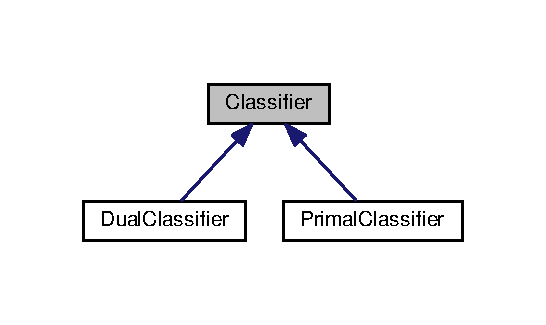
\includegraphics[width=350pt]{class_classifier__inherit__graph}
\end{center}
\end{figure}


Collaboration diagram for Classifier\+:\nopagebreak
\begin{figure}[H]
\begin{center}
\leavevmode
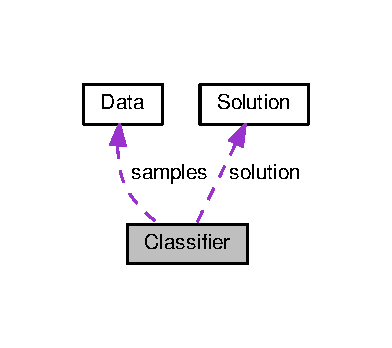
\includegraphics[width=188pt]{class_classifier__coll__graph}
\end{center}
\end{figure}
\subsection*{Public Member Functions}
\begin{DoxyCompactItemize}
\item 
virtual std\+::string \hyperlink{class_classifier_a7bfe7cc88b851b4a7e7ec55b30dd844e}{classifier\+Type} ()=0
\begin{DoxyCompactList}\small\item\em Returns the type of the classifier. \end{DoxyCompactList}\item 
virtual bool \hyperlink{class_classifier_a2306a5de27555ab093593ac9642bc7d9}{train} ()=0
\begin{DoxyCompactList}\small\item\em Function that execute the training phase of a classification algorithm. \end{DoxyCompactList}\item 
virtual double \hyperlink{class_classifier_ae8e9554823b85ddc2dcad2955da811d9}{evaluate} (\hyperlink{class_point}{Point} p)=0
\begin{DoxyCompactList}\small\item\em Returns the class of a feature point based on the trained classifier. \end{DoxyCompactList}\item 
virtual void \hyperlink{class_classifier_a4b16736670cba8f4c8397b6a90c8c799}{set\+Samples} (\hyperlink{class_data}{Data} $\ast$\hyperlink{class_classifier_a515c225d0da93df02ca79f9f87811d17}{samples})
\begin{DoxyCompactList}\small\item\em set\+Samples Set the samples used in the classifier. \end{DoxyCompactList}\item 
double \hyperlink{class_classifier_ab47b67b061041193aa3ae2a7856f4980}{get\+Elapsed\+Time} ()
\begin{DoxyCompactList}\small\item\em Get the elapsed time in the execution of the classifier. \end{DoxyCompactList}\item 
int \hyperlink{class_classifier_ab80a78cd6a4efc59b16f5b80cd64dc63}{get\+Ctot} ()
\begin{DoxyCompactList}\small\item\em Get the total number of updates of the classifier. \end{DoxyCompactList}\item 
int \hyperlink{class_classifier_a1fb3e4dfd80c154e89603c8fa1b11b76}{get\+Steps} ()
\begin{DoxyCompactList}\small\item\em get\+Steps Returns the number of steps through the data by the classifier. \end{DoxyCompactList}\item 
int \hyperlink{class_classifier_a738c2fbed982db6cad02062edcc037e4}{get\+Updates} ()
\begin{DoxyCompactList}\small\item\em get\+Updates Returns the number of updates needed to get to the the solution. \end{DoxyCompactList}\item 
void \hyperlink{class_classifier_a779b6cac0351e272ee0573d919d5d060}{set\+Steps} (int \hyperlink{class_classifier_a1e4c9c9ba059d5aff1d4d81eb41725cb}{steps})
\begin{DoxyCompactList}\small\item\em Set the partial number of steps of the classifier. \end{DoxyCompactList}\item 
void \hyperlink{class_classifier_a3293d7d39c3934503a23b920f84f73e7}{set\+Ctot} (int \hyperlink{class_classifier_a99d9a7f504212bb3dc2726c10a2333c6}{ctot})
\begin{DoxyCompactList}\small\item\em Set the partial number of updates of the classifier. \end{DoxyCompactList}\item 
void \hyperlink{class_classifier_a073b94029512378ccfae3aa34aae0212}{set\+Verbose} (int verbose)
\begin{DoxyCompactList}\small\item\em Set the level of verbose. \end{DoxyCompactList}\item 
void \hyperlink{class_classifier_a7f1cf3ac53b0593307a050368a912bb4}{set\+Start\+Time} (double \hyperlink{class_classifier_a4488a20bd7b4fc22d57244aaee57b002}{start\+\_\+time})
\begin{DoxyCompactList}\small\item\em set\+Start\+Time Set the initial time of the classifier. \end{DoxyCompactList}\item 
void \hyperlink{class_classifier_aef6cb633eed60712f8948a404f630e82}{set\+Solution} (\hyperlink{class_solution}{Solution} \hyperlink{class_classifier_a8e70651d36fa396f55028847acd6ae50}{solution})
\begin{DoxyCompactList}\small\item\em set\+Max\+Time Set the maximum time of the classifier. \end{DoxyCompactList}\item 
\hyperlink{class_solution}{Solution} \hyperlink{class_classifier_afd2b54ada10af9f4be1c4d326b180dc7}{get\+Solution} ()
\begin{DoxyCompactList}\small\item\em get\+Solution Returns the solution of the primal classifier. \end{DoxyCompactList}\item 
void \hyperlink{class_classifier_a5da324a0de94b7171484f3b1f1f22fbd}{set\+Max\+Time} (double \hyperlink{class_classifier_a191089f044af0f4dd51f37aaff78d8f6}{max\+\_\+time})
\begin{DoxyCompactList}\small\item\em Set the max time of execution. \end{DoxyCompactList}\item 
void \hyperlink{class_classifier_a9cc5a1d92243f9d9b530347be1ac7367}{set\+E\+PS} (double \hyperlink{class_classifier_ad7cd0cfea68461340df2adb0c132dc93}{E\+PS})
\begin{DoxyCompactList}\small\item\em set\+E\+PS Set the precision of the classifier. \end{DoxyCompactList}\item 
void \hyperlink{class_classifier_a58540f77a22c0f1774d0089fac713498}{set\+Max\+Iterations} (int \hyperlink{class_classifier_a9cab88ab4489d771256bffb1717c1644}{M\+A\+X\+\_\+\+IT})
\begin{DoxyCompactList}\small\item\em set\+Max\+Iterations Set the max number of iterations of the classifier. \end{DoxyCompactList}\item 
void \hyperlink{class_classifier_ad8930d5e6002299bdb840d4542229f02}{set\+Max\+Updates} (int \hyperlink{class_classifier_abb8b95854801151e78a1d9f6a2173c22}{M\+A\+X\+\_\+\+UP})
\begin{DoxyCompactList}\small\item\em set\+Max\+Iterations Set the max number of updates of the classifier. \end{DoxyCompactList}\item 
void \hyperlink{class_classifier_a8f6818bd403afbb46d1bfd75c9731ab6}{set\+Learning\+Rate} (double \hyperlink{class_classifier_af9867e5919742de1303dd971a9a1c19a}{rate})
\begin{DoxyCompactList}\small\item\em Set the learning rate of the classifier. \end{DoxyCompactList}\end{DoxyCompactItemize}
\subsection*{Protected Attributes}
\begin{DoxyCompactItemize}
\item 
\mbox{\Hypertarget{class_classifier_a1de0c258e4a175ebf96a18ec7ee33381}\label{class_classifier_a1de0c258e4a175ebf96a18ec7ee33381}} 
bool \hyperlink{class_classifier_a1de0c258e4a175ebf96a18ec7ee33381}{has\+Initial\+Solution} = false
\begin{DoxyCompactList}\small\item\em Inform if there\textquotesingle{}s an initial solution. \end{DoxyCompactList}\item 
\mbox{\Hypertarget{class_classifier_a515c225d0da93df02ca79f9f87811d17}\label{class_classifier_a515c225d0da93df02ca79f9f87811d17}} 
\hyperlink{class_data}{Data} $\ast$ \hyperlink{class_classifier_a515c225d0da93df02ca79f9f87811d17}{samples}
\begin{DoxyCompactList}\small\item\em Samples used in the model training. \end{DoxyCompactList}\item 
\mbox{\Hypertarget{class_classifier_ae9146fbbd020de483957a1ea68b614c7}\label{class_classifier_ae9146fbbd020de483957a1ea68b614c7}} 
std\+::vector$<$ \hyperlink{class_point}{Point} $>$ \hyperlink{class_classifier_ae9146fbbd020de483957a1ea68b614c7}{svs}
\begin{DoxyCompactList}\small\item\em Support vectors points. \end{DoxyCompactList}\item 
\mbox{\Hypertarget{class_classifier_a8e70651d36fa396f55028847acd6ae50}\label{class_classifier_a8e70651d36fa396f55028847acd6ae50}} 
\hyperlink{class_solution}{Solution} \hyperlink{class_classifier_a8e70651d36fa396f55028847acd6ae50}{solution}
\begin{DoxyCompactList}\small\item\em \hyperlink{class_classifier}{Classifier} solution. \end{DoxyCompactList}\item 
\mbox{\Hypertarget{class_classifier_af9867e5919742de1303dd971a9a1c19a}\label{class_classifier_af9867e5919742de1303dd971a9a1c19a}} 
double \hyperlink{class_classifier_af9867e5919742de1303dd971a9a1c19a}{rate} = 0.\+5f
\begin{DoxyCompactList}\small\item\em Learning rate. \end{DoxyCompactList}\item 
\mbox{\Hypertarget{class_classifier_a4488a20bd7b4fc22d57244aaee57b002}\label{class_classifier_a4488a20bd7b4fc22d57244aaee57b002}} 
double \hyperlink{class_classifier_a4488a20bd7b4fc22d57244aaee57b002}{start\+\_\+time} = 0.\+0f
\begin{DoxyCompactList}\small\item\em Initial time. \end{DoxyCompactList}\item 
\mbox{\Hypertarget{class_classifier_a191089f044af0f4dd51f37aaff78d8f6}\label{class_classifier_a191089f044af0f4dd51f37aaff78d8f6}} 
long int \hyperlink{class_classifier_a191089f044af0f4dd51f37aaff78d8f6}{max\+\_\+time} = 200
\begin{DoxyCompactList}\small\item\em Maximum time of training. \end{DoxyCompactList}\item 
\mbox{\Hypertarget{class_classifier_a1e4c9c9ba059d5aff1d4d81eb41725cb}\label{class_classifier_a1e4c9c9ba059d5aff1d4d81eb41725cb}} 
int \hyperlink{class_classifier_a1e4c9c9ba059d5aff1d4d81eb41725cb}{steps} = 0
\begin{DoxyCompactList}\small\item\em Number of steps in the data. \end{DoxyCompactList}\item 
\mbox{\Hypertarget{class_classifier_a99d9a7f504212bb3dc2726c10a2333c6}\label{class_classifier_a99d9a7f504212bb3dc2726c10a2333c6}} 
int \hyperlink{class_classifier_a99d9a7f504212bb3dc2726c10a2333c6}{ctot} = 0
\begin{DoxyCompactList}\small\item\em Number of updates of the weights. \end{DoxyCompactList}\item 
\mbox{\Hypertarget{class_classifier_ad7cd0cfea68461340df2adb0c132dc93}\label{class_classifier_ad7cd0cfea68461340df2adb0c132dc93}} 
double \hyperlink{class_classifier_ad7cd0cfea68461340df2adb0c132dc93}{E\+PS} = 1\+E-\/9
\begin{DoxyCompactList}\small\item\em Max precision. \end{DoxyCompactList}\item 
\mbox{\Hypertarget{class_classifier_a9cab88ab4489d771256bffb1717c1644}\label{class_classifier_a9cab88ab4489d771256bffb1717c1644}} 
int \hyperlink{class_classifier_a9cab88ab4489d771256bffb1717c1644}{M\+A\+X\+\_\+\+IT} = 1\+E9
\begin{DoxyCompactList}\small\item\em Max number of iterations. \end{DoxyCompactList}\item 
\mbox{\Hypertarget{class_classifier_abb8b95854801151e78a1d9f6a2173c22}\label{class_classifier_abb8b95854801151e78a1d9f6a2173c22}} 
int \hyperlink{class_classifier_abb8b95854801151e78a1d9f6a2173c22}{M\+A\+X\+\_\+\+UP} = 1\+E9
\begin{DoxyCompactList}\small\item\em Max number of updates. \end{DoxyCompactList}\item 
\mbox{\Hypertarget{class_classifier_a2b24f7f87ca8171ce07c888583646263}\label{class_classifier_a2b24f7f87ca8171ce07c888583646263}} 
int {\bfseries verbose} = 1
\item 
\mbox{\Hypertarget{class_classifier_ae9d28253495ae8807d586faff951d46f}\label{class_classifier_ae9d28253495ae8807d586faff951d46f}} 
\hyperlink{class_timer}{Timer} \hyperlink{class_classifier_ae9d28253495ae8807d586faff951d46f}{timer}
\begin{DoxyCompactList}\small\item\em \hyperlink{class_timer}{Timer} used to measure the time elapsed in the execution of classifier. \end{DoxyCompactList}\end{DoxyCompactItemize}


\subsection{Member Function Documentation}
\mbox{\Hypertarget{class_classifier_a7bfe7cc88b851b4a7e7ec55b30dd844e}\label{class_classifier_a7bfe7cc88b851b4a7e7ec55b30dd844e}} 
\index{Classifier@{Classifier}!classifier\+Type@{classifier\+Type}}
\index{classifier\+Type@{classifier\+Type}!Classifier@{Classifier}}
\subsubsection{\texorpdfstring{classifier\+Type()}{classifierType()}}
{\footnotesize\ttfamily virtual std\+::string Classifier\+::classifier\+Type (\begin{DoxyParamCaption}{ }\end{DoxyParamCaption})\hspace{0.3cm}{\ttfamily [pure virtual]}}



Returns the type of the classifier. 

\begin{DoxyReturn}{Returns}
std\+::string 
\end{DoxyReturn}


Implemented in \hyperlink{class_primal_classifier_af5117ae286ed7f06430b98f433e9bf62}{Primal\+Classifier}, and \hyperlink{class_dual_classifier_afbede25a3e30b87503c0c6555d52f358}{Dual\+Classifier}.

\mbox{\Hypertarget{class_classifier_ae8e9554823b85ddc2dcad2955da811d9}\label{class_classifier_ae8e9554823b85ddc2dcad2955da811d9}} 
\index{Classifier@{Classifier}!evaluate@{evaluate}}
\index{evaluate@{evaluate}!Classifier@{Classifier}}
\subsubsection{\texorpdfstring{evaluate()}{evaluate()}}
{\footnotesize\ttfamily virtual double Classifier\+::evaluate (\begin{DoxyParamCaption}\item[{\hyperlink{class_point}{Point}}]{p }\end{DoxyParamCaption})\hspace{0.3cm}{\ttfamily [pure virtual]}}



Returns the class of a feature point based on the trained classifier. 


\begin{DoxyParams}{Parameters}
{\em \hyperlink{class_point}{Point}} & x (???) Features point to be evaluated. \\
\hline
\end{DoxyParams}
\begin{DoxyReturn}{Returns}
int 
\end{DoxyReturn}


Implemented in \hyperlink{class_perceptron_fixed_margin_dual_a1370fdbc95bf728f82a83f219be32d23}{Perceptron\+Fixed\+Margin\+Dual}, \hyperlink{class_i_m_ap_fixed_margin_a230aae2c6ef3f70b2e1a704b5e4dff28}{I\+M\+Ap\+Fixed\+Margin}, \hyperlink{class_perceptron_dual_a3ed5554b85b4b1ec98f57acab3eeeaca}{Perceptron\+Dual}, \hyperlink{class_perceptron_fixed_margin_primal_af72c3dde96f1f1b803c7b522b5c1cc0f}{Perceptron\+Fixed\+Margin\+Primal}, \hyperlink{class_i_m_ap_aee497c8ff854b8d584c6c9df0c57ad57}{I\+M\+Ap}, and \hyperlink{class_perceptron_primal_ac8ce9ceffe2b35b5386e5367fb419b3b}{Perceptron\+Primal}.

\mbox{\Hypertarget{class_classifier_ab80a78cd6a4efc59b16f5b80cd64dc63}\label{class_classifier_ab80a78cd6a4efc59b16f5b80cd64dc63}} 
\index{Classifier@{Classifier}!get\+Ctot@{get\+Ctot}}
\index{get\+Ctot@{get\+Ctot}!Classifier@{Classifier}}
\subsubsection{\texorpdfstring{get\+Ctot()}{getCtot()}}
{\footnotesize\ttfamily int Classifier\+::get\+Ctot (\begin{DoxyParamCaption}{ }\end{DoxyParamCaption})\hspace{0.3cm}{\ttfamily [inline]}}



Get the total number of updates of the classifier. 

\begin{DoxyReturn}{Returns}
int 
\end{DoxyReturn}
\mbox{\Hypertarget{class_classifier_ab47b67b061041193aa3ae2a7856f4980}\label{class_classifier_ab47b67b061041193aa3ae2a7856f4980}} 
\index{Classifier@{Classifier}!get\+Elapsed\+Time@{get\+Elapsed\+Time}}
\index{get\+Elapsed\+Time@{get\+Elapsed\+Time}!Classifier@{Classifier}}
\subsubsection{\texorpdfstring{get\+Elapsed\+Time()}{getElapsedTime()}}
{\footnotesize\ttfamily double Classifier\+::get\+Elapsed\+Time (\begin{DoxyParamCaption}{ }\end{DoxyParamCaption})\hspace{0.3cm}{\ttfamily [inline]}}



Get the elapsed time in the execution of the classifier. 

\begin{DoxyReturn}{Returns}
double 
\end{DoxyReturn}
\mbox{\Hypertarget{class_classifier_afd2b54ada10af9f4be1c4d326b180dc7}\label{class_classifier_afd2b54ada10af9f4be1c4d326b180dc7}} 
\index{Classifier@{Classifier}!get\+Solution@{get\+Solution}}
\index{get\+Solution@{get\+Solution}!Classifier@{Classifier}}
\subsubsection{\texorpdfstring{get\+Solution()}{getSolution()}}
{\footnotesize\ttfamily \hyperlink{class_solution}{Solution} Classifier\+::get\+Solution (\begin{DoxyParamCaption}{ }\end{DoxyParamCaption})}



get\+Solution Returns the solution of the primal classifier. 

\begin{DoxyReturn}{Returns}
\hyperlink{class_solution}{Solution} 
\end{DoxyReturn}
\mbox{\Hypertarget{class_classifier_a1fb3e4dfd80c154e89603c8fa1b11b76}\label{class_classifier_a1fb3e4dfd80c154e89603c8fa1b11b76}} 
\index{Classifier@{Classifier}!get\+Steps@{get\+Steps}}
\index{get\+Steps@{get\+Steps}!Classifier@{Classifier}}
\subsubsection{\texorpdfstring{get\+Steps()}{getSteps()}}
{\footnotesize\ttfamily int Classifier\+::get\+Steps (\begin{DoxyParamCaption}{ }\end{DoxyParamCaption})\hspace{0.3cm}{\ttfamily [inline]}}



get\+Steps Returns the number of steps through the data by the classifier. 

\begin{DoxyReturn}{Returns}
int 
\end{DoxyReturn}
\mbox{\Hypertarget{class_classifier_a738c2fbed982db6cad02062edcc037e4}\label{class_classifier_a738c2fbed982db6cad02062edcc037e4}} 
\index{Classifier@{Classifier}!get\+Updates@{get\+Updates}}
\index{get\+Updates@{get\+Updates}!Classifier@{Classifier}}
\subsubsection{\texorpdfstring{get\+Updates()}{getUpdates()}}
{\footnotesize\ttfamily int Classifier\+::get\+Updates (\begin{DoxyParamCaption}{ }\end{DoxyParamCaption})\hspace{0.3cm}{\ttfamily [inline]}}



get\+Updates Returns the number of updates needed to get to the the solution. 

\begin{DoxyReturn}{Returns}
int 
\end{DoxyReturn}
\mbox{\Hypertarget{class_classifier_a3293d7d39c3934503a23b920f84f73e7}\label{class_classifier_a3293d7d39c3934503a23b920f84f73e7}} 
\index{Classifier@{Classifier}!set\+Ctot@{set\+Ctot}}
\index{set\+Ctot@{set\+Ctot}!Classifier@{Classifier}}
\subsubsection{\texorpdfstring{set\+Ctot()}{setCtot()}}
{\footnotesize\ttfamily void Classifier\+::set\+Ctot (\begin{DoxyParamCaption}\item[{int}]{ctot }\end{DoxyParamCaption})}



Set the partial number of updates of the classifier. 


\begin{DoxyParams}{Parameters}
{\em ctot} & Number of updates. \\
\hline
\end{DoxyParams}
\mbox{\Hypertarget{class_classifier_a9cc5a1d92243f9d9b530347be1ac7367}\label{class_classifier_a9cc5a1d92243f9d9b530347be1ac7367}} 
\index{Classifier@{Classifier}!set\+E\+PS@{set\+E\+PS}}
\index{set\+E\+PS@{set\+E\+PS}!Classifier@{Classifier}}
\subsubsection{\texorpdfstring{set\+E\+P\+S()}{setEPS()}}
{\footnotesize\ttfamily void Classifier\+::set\+E\+PS (\begin{DoxyParamCaption}\item[{double}]{E\+PS }\end{DoxyParamCaption})}



set\+E\+PS Set the precision of the classifier. 


\begin{DoxyParams}{Parameters}
{\em E\+PS} & Precision. \\
\hline
\end{DoxyParams}
\mbox{\Hypertarget{class_classifier_a8f6818bd403afbb46d1bfd75c9731ab6}\label{class_classifier_a8f6818bd403afbb46d1bfd75c9731ab6}} 
\index{Classifier@{Classifier}!set\+Learning\+Rate@{set\+Learning\+Rate}}
\index{set\+Learning\+Rate@{set\+Learning\+Rate}!Classifier@{Classifier}}
\subsubsection{\texorpdfstring{set\+Learning\+Rate()}{setLearningRate()}}
{\footnotesize\ttfamily void Classifier\+::set\+Learning\+Rate (\begin{DoxyParamCaption}\item[{double}]{rate }\end{DoxyParamCaption})}



Set the learning rate of the classifier. 


\begin{DoxyParams}{Parameters}
{\em rate} & Learning rate. \\
\hline
\end{DoxyParams}
\mbox{\Hypertarget{class_classifier_a58540f77a22c0f1774d0089fac713498}\label{class_classifier_a58540f77a22c0f1774d0089fac713498}} 
\index{Classifier@{Classifier}!set\+Max\+Iterations@{set\+Max\+Iterations}}
\index{set\+Max\+Iterations@{set\+Max\+Iterations}!Classifier@{Classifier}}
\subsubsection{\texorpdfstring{set\+Max\+Iterations()}{setMaxIterations()}}
{\footnotesize\ttfamily void Classifier\+::set\+Max\+Iterations (\begin{DoxyParamCaption}\item[{int}]{M\+A\+X\+\_\+\+IT }\end{DoxyParamCaption})}



set\+Max\+Iterations Set the max number of iterations of the classifier. 


\begin{DoxyParams}{Parameters}
{\em M\+A\+X\+\_\+\+IT} & Number max of iterations. \\
\hline
\end{DoxyParams}
\mbox{\Hypertarget{class_classifier_a5da324a0de94b7171484f3b1f1f22fbd}\label{class_classifier_a5da324a0de94b7171484f3b1f1f22fbd}} 
\index{Classifier@{Classifier}!set\+Max\+Time@{set\+Max\+Time}}
\index{set\+Max\+Time@{set\+Max\+Time}!Classifier@{Classifier}}
\subsubsection{\texorpdfstring{set\+Max\+Time()}{setMaxTime()}}
{\footnotesize\ttfamily void Classifier\+::set\+Max\+Time (\begin{DoxyParamCaption}\item[{double}]{max\+\_\+time }\end{DoxyParamCaption})}



Set the max time of execution. 


\begin{DoxyParams}{Parameters}
{\em max\+\_\+time} & Max time. \\
\hline
\end{DoxyParams}
\mbox{\Hypertarget{class_classifier_ad8930d5e6002299bdb840d4542229f02}\label{class_classifier_ad8930d5e6002299bdb840d4542229f02}} 
\index{Classifier@{Classifier}!set\+Max\+Updates@{set\+Max\+Updates}}
\index{set\+Max\+Updates@{set\+Max\+Updates}!Classifier@{Classifier}}
\subsubsection{\texorpdfstring{set\+Max\+Updates()}{setMaxUpdates()}}
{\footnotesize\ttfamily void Classifier\+::set\+Max\+Updates (\begin{DoxyParamCaption}\item[{int}]{M\+A\+X\+\_\+\+UP }\end{DoxyParamCaption})}



set\+Max\+Iterations Set the max number of updates of the classifier. 


\begin{DoxyParams}{Parameters}
{\em M\+A\+X\+\_\+\+IT} & Number max of updates. \\
\hline
\end{DoxyParams}
\mbox{\Hypertarget{class_classifier_a4b16736670cba8f4c8397b6a90c8c799}\label{class_classifier_a4b16736670cba8f4c8397b6a90c8c799}} 
\index{Classifier@{Classifier}!set\+Samples@{set\+Samples}}
\index{set\+Samples@{set\+Samples}!Classifier@{Classifier}}
\subsubsection{\texorpdfstring{set\+Samples()}{setSamples()}}
{\footnotesize\ttfamily void Classifier\+::set\+Samples (\begin{DoxyParamCaption}\item[{\hyperlink{class_data}{Data} $\ast$}]{samples }\end{DoxyParamCaption})\hspace{0.3cm}{\ttfamily [virtual]}}



set\+Samples Set the samples used in the classifier. 


\begin{DoxyParams}{Parameters}
{\em samples} & Samples to be used. \\
\hline
\end{DoxyParams}
\mbox{\Hypertarget{class_classifier_aef6cb633eed60712f8948a404f630e82}\label{class_classifier_aef6cb633eed60712f8948a404f630e82}} 
\index{Classifier@{Classifier}!set\+Solution@{set\+Solution}}
\index{set\+Solution@{set\+Solution}!Classifier@{Classifier}}
\subsubsection{\texorpdfstring{set\+Solution()}{setSolution()}}
{\footnotesize\ttfamily void Classifier\+::set\+Solution (\begin{DoxyParamCaption}\item[{\hyperlink{class_solution}{Solution}}]{solution }\end{DoxyParamCaption})}



set\+Max\+Time Set the maximum time of the classifier. 


\begin{DoxyParams}{Parameters}
{\em max\+\_\+time} & Maximum time. \\
\hline
\end{DoxyParams}
\mbox{\Hypertarget{class_classifier_a7f1cf3ac53b0593307a050368a912bb4}\label{class_classifier_a7f1cf3ac53b0593307a050368a912bb4}} 
\index{Classifier@{Classifier}!set\+Start\+Time@{set\+Start\+Time}}
\index{set\+Start\+Time@{set\+Start\+Time}!Classifier@{Classifier}}
\subsubsection{\texorpdfstring{set\+Start\+Time()}{setStartTime()}}
{\footnotesize\ttfamily void Classifier\+::set\+Start\+Time (\begin{DoxyParamCaption}\item[{double}]{start\+\_\+time }\end{DoxyParamCaption})}



set\+Start\+Time Set the initial time of the classifier. 


\begin{DoxyParams}{Parameters}
{\em start\+\_\+time} & Initial time. \\
\hline
\end{DoxyParams}
\mbox{\Hypertarget{class_classifier_a779b6cac0351e272ee0573d919d5d060}\label{class_classifier_a779b6cac0351e272ee0573d919d5d060}} 
\index{Classifier@{Classifier}!set\+Steps@{set\+Steps}}
\index{set\+Steps@{set\+Steps}!Classifier@{Classifier}}
\subsubsection{\texorpdfstring{set\+Steps()}{setSteps()}}
{\footnotesize\ttfamily void Classifier\+::set\+Steps (\begin{DoxyParamCaption}\item[{int}]{steps }\end{DoxyParamCaption})\hspace{0.3cm}{\ttfamily [inline]}}



Set the partial number of steps of the classifier. 


\begin{DoxyParams}{Parameters}
{\em steps} & Number of steps. \\
\hline
\end{DoxyParams}
\mbox{\Hypertarget{class_classifier_a073b94029512378ccfae3aa34aae0212}\label{class_classifier_a073b94029512378ccfae3aa34aae0212}} 
\index{Classifier@{Classifier}!set\+Verbose@{set\+Verbose}}
\index{set\+Verbose@{set\+Verbose}!Classifier@{Classifier}}
\subsubsection{\texorpdfstring{set\+Verbose()}{setVerbose()}}
{\footnotesize\ttfamily void Classifier\+::set\+Verbose (\begin{DoxyParamCaption}\item[{int}]{verbose }\end{DoxyParamCaption})}



Set the level of verbose. 


\begin{DoxyParams}{Parameters}
{\em verbose} & level of verbose. \\
\hline
\end{DoxyParams}
\mbox{\Hypertarget{class_classifier_a2306a5de27555ab093593ac9642bc7d9}\label{class_classifier_a2306a5de27555ab093593ac9642bc7d9}} 
\index{Classifier@{Classifier}!train@{train}}
\index{train@{train}!Classifier@{Classifier}}
\subsubsection{\texorpdfstring{train()}{train()}}
{\footnotesize\ttfamily virtual bool Classifier\+::train (\begin{DoxyParamCaption}{ }\end{DoxyParamCaption})\hspace{0.3cm}{\ttfamily [pure virtual]}}



Function that execute the training phase of a classification algorithm. 

\begin{DoxyReturn}{Returns}
void 
\end{DoxyReturn}


Implemented in \hyperlink{class_perceptron_fixed_margin_dual_aa095c90a3d04f70e1cf2e38e2afa769b}{Perceptron\+Fixed\+Margin\+Dual}, \hyperlink{class_i_m_ap_fixed_margin_ac43bc5733e6e749309277d3d99a86c11}{I\+M\+Ap\+Fixed\+Margin}, \hyperlink{class_perceptron_dual_a91b0bd1e86a6003b57b96199266cdc3e}{Perceptron\+Dual}, \hyperlink{class_perceptron_fixed_margin_primal_ad41c2a42c4a819c03bf9879110b0f99f}{Perceptron\+Fixed\+Margin\+Primal}, \hyperlink{class_i_m_ap_a6b6446fa6019518ae0336cb28af0b7f8}{I\+M\+Ap}, and \hyperlink{class_perceptron_primal_a17f817a72fc7d61d1686ea77f7f9e84d}{Perceptron\+Primal}.



The documentation for this class was generated from the following files\+:\begin{DoxyCompactItemize}
\item 
includes/Classifier.\+hpp\item 
src/Classifier.\+cpp\end{DoxyCompactItemize}

\hypertarget{class_data}{}\section{Data Class Reference}
\label{class_data}\index{Data@{Data}}


Wrapper for the dataset data.  




{\ttfamily \#include $<$Data.\+hpp$>$}

\subsection*{Public Member Functions}
\begin{DoxyCompactItemize}
\item 
\hyperlink{class_data_aa3ca35c963eec5a4734df23f88443077}{Data} (const char $\ast$pos\+\_\+class=\char`\"{}1\char`\"{}, const char $\ast$neg\+\_\+class=\char`\"{}-\/1\char`\"{})
\begin{DoxyCompactList}\small\item\em Constructor for empty data. \end{DoxyCompactList}\item 
\hyperlink{class_data_a85afba1f115dce4b6d2a952326624dd4}{Data} (std\+::string dataset, const char $\ast$pos\+\_\+class=\char`\"{}1\char`\"{}, const char $\ast$neg\+\_\+class=\char`\"{}-\/1\char`\"{})
\begin{DoxyCompactList}\small\item\em \hyperlink{class_data}{Data} constructor to load a dataset from a file. \end{DoxyCompactList}\item 
void \hyperlink{class_data_a6550f72555320ae9225ba216a9f4e7b3}{write} (std\+::string fname, std\+::string ext)
\begin{DoxyCompactList}\small\item\em write Write the data to a file with the given extention. \end{DoxyCompactList}\item 
int \hyperlink{class_data_abfd7c7cca66a186ff45efa430bcb2f1e}{get\+Size} ()
\begin{DoxyCompactList}\small\item\em Returns the size of the dataset. \end{DoxyCompactList}\item 
int \hyperlink{class_data_a0391940729a8023ea9b154132a854d35}{get\+Dim} ()
\begin{DoxyCompactList}\small\item\em Returns the dimension of the dataset. \end{DoxyCompactList}\item 
void \hyperlink{class_data_aeedfb7697a9b3e6fec681b991cb46daa}{set\+Dim} (int dim)
\begin{DoxyCompactList}\small\item\em set\+Dim Set the dimension of the points. \end{DoxyCompactList}\item 
std\+::shared\+\_\+ptr$<$ \hyperlink{class_point}{Point} $>$ \hyperlink{class_data_abd978f3708d705e972dc458b6e3fe791}{get\+Point} (int index)
\begin{DoxyCompactList}\small\item\em Returns the point with the given index. \end{DoxyCompactList}\item 
void \hyperlink{class_data_ad1f5969b33170e908334bd1ad6163b54}{set\+Point} (int index, std\+::shared\+\_\+ptr$<$ \hyperlink{class_point}{Point} $>$ p)
\begin{DoxyCompactList}\small\item\em set\+Point Set the point in a position of the data. \end{DoxyCompactList}\item 
std\+::vector$<$ std\+::shared\+\_\+ptr$<$ \hyperlink{class_point}{Point} $>$ $>$ \hyperlink{class_data_a9310e45321bca4335b8ab3031d343e16}{get\+Points} ()
\begin{DoxyCompactList}\small\item\em Returns the vector of Points of the sample. \end{DoxyCompactList}\item 
std\+::vector$<$ int $>$ \hyperlink{class_data_a2f6399baee6535e7f48250da54fbf00d}{get\+Features\+Names} ()
\begin{DoxyCompactList}\small\item\em Returns the features names. \end{DoxyCompactList}\item 
void \hyperlink{class_data_a2702b6464d7299c3b62e4eb4390fecd6}{set\+Features\+Names} (std\+::vector$<$ int $>$ fnames)
\begin{DoxyCompactList}\small\item\em set\+Features\+Names Set the name of the features of the data. \end{DoxyCompactList}\item 
\hyperlink{class_statistics}{Statistics} \hyperlink{class_data_a26376768a100f1999ef3ac15a2aa2a67}{get\+Statistics} ()
\begin{DoxyCompactList}\small\item\em Returns a class with the statistics info of the sample. \end{DoxyCompactList}\item 
std\+::vector$<$ int $>$ \hyperlink{class_data_a16685ae631c5bedc22c974980bc74c05}{get\+Index} ()
\begin{DoxyCompactList}\small\item\em Returns the vector of indexes. \end{DoxyCompactList}\item 
\mbox{\Hypertarget{class_data_ab2debdff651c70d26f84c9ac20f4dee6}\label{class_data_ab2debdff651c70d26f84c9ac20f4dee6}} 
void {\bfseries set\+Index} (std\+::vector$<$ int $>$ index)
\item 
int \hyperlink{class_data_a45a39ab2144bcdd0ac1aa67d7d08a6cc}{get\+Number\+Positive\+Points} ()
\begin{DoxyCompactList}\small\item\em Return the number of positive points. \end{DoxyCompactList}\item 
int \hyperlink{class_data_a5166e74e946c2dbac75f383d63f018ea}{get\+Number\+Negative\+Points} ()
\begin{DoxyCompactList}\small\item\em Return the number of negative points. \end{DoxyCompactList}\item 
void \hyperlink{class_data_a6dd8a8a1e1659c76e5716fc8a23a86e2}{set\+Classes} (std\+::string pos, std\+::string neg)
\begin{DoxyCompactList}\small\item\em set\+Classes Set the classes of the dataset. \end{DoxyCompactList}\item 
bool \hyperlink{class_data_a93468d3b8b2ce0f73e369e5de160534e}{is\+Empty} ()
\begin{DoxyCompactList}\small\item\em Returns if there\textquotesingle{}s a dataset loaded. \end{DoxyCompactList}\item 
bool \hyperlink{class_data_ad96fc8e9c5ec9e40b1dc6d9670eefe0c}{is\+Normalized} ()
\begin{DoxyCompactList}\small\item\em Returns if the dataset is normalized. \end{DoxyCompactList}\item 
bool \hyperlink{class_data_ac2ed251251be234c607f486e16902112}{load} (std\+::string file)
\begin{DoxyCompactList}\small\item\em Load a dataset from a file. \end{DoxyCompactList}\item 
\mbox{\Hypertarget{class_data_a44b749f64ffa35e034f9503fdec4917e}\label{class_data_a44b749f64ffa35e034f9503fdec4917e}} 
void \hyperlink{class_data_a44b749f64ffa35e034f9503fdec4917e}{clear} ()
\begin{DoxyCompactList}\small\item\em clear Clear the data. \end{DoxyCompactList}\item 
\hyperlink{class_data}{Data} \hyperlink{class_data_afb7687021aa7d5f1ecae464eee601710}{copy} ()
\begin{DoxyCompactList}\small\item\em Returns a copy of the data. \end{DoxyCompactList}\item 
void \hyperlink{class_data_a6454e835f570d10e7614ac237d6fdf79}{copy\+Zero} (const \hyperlink{class_data}{Data} \&other)
\begin{DoxyCompactList}\small\item\em Returns a copy of the data with zero points. \end{DoxyCompactList}\item 
void \hyperlink{class_data_a83c2a01ded98c4fad0b5b31538039046}{join} (\hyperlink{class_data}{Data} data)
\begin{DoxyCompactList}\small\item\em Merge one dataset with another. \end{DoxyCompactList}\item 
bool \hyperlink{class_data_abb6aade47d78a284301c32e82b2cbee2}{insert\+Point} (\hyperlink{class_data}{Data} sample, int id)
\begin{DoxyCompactList}\small\item\em Insert a point to the data from another sample. \end{DoxyCompactList}\item 
bool \hyperlink{class_data_a4dcec7d15085d451cf46a0459fab9f46}{insert\+Point} (std\+::shared\+\_\+ptr$<$ \hyperlink{class_point}{Point} $>$ p)
\begin{DoxyCompactList}\small\item\em Insert a point to the end of vector points. \end{DoxyCompactList}\item 
std\+::vector$<$ bool $>$ \hyperlink{class_data_a6cc376e614e5440061c66833e1c8d30a}{remove\+Points} (std\+::vector$<$ int $>$ ids)
\begin{DoxyCompactList}\small\item\em Remove several points from the sample. \end{DoxyCompactList}\item 
bool \hyperlink{class_data_ad927494a13a5018ff3644212d7234a03}{remove\+Point} (int pid)
\begin{DoxyCompactList}\small\item\em Remove a point from the data. \end{DoxyCompactList}\item 
\hyperlink{class_data}{Data} \hyperlink{class_data_a90e4e972afe7cfd622d4935299def743}{insert\+Features} (std\+::vector$<$ int $>$ ins\+\_\+feat)
\begin{DoxyCompactList}\small\item\em insert\+Features Returns \hyperlink{class_data}{Data} object with only features in array. \end{DoxyCompactList}\item 
bool \hyperlink{class_data_a0e0136f31687452ff10b489f8804ceb8}{remove\+Features} (std\+::vector$<$ int $>$ feats)
\begin{DoxyCompactList}\small\item\em Remove several features from the sample. \end{DoxyCompactList}\item 
void \hyperlink{class_data_a3e66e3dce7675bf2a1eded906e3d7912}{change\+X\+Vector} (std\+::vector$<$ int $>$ index)
\begin{DoxyCompactList}\small\item\em Change the x vector of a sample. \end{DoxyCompactList}\item 
void \hyperlink{class_data_a38bbab57bd9d871bd78771df47529d6b}{normalize} (double p=2)
\begin{DoxyCompactList}\small\item\em normalize Normalize the dataset using a Lp-\/norm. \end{DoxyCompactList}\item 
\mbox{\Hypertarget{class_data_a02affbc0f8564106c84dc59f34666912}\label{class_data_a02affbc0f8564106c84dc59f34666912}} 
void {\bfseries operator=} (const \hyperlink{class_data}{Data} \&)
\end{DoxyCompactItemize}
\subsection*{Static Public Member Functions}
\begin{DoxyCompactItemize}
\item 
static void \hyperlink{class_data_acd8fd65a56a3d097d1bc19fb8249ee20}{normalize} (std\+::vector$<$ double $>$ \&p, double q)
\begin{DoxyCompactList}\small\item\em normalize Normalize a vector using a Lp-\/norm. \end{DoxyCompactList}\end{DoxyCompactItemize}
\subsection*{Friends}
\begin{DoxyCompactItemize}
\item 
\mbox{\Hypertarget{class_data_ae7387779a206ec9f8d282b354e0c3316}\label{class_data_ae7387779a206ec9f8d282b354e0c3316}} 
std\+::ostream \& {\bfseries operator$<$$<$} (std\+::ostream \&output, const \hyperlink{class_data}{Data} \&data)
\end{DoxyCompactItemize}


\subsection{Detailed Description}
Wrapper for the dataset data. 

\subsection{Constructor \& Destructor Documentation}
\mbox{\Hypertarget{class_data_aa3ca35c963eec5a4734df23f88443077}\label{class_data_aa3ca35c963eec5a4734df23f88443077}} 
\index{Data@{Data}!Data@{Data}}
\index{Data@{Data}!Data@{Data}}
\subsubsection{\texorpdfstring{Data()}{Data()}\hspace{0.1cm}{\footnotesize\ttfamily [1/2]}}
{\footnotesize\ttfamily Data\+::\+Data (\begin{DoxyParamCaption}\item[{const char $\ast$}]{pos\+\_\+class = {\ttfamily \char`\"{}1\char`\"{}},  }\item[{const char $\ast$}]{neg\+\_\+class = {\ttfamily \char`\"{}-\/1\char`\"{}} }\end{DoxyParamCaption})}



Constructor for empty data. 


\begin{DoxyParams}{Parameters}
{\em pos\+\_\+class} & String representing the positive class on the dataset. \\
\hline
{\em neg\+\_\+class} & String representing the negative class on the dataset. \\
\hline
\end{DoxyParams}
\mbox{\Hypertarget{class_data_a85afba1f115dce4b6d2a952326624dd4}\label{class_data_a85afba1f115dce4b6d2a952326624dd4}} 
\index{Data@{Data}!Data@{Data}}
\index{Data@{Data}!Data@{Data}}
\subsubsection{\texorpdfstring{Data()}{Data()}\hspace{0.1cm}{\footnotesize\ttfamily [2/2]}}
{\footnotesize\ttfamily Data\+::\+Data (\begin{DoxyParamCaption}\item[{std\+::string}]{dataset,  }\item[{const char $\ast$}]{pos\+\_\+class = {\ttfamily \char`\"{}1\char`\"{}},  }\item[{const char $\ast$}]{neg\+\_\+class = {\ttfamily \char`\"{}-\/1\char`\"{}} }\end{DoxyParamCaption})}



\hyperlink{class_data}{Data} constructor to load a dataset from a file. 


\begin{DoxyParams}{Parameters}
{\em dataset} & (???) Path to the dataset to be loaded. \\
\hline
{\em pos\+\_\+class} & String representing the positive class on the dataset. \\
\hline
{\em neg\+\_\+class} & String representing the negative class on the dataset. \\
\hline
\end{DoxyParams}


\subsection{Member Function Documentation}
\mbox{\Hypertarget{class_data_a3e66e3dce7675bf2a1eded906e3d7912}\label{class_data_a3e66e3dce7675bf2a1eded906e3d7912}} 
\index{Data@{Data}!change\+X\+Vector@{change\+X\+Vector}}
\index{change\+X\+Vector@{change\+X\+Vector}!Data@{Data}}
\subsubsection{\texorpdfstring{change\+X\+Vector()}{changeXVector()}}
{\footnotesize\ttfamily void Data\+::change\+X\+Vector (\begin{DoxyParamCaption}\item[{std\+::vector$<$ int $>$}]{index }\end{DoxyParamCaption})}



Change the x vector of a sample. 


\begin{DoxyParams}{Parameters}
{\em index} & (???) Indexes of the change to be made. \\
\hline
\end{DoxyParams}
\begin{DoxyReturn}{Returns}
void 
\end{DoxyReturn}
\mbox{\Hypertarget{class_data_afb7687021aa7d5f1ecae464eee601710}\label{class_data_afb7687021aa7d5f1ecae464eee601710}} 
\index{Data@{Data}!copy@{copy}}
\index{copy@{copy}!Data@{Data}}
\subsubsection{\texorpdfstring{copy()}{copy()}}
{\footnotesize\ttfamily \hyperlink{class_data}{Data} Data\+::copy (\begin{DoxyParamCaption}{ }\end{DoxyParamCaption})}



Returns a copy of the data. 

\begin{DoxyReturn}{Returns}
\hyperlink{class_data}{Data} 
\end{DoxyReturn}
\mbox{\Hypertarget{class_data_a6454e835f570d10e7614ac237d6fdf79}\label{class_data_a6454e835f570d10e7614ac237d6fdf79}} 
\index{Data@{Data}!copy\+Zero@{copy\+Zero}}
\index{copy\+Zero@{copy\+Zero}!Data@{Data}}
\subsubsection{\texorpdfstring{copy\+Zero()}{copyZero()}}
{\footnotesize\ttfamily void Data\+::copy\+Zero (\begin{DoxyParamCaption}\item[{const \hyperlink{class_data}{Data} \&}]{other }\end{DoxyParamCaption})}



Returns a copy of the data with zero points. 

\begin{DoxyReturn}{Returns}
\hyperlink{class_data}{Data} 
\end{DoxyReturn}
\mbox{\Hypertarget{class_data_a0391940729a8023ea9b154132a854d35}\label{class_data_a0391940729a8023ea9b154132a854d35}} 
\index{Data@{Data}!get\+Dim@{get\+Dim}}
\index{get\+Dim@{get\+Dim}!Data@{Data}}
\subsubsection{\texorpdfstring{get\+Dim()}{getDim()}}
{\footnotesize\ttfamily int Data\+::get\+Dim (\begin{DoxyParamCaption}{ }\end{DoxyParamCaption})}



Returns the dimension of the dataset. 

\begin{DoxyReturn}{Returns}
int 
\end{DoxyReturn}
\mbox{\Hypertarget{class_data_a2f6399baee6535e7f48250da54fbf00d}\label{class_data_a2f6399baee6535e7f48250da54fbf00d}} 
\index{Data@{Data}!get\+Features\+Names@{get\+Features\+Names}}
\index{get\+Features\+Names@{get\+Features\+Names}!Data@{Data}}
\subsubsection{\texorpdfstring{get\+Features\+Names()}{getFeaturesNames()}}
{\footnotesize\ttfamily vector$<$ int $>$ Data\+::get\+Features\+Names (\begin{DoxyParamCaption}{ }\end{DoxyParamCaption})}



Returns the features names. 

\begin{DoxyReturn}{Returns}
std\+::vector$<$int$>$ 
\end{DoxyReturn}
\mbox{\Hypertarget{class_data_a16685ae631c5bedc22c974980bc74c05}\label{class_data_a16685ae631c5bedc22c974980bc74c05}} 
\index{Data@{Data}!get\+Index@{get\+Index}}
\index{get\+Index@{get\+Index}!Data@{Data}}
\subsubsection{\texorpdfstring{get\+Index()}{getIndex()}}
{\footnotesize\ttfamily vector$<$ int $>$ Data\+::get\+Index (\begin{DoxyParamCaption}{ }\end{DoxyParamCaption})}



Returns the vector of indexes. 

\begin{DoxyReturn}{Returns}
std\+::vector$<$int$>$ 
\end{DoxyReturn}
\mbox{\Hypertarget{class_data_a5166e74e946c2dbac75f383d63f018ea}\label{class_data_a5166e74e946c2dbac75f383d63f018ea}} 
\index{Data@{Data}!get\+Number\+Negative\+Points@{get\+Number\+Negative\+Points}}
\index{get\+Number\+Negative\+Points@{get\+Number\+Negative\+Points}!Data@{Data}}
\subsubsection{\texorpdfstring{get\+Number\+Negative\+Points()}{getNumberNegativePoints()}}
{\footnotesize\ttfamily int Data\+::get\+Number\+Negative\+Points (\begin{DoxyParamCaption}{ }\end{DoxyParamCaption})}



Return the number of negative points. 

\begin{DoxyReturn}{Returns}
int 
\end{DoxyReturn}
\mbox{\Hypertarget{class_data_a45a39ab2144bcdd0ac1aa67d7d08a6cc}\label{class_data_a45a39ab2144bcdd0ac1aa67d7d08a6cc}} 
\index{Data@{Data}!get\+Number\+Positive\+Points@{get\+Number\+Positive\+Points}}
\index{get\+Number\+Positive\+Points@{get\+Number\+Positive\+Points}!Data@{Data}}
\subsubsection{\texorpdfstring{get\+Number\+Positive\+Points()}{getNumberPositivePoints()}}
{\footnotesize\ttfamily int Data\+::get\+Number\+Positive\+Points (\begin{DoxyParamCaption}{ }\end{DoxyParamCaption})}



Return the number of positive points. 

\begin{DoxyReturn}{Returns}
int 
\end{DoxyReturn}
\mbox{\Hypertarget{class_data_abd978f3708d705e972dc458b6e3fe791}\label{class_data_abd978f3708d705e972dc458b6e3fe791}} 
\index{Data@{Data}!get\+Point@{get\+Point}}
\index{get\+Point@{get\+Point}!Data@{Data}}
\subsubsection{\texorpdfstring{get\+Point()}{getPoint()}}
{\footnotesize\ttfamily shared\+\_\+ptr$<$ \hyperlink{class_point}{Point} $>$ Data\+::get\+Point (\begin{DoxyParamCaption}\item[{int}]{index }\end{DoxyParamCaption})}



Returns the point with the given index. 


\begin{DoxyParams}{Parameters}
{\em index} & Position of a point in the points array. \\
\hline
\end{DoxyParams}
\begin{DoxyReturn}{Returns}
std\+::vector$<$\+Points$>$ 
\end{DoxyReturn}
\mbox{\Hypertarget{class_data_a9310e45321bca4335b8ab3031d343e16}\label{class_data_a9310e45321bca4335b8ab3031d343e16}} 
\index{Data@{Data}!get\+Points@{get\+Points}}
\index{get\+Points@{get\+Points}!Data@{Data}}
\subsubsection{\texorpdfstring{get\+Points()}{getPoints()}}
{\footnotesize\ttfamily vector$<$ shared\+\_\+ptr$<$ \hyperlink{class_point}{Point} $>$ $>$ Data\+::get\+Points (\begin{DoxyParamCaption}{ }\end{DoxyParamCaption})}



Returns the vector of Points of the sample. 

\begin{DoxyReturn}{Returns}
std\+::vector$<$\+Points$>$ 
\end{DoxyReturn}
\mbox{\Hypertarget{class_data_abfd7c7cca66a186ff45efa430bcb2f1e}\label{class_data_abfd7c7cca66a186ff45efa430bcb2f1e}} 
\index{Data@{Data}!get\+Size@{get\+Size}}
\index{get\+Size@{get\+Size}!Data@{Data}}
\subsubsection{\texorpdfstring{get\+Size()}{getSize()}}
{\footnotesize\ttfamily int Data\+::get\+Size (\begin{DoxyParamCaption}{ }\end{DoxyParamCaption})}



Returns the size of the dataset. 

\begin{DoxyReturn}{Returns}
int 
\end{DoxyReturn}
\mbox{\Hypertarget{class_data_a26376768a100f1999ef3ac15a2aa2a67}\label{class_data_a26376768a100f1999ef3ac15a2aa2a67}} 
\index{Data@{Data}!get\+Statistics@{get\+Statistics}}
\index{get\+Statistics@{get\+Statistics}!Data@{Data}}
\subsubsection{\texorpdfstring{get\+Statistics()}{getStatistics()}}
{\footnotesize\ttfamily \hyperlink{class_statistics}{Statistics} Data\+::get\+Statistics (\begin{DoxyParamCaption}{ }\end{DoxyParamCaption})}



Returns a class with the statistics info of the sample. 

\begin{DoxyReturn}{Returns}
\hyperlink{class_statistics}{Statistics} 
\end{DoxyReturn}
\mbox{\Hypertarget{class_data_a90e4e972afe7cfd622d4935299def743}\label{class_data_a90e4e972afe7cfd622d4935299def743}} 
\index{Data@{Data}!insert\+Features@{insert\+Features}}
\index{insert\+Features@{insert\+Features}!Data@{Data}}
\subsubsection{\texorpdfstring{insert\+Features()}{insertFeatures()}}
{\footnotesize\ttfamily \hyperlink{class_data}{Data} Data\+::insert\+Features (\begin{DoxyParamCaption}\item[{std\+::vector$<$ int $>$}]{ins\+\_\+feat }\end{DoxyParamCaption})}



insert\+Features Returns \hyperlink{class_data}{Data} object with only features in array. 


\begin{DoxyParams}{Parameters}
{\em ins\+\_\+feat} & (???) Array with features that will be in the \hyperlink{class_data}{Data} object. \\
\hline
\end{DoxyParams}
\begin{DoxyReturn}{Returns}
\hyperlink{class_data}{Data} If the object is empty something wrong happened. 
\end{DoxyReturn}
\mbox{\Hypertarget{class_data_abb6aade47d78a284301c32e82b2cbee2}\label{class_data_abb6aade47d78a284301c32e82b2cbee2}} 
\index{Data@{Data}!insert\+Point@{insert\+Point}}
\index{insert\+Point@{insert\+Point}!Data@{Data}}
\subsubsection{\texorpdfstring{insert\+Point()}{insertPoint()}\hspace{0.1cm}{\footnotesize\ttfamily [1/2]}}
{\footnotesize\ttfamily bool Data\+::insert\+Point (\begin{DoxyParamCaption}\item[{\hyperlink{class_data}{Data}}]{sample,  }\item[{int}]{id }\end{DoxyParamCaption})}



Insert a point to the data from another sample. 


\begin{DoxyParams}{Parameters}
{\em sample} & (???) Sample with the point to be added. \\
\hline
{\em id} & (???) Index of the point to be added. \\
\hline
\end{DoxyParams}
\begin{DoxyReturn}{Returns}
bool 
\end{DoxyReturn}
\mbox{\Hypertarget{class_data_a4dcec7d15085d451cf46a0459fab9f46}\label{class_data_a4dcec7d15085d451cf46a0459fab9f46}} 
\index{Data@{Data}!insert\+Point@{insert\+Point}}
\index{insert\+Point@{insert\+Point}!Data@{Data}}
\subsubsection{\texorpdfstring{insert\+Point()}{insertPoint()}\hspace{0.1cm}{\footnotesize\ttfamily [2/2]}}
{\footnotesize\ttfamily bool Data\+::insert\+Point (\begin{DoxyParamCaption}\item[{std\+::shared\+\_\+ptr$<$ \hyperlink{class_point}{Point} $>$}]{p }\end{DoxyParamCaption})}



Insert a point to the end of vector points. 


\begin{DoxyParams}{Parameters}
{\em p} & (???) \hyperlink{class_point}{Point} to be inserted. \\
\hline
\end{DoxyParams}
\begin{DoxyReturn}{Returns}
bool 
\end{DoxyReturn}
\mbox{\Hypertarget{class_data_a93468d3b8b2ce0f73e369e5de160534e}\label{class_data_a93468d3b8b2ce0f73e369e5de160534e}} 
\index{Data@{Data}!is\+Empty@{is\+Empty}}
\index{is\+Empty@{is\+Empty}!Data@{Data}}
\subsubsection{\texorpdfstring{is\+Empty()}{isEmpty()}}
{\footnotesize\ttfamily bool Data\+::is\+Empty (\begin{DoxyParamCaption}{ }\end{DoxyParamCaption})}



Returns if there\textquotesingle{}s a dataset loaded. 

\begin{DoxyReturn}{Returns}
bool 
\end{DoxyReturn}
\mbox{\Hypertarget{class_data_ad96fc8e9c5ec9e40b1dc6d9670eefe0c}\label{class_data_ad96fc8e9c5ec9e40b1dc6d9670eefe0c}} 
\index{Data@{Data}!is\+Normalized@{is\+Normalized}}
\index{is\+Normalized@{is\+Normalized}!Data@{Data}}
\subsubsection{\texorpdfstring{is\+Normalized()}{isNormalized()}}
{\footnotesize\ttfamily bool Data\+::is\+Normalized (\begin{DoxyParamCaption}{ }\end{DoxyParamCaption})\hspace{0.3cm}{\ttfamily [inline]}}



Returns if the dataset is normalized. 

\begin{DoxyReturn}{Returns}
bool 
\end{DoxyReturn}
\mbox{\Hypertarget{class_data_a83c2a01ded98c4fad0b5b31538039046}\label{class_data_a83c2a01ded98c4fad0b5b31538039046}} 
\index{Data@{Data}!join@{join}}
\index{join@{join}!Data@{Data}}
\subsubsection{\texorpdfstring{join()}{join()}}
{\footnotesize\ttfamily void Data\+::join (\begin{DoxyParamCaption}\item[{\hyperlink{class_data}{Data}}]{data }\end{DoxyParamCaption})}



Merge one dataset with another. 


\begin{DoxyParams}{Parameters}
{\em data} & (???) Dataset to be joined. \\
\hline
\end{DoxyParams}
\begin{DoxyReturn}{Returns}
bool 
\end{DoxyReturn}
\mbox{\Hypertarget{class_data_ac2ed251251be234c607f486e16902112}\label{class_data_ac2ed251251be234c607f486e16902112}} 
\index{Data@{Data}!load@{load}}
\index{load@{load}!Data@{Data}}
\subsubsection{\texorpdfstring{load()}{load()}}
{\footnotesize\ttfamily bool Data\+::load (\begin{DoxyParamCaption}\item[{std\+::string}]{file }\end{DoxyParamCaption})}



Load a dataset from a file. 


\begin{DoxyParams}{Parameters}
{\em file} & (???) Path to dataset file. \\
\hline
\end{DoxyParams}
\begin{DoxyReturn}{Returns}
bool 
\end{DoxyReturn}
\mbox{\Hypertarget{class_data_a38bbab57bd9d871bd78771df47529d6b}\label{class_data_a38bbab57bd9d871bd78771df47529d6b}} 
\index{Data@{Data}!normalize@{normalize}}
\index{normalize@{normalize}!Data@{Data}}
\subsubsection{\texorpdfstring{normalize()}{normalize()}\hspace{0.1cm}{\footnotesize\ttfamily [1/2]}}
{\footnotesize\ttfamily void Data\+::normalize (\begin{DoxyParamCaption}\item[{double}]{p = {\ttfamily 2} }\end{DoxyParamCaption})}



normalize Normalize the dataset using a Lp-\/norm. 


\begin{DoxyParams}{Parameters}
{\em p} & Norm to be utilized. \\
\hline
\end{DoxyParams}
\mbox{\Hypertarget{class_data_acd8fd65a56a3d097d1bc19fb8249ee20}\label{class_data_acd8fd65a56a3d097d1bc19fb8249ee20}} 
\index{Data@{Data}!normalize@{normalize}}
\index{normalize@{normalize}!Data@{Data}}
\subsubsection{\texorpdfstring{normalize()}{normalize()}\hspace{0.1cm}{\footnotesize\ttfamily [2/2]}}
{\footnotesize\ttfamily static void Data\+::normalize (\begin{DoxyParamCaption}\item[{std\+::vector$<$ double $>$ \&}]{p,  }\item[{double}]{q }\end{DoxyParamCaption})\hspace{0.3cm}{\ttfamily [static]}}



normalize Normalize a vector using a Lp-\/norm. 


\begin{DoxyParams}{Parameters}
{\em q} & Norm to be utilized. \\
\hline
{\em p} & Vector to be normalized. \\
\hline
\end{DoxyParams}
\mbox{\Hypertarget{class_data_a0e0136f31687452ff10b489f8804ceb8}\label{class_data_a0e0136f31687452ff10b489f8804ceb8}} 
\index{Data@{Data}!remove\+Features@{remove\+Features}}
\index{remove\+Features@{remove\+Features}!Data@{Data}}
\subsubsection{\texorpdfstring{remove\+Features()}{removeFeatures()}}
{\footnotesize\ttfamily bool Data\+::remove\+Features (\begin{DoxyParamCaption}\item[{std\+::vector$<$ int $>$}]{feats }\end{DoxyParamCaption})}



Remove several features from the sample. 


\begin{DoxyParams}{Parameters}
{\em feats} & (???) Names of the features to be removed (must be sorted). \\
\hline
\end{DoxyParams}
\begin{DoxyReturn}{Returns}
boolean informing if all features were succesfully removed. 
\end{DoxyReturn}
\mbox{\Hypertarget{class_data_ad927494a13a5018ff3644212d7234a03}\label{class_data_ad927494a13a5018ff3644212d7234a03}} 
\index{Data@{Data}!remove\+Point@{remove\+Point}}
\index{remove\+Point@{remove\+Point}!Data@{Data}}
\subsubsection{\texorpdfstring{remove\+Point()}{removePoint()}}
{\footnotesize\ttfamily bool Data\+::remove\+Point (\begin{DoxyParamCaption}\item[{int}]{pid }\end{DoxyParamCaption})}



Remove a point from the data. 


\begin{DoxyParams}{Parameters}
{\em pid} & (???) Index of the point to be removed. \\
\hline
\end{DoxyParams}
\begin{DoxyReturn}{Returns}
bool 
\end{DoxyReturn}
\mbox{\Hypertarget{class_data_a6cc376e614e5440061c66833e1c8d30a}\label{class_data_a6cc376e614e5440061c66833e1c8d30a}} 
\index{Data@{Data}!remove\+Points@{remove\+Points}}
\index{remove\+Points@{remove\+Points}!Data@{Data}}
\subsubsection{\texorpdfstring{remove\+Points()}{removePoints()}}
{\footnotesize\ttfamily vector$<$ bool $>$ Data\+::remove\+Points (\begin{DoxyParamCaption}\item[{std\+::vector$<$ int $>$}]{ids }\end{DoxyParamCaption})}



Remove several points from the sample. 


\begin{DoxyParams}{Parameters}
{\em ids} & (???) Ids of the points to be removed (must be sorted). \\
\hline
\end{DoxyParams}
\begin{DoxyReturn}{Returns}
booleans informing which points were removed succesfully. 
\end{DoxyReturn}
\mbox{\Hypertarget{class_data_a6dd8a8a1e1659c76e5716fc8a23a86e2}\label{class_data_a6dd8a8a1e1659c76e5716fc8a23a86e2}} 
\index{Data@{Data}!set\+Classes@{set\+Classes}}
\index{set\+Classes@{set\+Classes}!Data@{Data}}
\subsubsection{\texorpdfstring{set\+Classes()}{setClasses()}}
{\footnotesize\ttfamily void Data\+::set\+Classes (\begin{DoxyParamCaption}\item[{std\+::string}]{pos,  }\item[{std\+::string}]{neg }\end{DoxyParamCaption})}



set\+Classes Set the classes of the dataset. 


\begin{DoxyParams}{Parameters}
{\em pos} & Positive class. \\
\hline
{\em neg} & Negative class. \\
\hline
\end{DoxyParams}
\mbox{\Hypertarget{class_data_aeedfb7697a9b3e6fec681b991cb46daa}\label{class_data_aeedfb7697a9b3e6fec681b991cb46daa}} 
\index{Data@{Data}!set\+Dim@{set\+Dim}}
\index{set\+Dim@{set\+Dim}!Data@{Data}}
\subsubsection{\texorpdfstring{set\+Dim()}{setDim()}}
{\footnotesize\ttfamily void Data\+::set\+Dim (\begin{DoxyParamCaption}\item[{int}]{dim }\end{DoxyParamCaption})}



set\+Dim Set the dimension of the points. 


\begin{DoxyParams}{Parameters}
{\em dim} & (???) Dimension to be set. \\
\hline
\end{DoxyParams}
\mbox{\Hypertarget{class_data_a2702b6464d7299c3b62e4eb4390fecd6}\label{class_data_a2702b6464d7299c3b62e4eb4390fecd6}} 
\index{Data@{Data}!set\+Features\+Names@{set\+Features\+Names}}
\index{set\+Features\+Names@{set\+Features\+Names}!Data@{Data}}
\subsubsection{\texorpdfstring{set\+Features\+Names()}{setFeaturesNames()}}
{\footnotesize\ttfamily void Data\+::set\+Features\+Names (\begin{DoxyParamCaption}\item[{std\+::vector$<$ int $>$}]{fnames }\end{DoxyParamCaption})}



set\+Features\+Names Set the name of the features of the data. 


\begin{DoxyParams}{Parameters}
{\em fnames} & (???) Name of the features. \\
\hline
\end{DoxyParams}
\mbox{\Hypertarget{class_data_ad1f5969b33170e908334bd1ad6163b54}\label{class_data_ad1f5969b33170e908334bd1ad6163b54}} 
\index{Data@{Data}!set\+Point@{set\+Point}}
\index{set\+Point@{set\+Point}!Data@{Data}}
\subsubsection{\texorpdfstring{set\+Point()}{setPoint()}}
{\footnotesize\ttfamily void Data\+::set\+Point (\begin{DoxyParamCaption}\item[{int}]{index,  }\item[{std\+::shared\+\_\+ptr$<$ \hyperlink{class_point}{Point} $>$}]{p }\end{DoxyParamCaption})}



set\+Point Set the point in a position of the data. 


\begin{DoxyParams}{Parameters}
{\em index} & (???) Index of the point that will be set. \\
\hline
{\em p} & (???) \hyperlink{class_point}{Point} to be set. \\
\hline
\end{DoxyParams}
\mbox{\Hypertarget{class_data_a6550f72555320ae9225ba216a9f4e7b3}\label{class_data_a6550f72555320ae9225ba216a9f4e7b3}} 
\index{Data@{Data}!write@{write}}
\index{write@{write}!Data@{Data}}
\subsubsection{\texorpdfstring{write()}{write()}}
{\footnotesize\ttfamily void Data\+::write (\begin{DoxyParamCaption}\item[{std\+::string}]{fname,  }\item[{std\+::string}]{ext }\end{DoxyParamCaption})}



write Write the data to a file with the given extention. 


\begin{DoxyParams}{Parameters}
{\em fname} & Name of the file. \\
\hline
{\em ext} & Extention of the file. \\
\hline
\end{DoxyParams}


The documentation for this class was generated from the following files\+:\begin{DoxyCompactItemize}
\item 
includes/Data.\+hpp\item 
src/\hyperlink{_data_8cpp}{Data.\+cpp}\end{DoxyCompactItemize}

\hypertarget{class_dual_classifier}{}\section{Dual\+Classifier Class Reference}
\label{class_dual_classifier}\index{Dual\+Classifier@{Dual\+Classifier}}


Inheritance diagram for Dual\+Classifier\+:\nopagebreak
\begin{figure}[H]
\begin{center}
\leavevmode
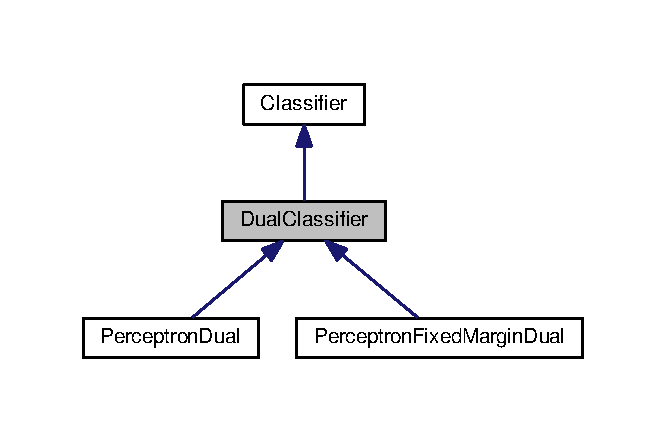
\includegraphics[width=320pt]{class_dual_classifier__inherit__graph}
\end{center}
\end{figure}


Collaboration diagram for Dual\+Classifier\+:\nopagebreak
\begin{figure}[H]
\begin{center}
\leavevmode
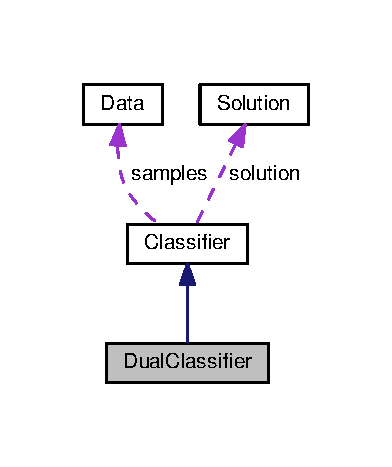
\includegraphics[width=246pt]{class_dual_classifier__coll__graph}
\end{center}
\end{figure}
\subsection*{Public Member Functions}
\begin{DoxyCompactItemize}
\item 
std\+::string \hyperlink{class_dual_classifier_afbede25a3e30b87503c0c6555d52f358}{classifier\+Type} ()
\begin{DoxyCompactList}\small\item\em Returns the type of the classifier. \end{DoxyCompactList}\item 
void \hyperlink{class_dual_classifier_a0cf616ad02cfcdd69cfd3d0b35001946}{set\+Kernel} (\hyperlink{class_kernel}{Kernel} K)
\begin{DoxyCompactList}\small\item\em set\+Kernel Set the kernel used by the dual classifier. \end{DoxyCompactList}\item 
double \hyperlink{class_dual_classifier_a5738038f99450f5f3b7098d3125ffaae}{get\+Kernel\+Param} ()
\begin{DoxyCompactList}\small\item\em Get the parameter of the kernel. \end{DoxyCompactList}\item 
double \hyperlink{class_dual_classifier_a14b35e85dddac38e7927cd03037e2353}{get\+Kernel\+Type} ()
\begin{DoxyCompactList}\small\item\em Get the type of the kernel. \end{DoxyCompactList}\end{DoxyCompactItemize}
\subsection*{Protected Attributes}
\begin{DoxyCompactItemize}
\item 
\mbox{\Hypertarget{class_dual_classifier_a0ed1219ed410852620b844934a8c70a0}\label{class_dual_classifier_a0ed1219ed410852620b844934a8c70a0}} 
std\+::vector$<$ double $>$ \hyperlink{class_dual_classifier_a0ed1219ed410852620b844934a8c70a0}{alpha}
\begin{DoxyCompactList}\small\item\em Alphas vector. \end{DoxyCompactList}\item 
\mbox{\Hypertarget{class_dual_classifier_a710addb26d481a0b7b60e37e537c2290}\label{class_dual_classifier_a710addb26d481a0b7b60e37e537c2290}} 
\hyperlink{class_kernel}{Kernel} \hyperlink{class_dual_classifier_a710addb26d481a0b7b60e37e537c2290}{kernel}
\begin{DoxyCompactList}\small\item\em Object for kernel computations. \end{DoxyCompactList}\end{DoxyCompactItemize}


\subsection{Member Function Documentation}
\mbox{\Hypertarget{class_dual_classifier_afbede25a3e30b87503c0c6555d52f358}\label{class_dual_classifier_afbede25a3e30b87503c0c6555d52f358}} 
\index{Dual\+Classifier@{Dual\+Classifier}!classifier\+Type@{classifier\+Type}}
\index{classifier\+Type@{classifier\+Type}!Dual\+Classifier@{Dual\+Classifier}}
\subsubsection{\texorpdfstring{classifier\+Type()}{classifierType()}}
{\footnotesize\ttfamily std\+::string Dual\+Classifier\+::classifier\+Type (\begin{DoxyParamCaption}{ }\end{DoxyParamCaption})\hspace{0.3cm}{\ttfamily [inline]}, {\ttfamily [virtual]}}



Returns the type of the classifier. 

\begin{DoxyReturn}{Returns}
std\+::string 
\end{DoxyReturn}


Implements \hyperlink{class_classifier_a7bfe7cc88b851b4a7e7ec55b30dd844e}{Classifier}.

\mbox{\Hypertarget{class_dual_classifier_a5738038f99450f5f3b7098d3125ffaae}\label{class_dual_classifier_a5738038f99450f5f3b7098d3125ffaae}} 
\index{Dual\+Classifier@{Dual\+Classifier}!get\+Kernel\+Param@{get\+Kernel\+Param}}
\index{get\+Kernel\+Param@{get\+Kernel\+Param}!Dual\+Classifier@{Dual\+Classifier}}
\subsubsection{\texorpdfstring{get\+Kernel\+Param()}{getKernelParam()}}
{\footnotesize\ttfamily double Dual\+Classifier\+::get\+Kernel\+Param (\begin{DoxyParamCaption}{ }\end{DoxyParamCaption})\hspace{0.3cm}{\ttfamily [inline]}}



Get the parameter of the kernel. 

\begin{DoxyReturn}{Returns}
double 
\end{DoxyReturn}
\mbox{\Hypertarget{class_dual_classifier_a14b35e85dddac38e7927cd03037e2353}\label{class_dual_classifier_a14b35e85dddac38e7927cd03037e2353}} 
\index{Dual\+Classifier@{Dual\+Classifier}!get\+Kernel\+Type@{get\+Kernel\+Type}}
\index{get\+Kernel\+Type@{get\+Kernel\+Type}!Dual\+Classifier@{Dual\+Classifier}}
\subsubsection{\texorpdfstring{get\+Kernel\+Type()}{getKernelType()}}
{\footnotesize\ttfamily double Dual\+Classifier\+::get\+Kernel\+Type (\begin{DoxyParamCaption}{ }\end{DoxyParamCaption})\hspace{0.3cm}{\ttfamily [inline]}}



Get the type of the kernel. 

\begin{DoxyReturn}{Returns}
double 
\end{DoxyReturn}
\mbox{\Hypertarget{class_dual_classifier_a0cf616ad02cfcdd69cfd3d0b35001946}\label{class_dual_classifier_a0cf616ad02cfcdd69cfd3d0b35001946}} 
\index{Dual\+Classifier@{Dual\+Classifier}!set\+Kernel@{set\+Kernel}}
\index{set\+Kernel@{set\+Kernel}!Dual\+Classifier@{Dual\+Classifier}}
\subsubsection{\texorpdfstring{set\+Kernel()}{setKernel()}}
{\footnotesize\ttfamily void Dual\+Classifier\+::set\+Kernel (\begin{DoxyParamCaption}\item[{\hyperlink{class_kernel}{Kernel}}]{K }\end{DoxyParamCaption})}



set\+Kernel Set the kernel used by the dual classifier. 


\begin{DoxyParams}{Parameters}
{\em q} & Norm that will be used by the classifier. \\
\hline
\end{DoxyParams}


The documentation for this class was generated from the following files\+:\begin{DoxyCompactItemize}
\item 
includes/Dual\+Classifier.\+hpp\item 
src/Dual\+Classifier.\+cpp\end{DoxyCompactItemize}

\hypertarget{class_feature_selection}{}\section{Feature\+Selection Class Reference}
\label{class_feature_selection}\index{Feature\+Selection@{Feature\+Selection}}


The documentation for this class was generated from the following file\+:\begin{DoxyCompactItemize}
\item 
/home/mateus558/\+Dropbox/\+Aprendizado de Máquinas/\+Classification\+\_\+\+Algorithms\+\_\+\+System/includes/Feature\+Selection.\+hpp\end{DoxyCompactItemize}

\hypertarget{class_gnuplot}{}\section{Gnuplot Class Reference}
\label{class_gnuplot}\index{Gnuplot@{Gnuplot}}
\subsection*{Public Member Functions}
\begin{DoxyCompactItemize}
\item 
\mbox{\Hypertarget{class_gnuplot_a187eb517b362cf379492fe7f1621ee50}\label{class_gnuplot_a187eb517b362cf379492fe7f1621ee50}} 
\hyperlink{class_gnuplot_a187eb517b362cf379492fe7f1621ee50}{Gnuplot} (const std\+::string \&style=\char`\"{}points\char`\"{})
\begin{DoxyCompactList}\small\item\em set a style during construction \end{DoxyCompactList}\item 
\mbox{\Hypertarget{class_gnuplot_a8ceac5808e42665c1dee305ae7ea9070}\label{class_gnuplot_a8ceac5808e42665c1dee305ae7ea9070}} 
\hyperlink{class_gnuplot_a8ceac5808e42665c1dee305ae7ea9070}{Gnuplot} (const std\+::vector$<$ double $>$ \&x, const std\+::string \&title=\char`\"{}\char`\"{}, const std\+::string \&style=\char`\"{}points\char`\"{}, const std\+::string \&labelx=\char`\"{}x\char`\"{}, const std\+::string \&labely=\char`\"{}y\char`\"{})
\begin{DoxyCompactList}\small\item\em plot a single std\+::vector at one go \end{DoxyCompactList}\item 
\mbox{\Hypertarget{class_gnuplot_a24327b6116c71acdc195eadf665c67cb}\label{class_gnuplot_a24327b6116c71acdc195eadf665c67cb}} 
\hyperlink{class_gnuplot_a24327b6116c71acdc195eadf665c67cb}{Gnuplot} (const std\+::vector$<$ double $>$ \&x, const std\+::vector$<$ double $>$ \&y, const std\+::string \&title=\char`\"{}\char`\"{}, const std\+::string \&style=\char`\"{}points\char`\"{}, const std\+::string \&labelx=\char`\"{}x\char`\"{}, const std\+::string \&labely=\char`\"{}y\char`\"{})
\begin{DoxyCompactList}\small\item\em plot pairs std\+::vector at one go \end{DoxyCompactList}\item 
\mbox{\Hypertarget{class_gnuplot_a14191e89154f2716608f6907975cc012}\label{class_gnuplot_a14191e89154f2716608f6907975cc012}} 
\hyperlink{class_gnuplot_a14191e89154f2716608f6907975cc012}{Gnuplot} (const std\+::vector$<$ double $>$ \&x, const std\+::vector$<$ double $>$ \&y, const std\+::vector$<$ double $>$ \&z, const std\+::string \&title=\char`\"{}\char`\"{}, const std\+::string \&style=\char`\"{}points\char`\"{}, const std\+::string \&labelx=\char`\"{}x\char`\"{}, const std\+::string \&labely=\char`\"{}y\char`\"{}, const std\+::string \&labelz=\char`\"{}z\char`\"{})
\begin{DoxyCompactList}\small\item\em plot triples std\+::vector at one go \end{DoxyCompactList}\item 
\mbox{\Hypertarget{class_gnuplot_a78a68f621caa87d1f34324fcd093c7bd}\label{class_gnuplot_a78a68f621caa87d1f34324fcd093c7bd}} 
\hyperlink{class_gnuplot_a78a68f621caa87d1f34324fcd093c7bd}{$\sim$\+Gnuplot} ()
\begin{DoxyCompactList}\small\item\em destructor\+: needed to delete temporary files \end{DoxyCompactList}\item 
\mbox{\Hypertarget{class_gnuplot_a07607803ede8dd5416906df0a1924fc5}\label{class_gnuplot_a07607803ede8dd5416906df0a1924fc5}} 
\hyperlink{class_gnuplot}{Gnuplot} \& \hyperlink{class_gnuplot_a07607803ede8dd5416906df0a1924fc5}{cmd} (const std\+::string \&cmdstr)
\begin{DoxyCompactList}\small\item\em send a command to gnuplot \end{DoxyCompactList}\item 
\hyperlink{class_gnuplot}{Gnuplot} \& \hyperlink{class_gnuplot_afb69631c7a498077e378a3cbb56f38c8}{operator$<$$<$} (const std\+::string \&cmdstr)
\begin{DoxyCompactList}\small\item\em Sends a command to an active gnuplot session, identical to \hyperlink{class_gnuplot_a07607803ede8dd5416906df0a1924fc5}{cmd()} send a command to gnuplot using the $<$$<$ operator. \end{DoxyCompactList}\item 
\mbox{\Hypertarget{class_gnuplot_a356d2faaa79f08d13fec9718b776b28d}\label{class_gnuplot_a356d2faaa79f08d13fec9718b776b28d}} 
\hyperlink{class_gnuplot}{Gnuplot} \& \hyperlink{class_gnuplot_a356d2faaa79f08d13fec9718b776b28d}{showonscreen} ()
\begin{DoxyCompactList}\small\item\em sets terminal type to terminal\+\_\+std \end{DoxyCompactList}\item 
\mbox{\Hypertarget{class_gnuplot_a032072c7c01b508a7535a17fb08562b1}\label{class_gnuplot_a032072c7c01b508a7535a17fb08562b1}} 
\hyperlink{class_gnuplot}{Gnuplot} \& \hyperlink{class_gnuplot_a032072c7c01b508a7535a17fb08562b1}{savetops} (const std\+::string \&filename=\char`\"{}gnuplot\+\_\+output\char`\"{})
\begin{DoxyCompactList}\small\item\em saves a gnuplot session to a postscript file, filename without extension \end{DoxyCompactList}\item 
\hyperlink{class_gnuplot}{Gnuplot} \& \hyperlink{class_gnuplot_acfdcda292650775ebed4683e8e1515b5}{set\+\_\+style} (const std\+::string \&stylestr=\char`\"{}points\char`\"{})
\item 
\hyperlink{class_gnuplot}{Gnuplot} \& \hyperlink{class_gnuplot_aa18386919da2ec4c994f1f9c7195d384}{set\+\_\+smooth} (const std\+::string \&stylestr=\char`\"{}csplines\char`\"{})
\item 
\hyperlink{class_gnuplot}{Gnuplot} \& \hyperlink{class_gnuplot_ad9dfbccd66dece1dbe5803605c6ab08c}{unset\+\_\+smooth} ()
\begin{DoxyCompactList}\small\item\em unset smooth attention\+: smooth is not set by default \end{DoxyCompactList}\item 
\mbox{\Hypertarget{class_gnuplot_a95ec1636a871447dfe99463b769339c7}\label{class_gnuplot_a95ec1636a871447dfe99463b769339c7}} 
\hyperlink{class_gnuplot}{Gnuplot} \& \hyperlink{class_gnuplot_a95ec1636a871447dfe99463b769339c7}{set\+\_\+pointsize} (const double pointsize=1.\+0)
\begin{DoxyCompactList}\small\item\em scales the size of the points used in plots \end{DoxyCompactList}\item 
\mbox{\Hypertarget{class_gnuplot_a5416c8e81f1b9945b9631fa85a8d4f47}\label{class_gnuplot_a5416c8e81f1b9945b9631fa85a8d4f47}} 
\hyperlink{class_gnuplot}{Gnuplot} \& \hyperlink{class_gnuplot_a5416c8e81f1b9945b9631fa85a8d4f47}{set\+\_\+grid} ()
\begin{DoxyCompactList}\small\item\em turns grid on/off \end{DoxyCompactList}\item 
\mbox{\Hypertarget{class_gnuplot_a53183e1487bc6977f0d46bf75d19b4d3}\label{class_gnuplot_a53183e1487bc6977f0d46bf75d19b4d3}} 
\hyperlink{class_gnuplot}{Gnuplot} \& \hyperlink{class_gnuplot_a53183e1487bc6977f0d46bf75d19b4d3}{unset\+\_\+grid} ()
\begin{DoxyCompactList}\small\item\em grid is not set by default \end{DoxyCompactList}\item 
\hyperlink{class_gnuplot}{Gnuplot} \& \hyperlink{class_gnuplot_a67efc4d4dc46b6100d14ba2f7366ef11}{set\+\_\+multiplot} ()
\item 
\hyperlink{class_gnuplot}{Gnuplot} \& \hyperlink{class_gnuplot_aad76cdec16cfb5fdf82f45ed2786f4d8}{unset\+\_\+multiplot} ()
\item 
\mbox{\Hypertarget{class_gnuplot_a671cbe7b18a267ea59f532c83a0035f6}\label{class_gnuplot_a671cbe7b18a267ea59f532c83a0035f6}} 
\hyperlink{class_gnuplot}{Gnuplot} \& \hyperlink{class_gnuplot_a671cbe7b18a267ea59f532c83a0035f6}{set\+\_\+samples} (const int samples=100)
\begin{DoxyCompactList}\small\item\em set sampling rate of functions, or for interpolating data \end{DoxyCompactList}\item 
\mbox{\Hypertarget{class_gnuplot_ab810fa4c02fb49ae197786c305b78702}\label{class_gnuplot_ab810fa4c02fb49ae197786c305b78702}} 
\hyperlink{class_gnuplot}{Gnuplot} \& \hyperlink{class_gnuplot_ab810fa4c02fb49ae197786c305b78702}{set\+\_\+isosamples} (const int isolines=10)
\begin{DoxyCompactList}\small\item\em set isoline density (grid) for plotting functions as surfaces (for 3d plots) \end{DoxyCompactList}\item 
\hyperlink{class_gnuplot}{Gnuplot} \& \hyperlink{class_gnuplot_a891f9800705eddc3f73886f265c009b8}{set\+\_\+hidden3d} ()
\item 
\hyperlink{class_gnuplot}{Gnuplot} \& \hyperlink{class_gnuplot_ab8688182047f746090e1e5f2a8c11c9e}{unset\+\_\+hidden3d} ()
\item 
\hyperlink{class_gnuplot}{Gnuplot} \& \hyperlink{class_gnuplot_af845efc728a90d7e10de764eff0b2423}{set\+\_\+contour} (const std\+::string \&position=\char`\"{}base\char`\"{})
\item 
\hyperlink{class_gnuplot}{Gnuplot} \& \hyperlink{class_gnuplot_a0b8522cb81e46dd4f5a22b7b48f977b1}{unset\+\_\+contour} ()
\item 
\hyperlink{class_gnuplot}{Gnuplot} \& \hyperlink{class_gnuplot_a9825bd26500e30ca88404c4807e6607a}{set\+\_\+surface} ()
\item 
\hyperlink{class_gnuplot}{Gnuplot} \& \hyperlink{class_gnuplot_a4ebddacbec61aa3e7bc4b89f508ad621}{unset\+\_\+surface} ()
\item 
\hyperlink{class_gnuplot}{Gnuplot} \& \hyperlink{class_gnuplot_ad64a717dac18167f656c4f09239973f8}{set\+\_\+legend} (const std\+::string \&position=\char`\"{}default\char`\"{})
\item 
\hyperlink{class_gnuplot}{Gnuplot} \& \hyperlink{class_gnuplot_ace901a18ab1a459213afd3ee0233b5ce}{unset\+\_\+legend} ()
\begin{DoxyCompactList}\small\item\em Switches legend off attention\+:legend is set by default. \end{DoxyCompactList}\item 
\hyperlink{class_gnuplot}{Gnuplot} \& \hyperlink{class_gnuplot_a4f93bac0e69dd83806652ca7226c6b3b}{set\+\_\+title} (const std\+::string \&title=\char`\"{}\char`\"{})
\begin{DoxyCompactList}\small\item\em sets and clears the title of a gnuplot session \end{DoxyCompactList}\item 
\hyperlink{class_gnuplot}{Gnuplot} \& \hyperlink{class_gnuplot_aca0aeb1dc0ac8d7e68ba6a15a977be28}{unset\+\_\+title} ()
\begin{DoxyCompactList}\small\item\em Clears the title of a gnuplot session The title is not set by default. \end{DoxyCompactList}\item 
\mbox{\Hypertarget{class_gnuplot_afcb311938827f8718f19ed52d66bad7c}\label{class_gnuplot_afcb311938827f8718f19ed52d66bad7c}} 
\hyperlink{class_gnuplot}{Gnuplot} \& \hyperlink{class_gnuplot_afcb311938827f8718f19ed52d66bad7c}{set\+\_\+ylabel} (const std\+::string \&label=\char`\"{}x\char`\"{})
\begin{DoxyCompactList}\small\item\em set x axis label \end{DoxyCompactList}\item 
\mbox{\Hypertarget{class_gnuplot_aa93589a95aeab869ba731e2583843ae4}\label{class_gnuplot_aa93589a95aeab869ba731e2583843ae4}} 
\hyperlink{class_gnuplot}{Gnuplot} \& \hyperlink{class_gnuplot_aa93589a95aeab869ba731e2583843ae4}{set\+\_\+xlabel} (const std\+::string \&label=\char`\"{}y\char`\"{})
\begin{DoxyCompactList}\small\item\em set y axis label \end{DoxyCompactList}\item 
\mbox{\Hypertarget{class_gnuplot_ab3206e715d20f05cc0dd1eec89ce8b07}\label{class_gnuplot_ab3206e715d20f05cc0dd1eec89ce8b07}} 
\hyperlink{class_gnuplot}{Gnuplot} \& \hyperlink{class_gnuplot_ab3206e715d20f05cc0dd1eec89ce8b07}{set\+\_\+zlabel} (const std\+::string \&label=\char`\"{}z\char`\"{})
\begin{DoxyCompactList}\small\item\em set z axis label \end{DoxyCompactList}\item 
\mbox{\Hypertarget{class_gnuplot_a4b8d96018f2d2d4e2922d4df153d6a84}\label{class_gnuplot_a4b8d96018f2d2d4e2922d4df153d6a84}} 
\hyperlink{class_gnuplot}{Gnuplot} \& \hyperlink{class_gnuplot_a4b8d96018f2d2d4e2922d4df153d6a84}{set\+\_\+xrange} (const double i\+From, const double i\+To)
\begin{DoxyCompactList}\small\item\em set axis -\/ ranges \end{DoxyCompactList}\item 
\mbox{\Hypertarget{class_gnuplot_a461271b7bfd4f84bdfc0055457226f28}\label{class_gnuplot_a461271b7bfd4f84bdfc0055457226f28}} 
\hyperlink{class_gnuplot}{Gnuplot} \& \hyperlink{class_gnuplot_a461271b7bfd4f84bdfc0055457226f28}{set\+\_\+yrange} (const double i\+From, const double i\+To)
\begin{DoxyCompactList}\small\item\em set y-\/axis -\/ ranges \end{DoxyCompactList}\item 
\mbox{\Hypertarget{class_gnuplot_a7273f6a48024117b4d234d0251106e78}\label{class_gnuplot_a7273f6a48024117b4d234d0251106e78}} 
\hyperlink{class_gnuplot}{Gnuplot} \& \hyperlink{class_gnuplot_a7273f6a48024117b4d234d0251106e78}{set\+\_\+zrange} (const double i\+From, const double i\+To)
\begin{DoxyCompactList}\small\item\em set z-\/axis -\/ ranges \end{DoxyCompactList}\item 
\hyperlink{class_gnuplot}{Gnuplot} \& \hyperlink{class_gnuplot_a11a62a04c203f01607c3c21a727e318d}{set\+\_\+xautoscale} ()
\item 
\hyperlink{class_gnuplot}{Gnuplot} \& \hyperlink{class_gnuplot_a5b9e1a4e68f94d418a8e9194f168b448}{set\+\_\+yautoscale} ()
\item 
\hyperlink{class_gnuplot}{Gnuplot} \& \hyperlink{class_gnuplot_aef3e84e793836158e1ddd773d1465c37}{set\+\_\+zautoscale} ()
\item 
\mbox{\Hypertarget{class_gnuplot_aff546fad227d93babeb5d2cc9f047b89}\label{class_gnuplot_aff546fad227d93babeb5d2cc9f047b89}} 
\hyperlink{class_gnuplot}{Gnuplot} \& \hyperlink{class_gnuplot_aff546fad227d93babeb5d2cc9f047b89}{set\+\_\+xlogscale} (const double base=10)
\begin{DoxyCompactList}\small\item\em turns on/off log scaling for the specified xaxis (logscale is not set by default) \end{DoxyCompactList}\item 
\mbox{\Hypertarget{class_gnuplot_a201a802d2f27fece0d39809c4eb3bce0}\label{class_gnuplot_a201a802d2f27fece0d39809c4eb3bce0}} 
\hyperlink{class_gnuplot}{Gnuplot} \& \hyperlink{class_gnuplot_a201a802d2f27fece0d39809c4eb3bce0}{set\+\_\+ylogscale} (const double base=10)
\begin{DoxyCompactList}\small\item\em turns on/off log scaling for the specified yaxis (logscale is not set by default) \end{DoxyCompactList}\item 
\mbox{\Hypertarget{class_gnuplot_a1da3838163b0dbde8809b55c5b5c56b1}\label{class_gnuplot_a1da3838163b0dbde8809b55c5b5c56b1}} 
\hyperlink{class_gnuplot}{Gnuplot} \& \hyperlink{class_gnuplot_a1da3838163b0dbde8809b55c5b5c56b1}{set\+\_\+zlogscale} (const double base=10)
\begin{DoxyCompactList}\small\item\em turns on/off log scaling for the specified zaxis (logscale is not set by default) \end{DoxyCompactList}\item 
\hyperlink{class_gnuplot}{Gnuplot} \& \hyperlink{class_gnuplot_a7b178184260f1498cd0c11a197ea0ac2}{unset\+\_\+xlogscale} ()
\item 
\hyperlink{class_gnuplot}{Gnuplot} \& \hyperlink{class_gnuplot_a9217543dd49c4802b1194d42c5e10b6d}{unset\+\_\+ylogscale} ()
\item 
\hyperlink{class_gnuplot}{Gnuplot} \& \hyperlink{class_gnuplot_afa67f022ca344593b054d7f2e3406c7e}{unset\+\_\+zlogscale} ()
\item 
\mbox{\Hypertarget{class_gnuplot_a2228f5ab4cce2da463fc90383076a598}\label{class_gnuplot_a2228f5ab4cce2da463fc90383076a598}} 
\hyperlink{class_gnuplot}{Gnuplot} \& \hyperlink{class_gnuplot_a2228f5ab4cce2da463fc90383076a598}{set\+\_\+cbrange} (const double i\+From, const double i\+To)
\begin{DoxyCompactList}\small\item\em set palette range (autoscale by default) \end{DoxyCompactList}\item 
\hyperlink{class_gnuplot}{Gnuplot} \& \hyperlink{class_gnuplot_a4fc34218cdfdd27a65b92eea1f1f9e84}{plotfile\+\_\+x} (const std\+::string \&filename, const unsigned int column=1, const std\+::string \&title=\char`\"{}\char`\"{})
\item 
{\footnotesize template$<$typename X $>$ }\\\hyperlink{class_gnuplot}{Gnuplot} \& \hyperlink{class_gnuplot_a80f3b2baae2bceff78ad005d9c3ec3fb}{plot\+\_\+x} (const X \&x, const std\+::string \&title=\char`\"{}\char`\"{})
\begin{DoxyCompactList}\small\item\em from std\+::vector \end{DoxyCompactList}\item 
\hyperlink{class_gnuplot}{Gnuplot} \& \hyperlink{class_gnuplot_a10e1fc7344bd726faa2d70cd5ced5e5e}{plotfile\+\_\+xy} (const std\+::string \&filename, const unsigned int column\+\_\+x=1, const unsigned int column\+\_\+y=2, const std\+::string \&title=\char`\"{}\char`\"{})
\item 
{\footnotesize template$<$typename X , typename Y $>$ }\\\hyperlink{class_gnuplot}{Gnuplot} \& \hyperlink{class_gnuplot_a0514a7391de6b42e79732ce746c310f7}{plot\+\_\+xy} (const X \&x, const Y \&y, const std\+::string \&title=\char`\"{}\char`\"{})
\begin{DoxyCompactList}\small\item\em from data \end{DoxyCompactList}\item 
\hyperlink{class_gnuplot}{Gnuplot} \& \hyperlink{class_gnuplot_afe9d44ba12f617188111ab915010f3ab}{plotfile\+\_\+xy\+\_\+err} (const std\+::string \&filename, const unsigned int column\+\_\+x=1, const unsigned int column\+\_\+y=2, const unsigned int column\+\_\+dy=3, const std\+::string \&title=\char`\"{}\char`\"{})
\item 
{\footnotesize template$<$typename X , typename Y , typename E $>$ }\\\hyperlink{class_gnuplot}{Gnuplot} \& \hyperlink{class_gnuplot_a3c5d382eba33f92b26ba85f201bc7dea}{plot\+\_\+xy\+\_\+err} (const X \&x, const Y \&y, const E \&dy, const std\+::string \&title=\char`\"{}\char`\"{})
\begin{DoxyCompactList}\small\item\em from data \end{DoxyCompactList}\item 
\hyperlink{class_gnuplot}{Gnuplot} \& \hyperlink{class_gnuplot_a9dbde2a91eb816481657f3a22c9b0046}{plotfile\+\_\+xyz} (const std\+::string \&filename, const unsigned int column\+\_\+x=1, const unsigned int column\+\_\+y=2, const unsigned int column\+\_\+z=3, const std\+::string \&title=\char`\"{}\char`\"{})
\item 
\mbox{\Hypertarget{class_gnuplot_af89cb366fa7d09ffc1c351516ae54df5}\label{class_gnuplot_af89cb366fa7d09ffc1c351516ae54df5}} 
{\footnotesize template$<$typename X , typename Y , typename Z $>$ }\\\hyperlink{class_gnuplot}{Gnuplot} \& \hyperlink{class_gnuplot_af89cb366fa7d09ffc1c351516ae54df5}{plot\+\_\+xyz} (const X \&x, const Y \&y, const Z \&z, const std\+::string \&title=\char`\"{}\char`\"{})
\begin{DoxyCompactList}\small\item\em from std\+::vector \end{DoxyCompactList}\item 
\mbox{\Hypertarget{class_gnuplot_a51ea5105eb87285820bb93910f8d346c}\label{class_gnuplot_a51ea5105eb87285820bb93910f8d346c}} 
\hyperlink{class_gnuplot}{Gnuplot} \& \hyperlink{class_gnuplot_a51ea5105eb87285820bb93910f8d346c}{plot\+\_\+slope} (const double a, const double b, const std\+::string \&title=\char`\"{}\char`\"{})
\begin{DoxyCompactList}\small\item\em plot an equation of the form\+: y = ax + b, you supply a and b \end{DoxyCompactList}\item 
\hyperlink{class_gnuplot}{Gnuplot} \& \hyperlink{class_gnuplot_a42dfb8c9d4636745c7be277ed818e849}{plot\+\_\+equation} (const std\+::string \&equation, const std\+::string \&title=\char`\"{}\char`\"{})
\item 
\hyperlink{class_gnuplot}{Gnuplot} \& \hyperlink{class_gnuplot_a79aed3a6927f7d1d3497cba441e8a943}{plot\+\_\+equation3d} (const std\+::string \&equation, const std\+::string \&title=\char`\"{}\char`\"{})
\item 
\hyperlink{class_gnuplot}{Gnuplot} \& \hyperlink{class_gnuplot_aae22c0470a6fbbc1f5e84dec8d023381}{plot\+\_\+image} (const unsigned char $\ast$uc\+Pic\+Buf, const unsigned int i\+Width, const unsigned int i\+Height, const std\+::string \&title=\char`\"{}\char`\"{})
\begin{DoxyCompactList}\small\item\em plot image \end{DoxyCompactList}\item 
\hyperlink{class_gnuplot}{Gnuplot} \& \hyperlink{class_gnuplot_a34c1b3e877d246a841a29f857a29f502}{replot} (void)
\begin{DoxyCompactList}\small\item\em replot repeats the last plot or splot command. this can be useful for viewing a plot with different set options, or when generating the same plot for several devices (showonscreen, savetops) \end{DoxyCompactList}\item 
\mbox{\Hypertarget{class_gnuplot_a6797761712d3c311e3685bcccba65dd4}\label{class_gnuplot_a6797761712d3c311e3685bcccba65dd4}} 
\hyperlink{class_gnuplot}{Gnuplot} \& \hyperlink{class_gnuplot_a6797761712d3c311e3685bcccba65dd4}{reset\+\_\+plot} ()
\begin{DoxyCompactList}\small\item\em resets a gnuplot session (next plot will erase previous ones) \end{DoxyCompactList}\item 
\mbox{\Hypertarget{class_gnuplot_a9aedfe8371083a1a3ac2b9493810049c}\label{class_gnuplot_a9aedfe8371083a1a3ac2b9493810049c}} 
\hyperlink{class_gnuplot}{Gnuplot} \& \hyperlink{class_gnuplot_a9aedfe8371083a1a3ac2b9493810049c}{reset\+\_\+all} ()
\begin{DoxyCompactList}\small\item\em resets a gnuplot session and sets all variables to default \end{DoxyCompactList}\item 
\mbox{\Hypertarget{class_gnuplot_a2e449552587b0055f40f4ee079d62a8d}\label{class_gnuplot_a2e449552587b0055f40f4ee079d62a8d}} 
void \hyperlink{class_gnuplot_a2e449552587b0055f40f4ee079d62a8d}{remove\+\_\+tmpfiles} ()
\begin{DoxyCompactList}\small\item\em deletes temporary files \end{DoxyCompactList}\item 
bool \hyperlink{class_gnuplot_a3135ffebb308b50c4f3178a62b23ab03}{is\+\_\+valid} ()
\begin{DoxyCompactList}\small\item\em Is the gnuplot session valid ?? \end{DoxyCompactList}\end{DoxyCompactItemize}
\subsection*{Static Public Member Functions}
\begin{DoxyCompactItemize}
\item 
static bool \hyperlink{class_gnuplot_a67cae885c26ced821e335d98986f1967}{set\+\_\+\+G\+N\+U\+Plot\+Path} (const std\+::string \&path)
\begin{DoxyCompactList}\small\item\em optional function\+: set \hyperlink{class_gnuplot}{Gnuplot} path manual attention\+: for windows\+: path with slash \textquotesingle{}/\textquotesingle{} not backslash \textquotesingle{}\textbackslash{}\textquotesingle{} \end{DoxyCompactList}\item 
static void \hyperlink{class_gnuplot_a21feba7a3916708b742c3dc25850ab2f}{set\+\_\+terminal\+\_\+std} (const std\+::string \&type)
\end{DoxyCompactItemize}


\subsection{Member Function Documentation}
\mbox{\Hypertarget{class_gnuplot_a3135ffebb308b50c4f3178a62b23ab03}\label{class_gnuplot_a3135ffebb308b50c4f3178a62b23ab03}} 
\index{Gnuplot@{Gnuplot}!is\+\_\+valid@{is\+\_\+valid}}
\index{is\+\_\+valid@{is\+\_\+valid}!Gnuplot@{Gnuplot}}
\subsubsection{\texorpdfstring{is\+\_\+valid()}{is\_valid()}}
{\footnotesize\ttfamily bool Gnuplot\+::is\+\_\+valid (\begin{DoxyParamCaption}{ }\end{DoxyParamCaption})\hspace{0.3cm}{\ttfamily [inline]}}



Is the gnuplot session valid ?? 


\begin{DoxyParams}{Parameters}
{\em ---} & \\
\hline
\end{DoxyParams}
\begin{DoxyReturn}{Returns}
true if valid, false if not 
\end{DoxyReturn}
\mbox{\Hypertarget{class_gnuplot_afb69631c7a498077e378a3cbb56f38c8}\label{class_gnuplot_afb69631c7a498077e378a3cbb56f38c8}} 
\index{Gnuplot@{Gnuplot}!operator$<$$<$@{operator$<$$<$}}
\index{operator$<$$<$@{operator$<$$<$}!Gnuplot@{Gnuplot}}
\subsubsection{\texorpdfstring{operator$<$$<$()}{operator<<()}}
{\footnotesize\ttfamily \hyperlink{class_gnuplot}{Gnuplot}\& Gnuplot\+::operator$<$$<$ (\begin{DoxyParamCaption}\item[{const std\+::string \&}]{cmdstr }\end{DoxyParamCaption})\hspace{0.3cm}{\ttfamily [inline]}}



Sends a command to an active gnuplot session, identical to \hyperlink{class_gnuplot_a07607803ede8dd5416906df0a1924fc5}{cmd()} send a command to gnuplot using the $<$$<$ operator. 


\begin{DoxyParams}{Parameters}
{\em cmdstr} & --$>$ the command string\\
\hline
\end{DoxyParams}
\begin{DoxyReturn}{Returns}
$<$-- a reference to the gnuplot object 
\end{DoxyReturn}
\mbox{\Hypertarget{class_gnuplot_a42dfb8c9d4636745c7be277ed818e849}\label{class_gnuplot_a42dfb8c9d4636745c7be277ed818e849}} 
\index{Gnuplot@{Gnuplot}!plot\+\_\+equation@{plot\+\_\+equation}}
\index{plot\+\_\+equation@{plot\+\_\+equation}!Gnuplot@{Gnuplot}}
\subsubsection{\texorpdfstring{plot\+\_\+equation()}{plot\_equation()}}
{\footnotesize\ttfamily \hyperlink{class_gnuplot}{Gnuplot} \& Gnuplot\+::plot\+\_\+equation (\begin{DoxyParamCaption}\item[{const std\+::string \&}]{equation,  }\item[{const std\+::string \&}]{title = {\ttfamily \char`\"{}\char`\"{}} }\end{DoxyParamCaption})}

plot an equation supplied as a std\+::string y=f(x), write only the function f(x) not y= the independent variable has to be x binary operators\+: $\ast$$\ast$ exponentiation, $\ast$ multiply, / divide, + add, -\/ substract, \% modulo unary operators\+: -\/ minus, ! factorial elementary functions\+: rand(x), abs(x), sgn(x), ceil(x), floor(x), int(x), imag(x), real(x), arg(x), sqrt(x), exp(x), log(x), log10(x), sin(x), cos(x), tan(x), asin(x), acos(x), atan(x), atan2(y,x), sinh(x), cosh(x), tanh(x), asinh(x), acosh(x), atanh(x) special functions\+: erf(x), erfc(x), inverf(x), gamma(x), igamma(a,x), lgamma(x), ibeta(p,q,x), besj0(x), besj1(x), besy0(x), besy1(x), lambertw(x) statistical fuctions\+: norm(x), invnorm(x) \mbox{\Hypertarget{class_gnuplot_a79aed3a6927f7d1d3497cba441e8a943}\label{class_gnuplot_a79aed3a6927f7d1d3497cba441e8a943}} 
\index{Gnuplot@{Gnuplot}!plot\+\_\+equation3d@{plot\+\_\+equation3d}}
\index{plot\+\_\+equation3d@{plot\+\_\+equation3d}!Gnuplot@{Gnuplot}}
\subsubsection{\texorpdfstring{plot\+\_\+equation3d()}{plot\_equation3d()}}
{\footnotesize\ttfamily \hyperlink{class_gnuplot}{Gnuplot} \& Gnuplot\+::plot\+\_\+equation3d (\begin{DoxyParamCaption}\item[{const std\+::string \&}]{equation,  }\item[{const std\+::string \&}]{title = {\ttfamily \char`\"{}\char`\"{}} }\end{DoxyParamCaption})}

plot an equation supplied as a std\+::string z=f(x,y), write only the function f(x,y) not z= the independent variables have to be x and y \mbox{\Hypertarget{class_gnuplot_aae22c0470a6fbbc1f5e84dec8d023381}\label{class_gnuplot_aae22c0470a6fbbc1f5e84dec8d023381}} 
\index{Gnuplot@{Gnuplot}!plot\+\_\+image@{plot\+\_\+image}}
\index{plot\+\_\+image@{plot\+\_\+image}!Gnuplot@{Gnuplot}}
\subsubsection{\texorpdfstring{plot\+\_\+image()}{plot\_image()}}
{\footnotesize\ttfamily \hyperlink{class_gnuplot}{Gnuplot} \& Gnuplot\+::plot\+\_\+image (\begin{DoxyParamCaption}\item[{const unsigned char $\ast$}]{uc\+Pic\+Buf,  }\item[{const unsigned int}]{i\+Width,  }\item[{const unsigned int}]{i\+Height,  }\item[{const std\+::string \&}]{title = {\ttfamily \char`\"{}\char`\"{}} }\end{DoxyParamCaption})}



plot image 


\begin{DoxyItemize}
\item note that this function is not valid for versions of G\+N\+U\+Plot below 4.\+2 
\end{DoxyItemize}\mbox{\Hypertarget{class_gnuplot_a80f3b2baae2bceff78ad005d9c3ec3fb}\label{class_gnuplot_a80f3b2baae2bceff78ad005d9c3ec3fb}} 
\index{Gnuplot@{Gnuplot}!plot\+\_\+x@{plot\+\_\+x}}
\index{plot\+\_\+x@{plot\+\_\+x}!Gnuplot@{Gnuplot}}
\subsubsection{\texorpdfstring{plot\+\_\+x()}{plot\_x()}}
{\footnotesize\ttfamily template$<$typename X $>$ \\
\hyperlink{class_gnuplot}{Gnuplot} \& Gnuplot\+::plot\+\_\+x (\begin{DoxyParamCaption}\item[{const X \&}]{x,  }\item[{const std\+::string \&}]{title = {\ttfamily \char`\"{}\char`\"{}} }\end{DoxyParamCaption})}



from std\+::vector 

Plots a 2d graph from a list of doubles\+: x. \mbox{\Hypertarget{class_gnuplot_a0514a7391de6b42e79732ce746c310f7}\label{class_gnuplot_a0514a7391de6b42e79732ce746c310f7}} 
\index{Gnuplot@{Gnuplot}!plot\+\_\+xy@{plot\+\_\+xy}}
\index{plot\+\_\+xy@{plot\+\_\+xy}!Gnuplot@{Gnuplot}}
\subsubsection{\texorpdfstring{plot\+\_\+xy()}{plot\_xy()}}
{\footnotesize\ttfamily template$<$typename X , typename Y $>$ \\
\hyperlink{class_gnuplot}{Gnuplot} \& Gnuplot\+::plot\+\_\+xy (\begin{DoxyParamCaption}\item[{const X \&}]{x,  }\item[{const Y \&}]{y,  }\item[{const std\+::string \&}]{title = {\ttfamily \char`\"{}\char`\"{}} }\end{DoxyParamCaption})}



from data 

Plots a 2d graph from a list of doubles\+: x y. \mbox{\Hypertarget{class_gnuplot_a3c5d382eba33f92b26ba85f201bc7dea}\label{class_gnuplot_a3c5d382eba33f92b26ba85f201bc7dea}} 
\index{Gnuplot@{Gnuplot}!plot\+\_\+xy\+\_\+err@{plot\+\_\+xy\+\_\+err}}
\index{plot\+\_\+xy\+\_\+err@{plot\+\_\+xy\+\_\+err}!Gnuplot@{Gnuplot}}
\subsubsection{\texorpdfstring{plot\+\_\+xy\+\_\+err()}{plot\_xy\_err()}}
{\footnotesize\ttfamily template$<$typename X , typename Y , typename E $>$ \\
\hyperlink{class_gnuplot}{Gnuplot} \& Gnuplot\+::plot\+\_\+xy\+\_\+err (\begin{DoxyParamCaption}\item[{const X \&}]{x,  }\item[{const Y \&}]{y,  }\item[{const E \&}]{dy,  }\item[{const std\+::string \&}]{title = {\ttfamily \char`\"{}\char`\"{}} }\end{DoxyParamCaption})}



from data 





plot x,y pairs with dy errorbars \mbox{\Hypertarget{class_gnuplot_a4fc34218cdfdd27a65b92eea1f1f9e84}\label{class_gnuplot_a4fc34218cdfdd27a65b92eea1f1f9e84}} 
\index{Gnuplot@{Gnuplot}!plotfile\+\_\+x@{plotfile\+\_\+x}}
\index{plotfile\+\_\+x@{plotfile\+\_\+x}!Gnuplot@{Gnuplot}}
\subsubsection{\texorpdfstring{plotfile\+\_\+x()}{plotfile\_x()}}
{\footnotesize\ttfamily \hyperlink{class_gnuplot}{Gnuplot} \& Gnuplot\+::plotfile\+\_\+x (\begin{DoxyParamCaption}\item[{const std\+::string \&}]{filename,  }\item[{const unsigned int}]{column = {\ttfamily 1},  }\item[{const std\+::string \&}]{title = {\ttfamily \char`\"{}\char`\"{}} }\end{DoxyParamCaption})}

plot a single std\+::vector\+: x from file \mbox{\Hypertarget{class_gnuplot_a10e1fc7344bd726faa2d70cd5ced5e5e}\label{class_gnuplot_a10e1fc7344bd726faa2d70cd5ced5e5e}} 
\index{Gnuplot@{Gnuplot}!plotfile\+\_\+xy@{plotfile\+\_\+xy}}
\index{plotfile\+\_\+xy@{plotfile\+\_\+xy}!Gnuplot@{Gnuplot}}
\subsubsection{\texorpdfstring{plotfile\+\_\+xy()}{plotfile\_xy()}}
{\footnotesize\ttfamily \hyperlink{class_gnuplot}{Gnuplot} \& Gnuplot\+::plotfile\+\_\+xy (\begin{DoxyParamCaption}\item[{const std\+::string \&}]{filename,  }\item[{const unsigned int}]{column\+\_\+x = {\ttfamily 1},  }\item[{const unsigned int}]{column\+\_\+y = {\ttfamily 2},  }\item[{const std\+::string \&}]{title = {\ttfamily \char`\"{}\char`\"{}} }\end{DoxyParamCaption})}

plot x,y pairs\+: x y from file \mbox{\Hypertarget{class_gnuplot_afe9d44ba12f617188111ab915010f3ab}\label{class_gnuplot_afe9d44ba12f617188111ab915010f3ab}} 
\index{Gnuplot@{Gnuplot}!plotfile\+\_\+xy\+\_\+err@{plotfile\+\_\+xy\+\_\+err}}
\index{plotfile\+\_\+xy\+\_\+err@{plotfile\+\_\+xy\+\_\+err}!Gnuplot@{Gnuplot}}
\subsubsection{\texorpdfstring{plotfile\+\_\+xy\+\_\+err()}{plotfile\_xy\_err()}}
{\footnotesize\ttfamily \hyperlink{class_gnuplot}{Gnuplot} \& Gnuplot\+::plotfile\+\_\+xy\+\_\+err (\begin{DoxyParamCaption}\item[{const std\+::string \&}]{filename,  }\item[{const unsigned int}]{column\+\_\+x = {\ttfamily 1},  }\item[{const unsigned int}]{column\+\_\+y = {\ttfamily 2},  }\item[{const unsigned int}]{column\+\_\+dy = {\ttfamily 3},  }\item[{const std\+::string \&}]{title = {\ttfamily \char`\"{}\char`\"{}} }\end{DoxyParamCaption})}

plot x,y pairs with dy errorbars\+: x y dy from file \mbox{\Hypertarget{class_gnuplot_a9dbde2a91eb816481657f3a22c9b0046}\label{class_gnuplot_a9dbde2a91eb816481657f3a22c9b0046}} 
\index{Gnuplot@{Gnuplot}!plotfile\+\_\+xyz@{plotfile\+\_\+xyz}}
\index{plotfile\+\_\+xyz@{plotfile\+\_\+xyz}!Gnuplot@{Gnuplot}}
\subsubsection{\texorpdfstring{plotfile\+\_\+xyz()}{plotfile\_xyz()}}
{\footnotesize\ttfamily \hyperlink{class_gnuplot}{Gnuplot} \& Gnuplot\+::plotfile\+\_\+xyz (\begin{DoxyParamCaption}\item[{const std\+::string \&}]{filename,  }\item[{const unsigned int}]{column\+\_\+x = {\ttfamily 1},  }\item[{const unsigned int}]{column\+\_\+y = {\ttfamily 2},  }\item[{const unsigned int}]{column\+\_\+z = {\ttfamily 3},  }\item[{const std\+::string \&}]{title = {\ttfamily \char`\"{}\char`\"{}} }\end{DoxyParamCaption})}

plot x,y,z triples\+: x y z from file \mbox{\Hypertarget{class_gnuplot_a34c1b3e877d246a841a29f857a29f502}\label{class_gnuplot_a34c1b3e877d246a841a29f857a29f502}} 
\index{Gnuplot@{Gnuplot}!replot@{replot}}
\index{replot@{replot}!Gnuplot@{Gnuplot}}
\subsubsection{\texorpdfstring{replot()}{replot()}}
{\footnotesize\ttfamily \hyperlink{class_gnuplot}{Gnuplot}\& Gnuplot\+::replot (\begin{DoxyParamCaption}\item[{void}]{ }\end{DoxyParamCaption})\hspace{0.3cm}{\ttfamily [inline]}}



replot repeats the last plot or splot command. this can be useful for viewing a plot with different set options, or when generating the same plot for several devices (showonscreen, savetops) 


\begin{DoxyParams}{Parameters}
{\em ---} & \\
\hline
\end{DoxyParams}
\begin{DoxyReturn}{Returns}
--- 
\end{DoxyReturn}
\mbox{\Hypertarget{class_gnuplot_af845efc728a90d7e10de764eff0b2423}\label{class_gnuplot_af845efc728a90d7e10de764eff0b2423}} 
\index{Gnuplot@{Gnuplot}!set\+\_\+contour@{set\+\_\+contour}}
\index{set\+\_\+contour@{set\+\_\+contour}!Gnuplot@{Gnuplot}}
\subsubsection{\texorpdfstring{set\+\_\+contour()}{set\_contour()}}
{\footnotesize\ttfamily \hyperlink{class_gnuplot}{Gnuplot} \& Gnuplot\+::set\+\_\+contour (\begin{DoxyParamCaption}\item[{const std\+::string \&}]{position = {\ttfamily \char`\"{}base\char`\"{}} }\end{DoxyParamCaption})}

enables/disables contour drawing for surfaces (for 3d plot) base, surface, both \mbox{\Hypertarget{class_gnuplot_a67cae885c26ced821e335d98986f1967}\label{class_gnuplot_a67cae885c26ced821e335d98986f1967}} 
\index{Gnuplot@{Gnuplot}!set\+\_\+\+G\+N\+U\+Plot\+Path@{set\+\_\+\+G\+N\+U\+Plot\+Path}}
\index{set\+\_\+\+G\+N\+U\+Plot\+Path@{set\+\_\+\+G\+N\+U\+Plot\+Path}!Gnuplot@{Gnuplot}}
\subsubsection{\texorpdfstring{set\+\_\+\+G\+N\+U\+Plot\+Path()}{set\_GNUPlotPath()}}
{\footnotesize\ttfamily bool Gnuplot\+::set\+\_\+\+G\+N\+U\+Plot\+Path (\begin{DoxyParamCaption}\item[{const std\+::string \&}]{path }\end{DoxyParamCaption})\hspace{0.3cm}{\ttfamily [static]}}



optional function\+: set \hyperlink{class_gnuplot}{Gnuplot} path manual attention\+: for windows\+: path with slash \textquotesingle{}/\textquotesingle{} not backslash \textquotesingle{}\textbackslash{}\textquotesingle{} 


\begin{DoxyParams}{Parameters}
{\em path} & --$>$ the gnuplot path\\
\hline
\end{DoxyParams}
\begin{DoxyReturn}{Returns}
true on success, false otherwise 
\end{DoxyReturn}
\mbox{\Hypertarget{class_gnuplot_a891f9800705eddc3f73886f265c009b8}\label{class_gnuplot_a891f9800705eddc3f73886f265c009b8}} 
\index{Gnuplot@{Gnuplot}!set\+\_\+hidden3d@{set\+\_\+hidden3d}}
\index{set\+\_\+hidden3d@{set\+\_\+hidden3d}!Gnuplot@{Gnuplot}}
\subsubsection{\texorpdfstring{set\+\_\+hidden3d()}{set\_hidden3d()}}
{\footnotesize\ttfamily \hyperlink{class_gnuplot}{Gnuplot}\& Gnuplot\+::set\+\_\+hidden3d (\begin{DoxyParamCaption}{ }\end{DoxyParamCaption})\hspace{0.3cm}{\ttfamily [inline]}}

enables/disables hidden line removal for surface plotting (for 3d plot)


\begin{DoxyParams}{Parameters}
{\em ---} & \\
\hline
\end{DoxyParams}
\begin{DoxyReturn}{Returns}
$<$-- reference to the gnuplot object 
\end{DoxyReturn}
\mbox{\Hypertarget{class_gnuplot_ad64a717dac18167f656c4f09239973f8}\label{class_gnuplot_ad64a717dac18167f656c4f09239973f8}} 
\index{Gnuplot@{Gnuplot}!set\+\_\+legend@{set\+\_\+legend}}
\index{set\+\_\+legend@{set\+\_\+legend}!Gnuplot@{Gnuplot}}
\subsubsection{\texorpdfstring{set\+\_\+legend()}{set\_legend()}}
{\footnotesize\ttfamily \hyperlink{class_gnuplot}{Gnuplot} \& Gnuplot\+::set\+\_\+legend (\begin{DoxyParamCaption}\item[{const std\+::string \&}]{position = {\ttfamily \char`\"{}default\char`\"{}} }\end{DoxyParamCaption})}

switches legend on/off position\+: inside/outside, left/center/right, top/center/bottom, nobox/box \mbox{\Hypertarget{class_gnuplot_a67efc4d4dc46b6100d14ba2f7366ef11}\label{class_gnuplot_a67efc4d4dc46b6100d14ba2f7366ef11}} 
\index{Gnuplot@{Gnuplot}!set\+\_\+multiplot@{set\+\_\+multiplot}}
\index{set\+\_\+multiplot@{set\+\_\+multiplot}!Gnuplot@{Gnuplot}}
\subsubsection{\texorpdfstring{set\+\_\+multiplot()}{set\_multiplot()}}
{\footnotesize\ttfamily \hyperlink{class_gnuplot}{Gnuplot}\& Gnuplot\+::set\+\_\+multiplot (\begin{DoxyParamCaption}{ }\end{DoxyParamCaption})\hspace{0.3cm}{\ttfamily [inline]}}

set the mulitplot mode


\begin{DoxyParams}{Parameters}
{\em ---} & \\
\hline
\end{DoxyParams}
\begin{DoxyReturn}{Returns}
$<$-- reference to the gnuplot object 
\end{DoxyReturn}
\mbox{\Hypertarget{class_gnuplot_aa18386919da2ec4c994f1f9c7195d384}\label{class_gnuplot_aa18386919da2ec4c994f1f9c7195d384}} 
\index{Gnuplot@{Gnuplot}!set\+\_\+smooth@{set\+\_\+smooth}}
\index{set\+\_\+smooth@{set\+\_\+smooth}!Gnuplot@{Gnuplot}}
\subsubsection{\texorpdfstring{set\+\_\+smooth()}{set\_smooth()}}
{\footnotesize\ttfamily \hyperlink{class_gnuplot}{Gnuplot} \& Gnuplot\+::set\+\_\+smooth (\begin{DoxyParamCaption}\item[{const std\+::string \&}]{stylestr = {\ttfamily \char`\"{}csplines\char`\"{}} }\end{DoxyParamCaption})}

interpolation and approximation of data, arguments\+: csplines, bezier, acsplines (for data values $>$ 0), sbezier, unique, frequency (works only with plot\+\_\+x, plot\+\_\+xy, plotfile\+\_\+x, plotfile\+\_\+xy (if smooth is set, set\+\_\+style has no effekt on data plotting) \mbox{\Hypertarget{class_gnuplot_acfdcda292650775ebed4683e8e1515b5}\label{class_gnuplot_acfdcda292650775ebed4683e8e1515b5}} 
\index{Gnuplot@{Gnuplot}!set\+\_\+style@{set\+\_\+style}}
\index{set\+\_\+style@{set\+\_\+style}!Gnuplot@{Gnuplot}}
\subsubsection{\texorpdfstring{set\+\_\+style()}{set\_style()}}
{\footnotesize\ttfamily \hyperlink{class_gnuplot}{Gnuplot} \& Gnuplot\+::set\+\_\+style (\begin{DoxyParamCaption}\item[{const std\+::string \&}]{stylestr = {\ttfamily \char`\"{}points\char`\"{}} }\end{DoxyParamCaption})}

set line style (some of these styles require additional information)\+: lines, points, linespoints, impulses, dots, steps, fsteps, histeps, boxes, histograms, filledcurves \mbox{\Hypertarget{class_gnuplot_a9825bd26500e30ca88404c4807e6607a}\label{class_gnuplot_a9825bd26500e30ca88404c4807e6607a}} 
\index{Gnuplot@{Gnuplot}!set\+\_\+surface@{set\+\_\+surface}}
\index{set\+\_\+surface@{set\+\_\+surface}!Gnuplot@{Gnuplot}}
\subsubsection{\texorpdfstring{set\+\_\+surface()}{set\_surface()}}
{\footnotesize\ttfamily \hyperlink{class_gnuplot}{Gnuplot}\& Gnuplot\+::set\+\_\+surface (\begin{DoxyParamCaption}{ }\end{DoxyParamCaption})\hspace{0.3cm}{\ttfamily [inline]}}

enables/disables the display of surfaces (for 3d plot)


\begin{DoxyParams}{Parameters}
{\em ---} & \\
\hline
\end{DoxyParams}
\begin{DoxyReturn}{Returns}
$<$-- reference to the gnuplot object 
\end{DoxyReturn}
\mbox{\Hypertarget{class_gnuplot_a21feba7a3916708b742c3dc25850ab2f}\label{class_gnuplot_a21feba7a3916708b742c3dc25850ab2f}} 
\index{Gnuplot@{Gnuplot}!set\+\_\+terminal\+\_\+std@{set\+\_\+terminal\+\_\+std}}
\index{set\+\_\+terminal\+\_\+std@{set\+\_\+terminal\+\_\+std}!Gnuplot@{Gnuplot}}
\subsubsection{\texorpdfstring{set\+\_\+terminal\+\_\+std()}{set\_terminal\_std()}}
{\footnotesize\ttfamily void Gnuplot\+::set\+\_\+terminal\+\_\+std (\begin{DoxyParamCaption}\item[{const std\+::string \&}]{type }\end{DoxyParamCaption})\hspace{0.3cm}{\ttfamily [static]}}

optional\+: set standart terminal, used by showonscreen defaults\+: Windows -\/ win, Linux -\/ x11, Mac -\/ aqua


\begin{DoxyParams}{Parameters}
{\em type} & --$>$ the terminal type\\
\hline
\end{DoxyParams}
\begin{DoxyReturn}{Returns}
--- 
\end{DoxyReturn}
\mbox{\Hypertarget{class_gnuplot_a4f93bac0e69dd83806652ca7226c6b3b}\label{class_gnuplot_a4f93bac0e69dd83806652ca7226c6b3b}} 
\index{Gnuplot@{Gnuplot}!set\+\_\+title@{set\+\_\+title}}
\index{set\+\_\+title@{set\+\_\+title}!Gnuplot@{Gnuplot}}
\subsubsection{\texorpdfstring{set\+\_\+title()}{set\_title()}}
{\footnotesize\ttfamily \hyperlink{class_gnuplot}{Gnuplot}\& Gnuplot\+::set\+\_\+title (\begin{DoxyParamCaption}\item[{const std\+::string \&}]{title = {\ttfamily \char`\"{}\char`\"{}} }\end{DoxyParamCaption})\hspace{0.3cm}{\ttfamily [inline]}}



sets and clears the title of a gnuplot session 


\begin{DoxyParams}{Parameters}
{\em title} & --$>$ the title of the plot \mbox{[}optional, default == \char`\"{}\char`\"{}\mbox{]}\\
\hline
\end{DoxyParams}
\begin{DoxyReturn}{Returns}
$<$-- reference to the gnuplot object 
\end{DoxyReturn}
\mbox{\Hypertarget{class_gnuplot_a11a62a04c203f01607c3c21a727e318d}\label{class_gnuplot_a11a62a04c203f01607c3c21a727e318d}} 
\index{Gnuplot@{Gnuplot}!set\+\_\+xautoscale@{set\+\_\+xautoscale}}
\index{set\+\_\+xautoscale@{set\+\_\+xautoscale}!Gnuplot@{Gnuplot}}
\subsubsection{\texorpdfstring{set\+\_\+xautoscale()}{set\_xautoscale()}}
{\footnotesize\ttfamily \hyperlink{class_gnuplot}{Gnuplot}\& Gnuplot\+::set\+\_\+xautoscale (\begin{DoxyParamCaption}{ }\end{DoxyParamCaption})\hspace{0.3cm}{\ttfamily [inline]}}

autoscale axis (set by default) of xaxis


\begin{DoxyParams}{Parameters}
{\em ---} & \\
\hline
\end{DoxyParams}
\begin{DoxyReturn}{Returns}
$<$-- reference to the gnuplot object 
\end{DoxyReturn}
\mbox{\Hypertarget{class_gnuplot_a5b9e1a4e68f94d418a8e9194f168b448}\label{class_gnuplot_a5b9e1a4e68f94d418a8e9194f168b448}} 
\index{Gnuplot@{Gnuplot}!set\+\_\+yautoscale@{set\+\_\+yautoscale}}
\index{set\+\_\+yautoscale@{set\+\_\+yautoscale}!Gnuplot@{Gnuplot}}
\subsubsection{\texorpdfstring{set\+\_\+yautoscale()}{set\_yautoscale()}}
{\footnotesize\ttfamily \hyperlink{class_gnuplot}{Gnuplot}\& Gnuplot\+::set\+\_\+yautoscale (\begin{DoxyParamCaption}{ }\end{DoxyParamCaption})\hspace{0.3cm}{\ttfamily [inline]}}

autoscale axis (set by default) of yaxis


\begin{DoxyParams}{Parameters}
{\em ---} & \\
\hline
\end{DoxyParams}
\begin{DoxyReturn}{Returns}
$<$-- reference to the gnuplot object 
\end{DoxyReturn}
\mbox{\Hypertarget{class_gnuplot_aef3e84e793836158e1ddd773d1465c37}\label{class_gnuplot_aef3e84e793836158e1ddd773d1465c37}} 
\index{Gnuplot@{Gnuplot}!set\+\_\+zautoscale@{set\+\_\+zautoscale}}
\index{set\+\_\+zautoscale@{set\+\_\+zautoscale}!Gnuplot@{Gnuplot}}
\subsubsection{\texorpdfstring{set\+\_\+zautoscale()}{set\_zautoscale()}}
{\footnotesize\ttfamily \hyperlink{class_gnuplot}{Gnuplot}\& Gnuplot\+::set\+\_\+zautoscale (\begin{DoxyParamCaption}{ }\end{DoxyParamCaption})\hspace{0.3cm}{\ttfamily [inline]}}

autoscale axis (set by default) of zaxis


\begin{DoxyParams}{Parameters}
{\em ---} & \\
\hline
\end{DoxyParams}
\begin{DoxyReturn}{Returns}
$<$-- reference to the gnuplot object 
\end{DoxyReturn}
\mbox{\Hypertarget{class_gnuplot_a0b8522cb81e46dd4f5a22b7b48f977b1}\label{class_gnuplot_a0b8522cb81e46dd4f5a22b7b48f977b1}} 
\index{Gnuplot@{Gnuplot}!unset\+\_\+contour@{unset\+\_\+contour}}
\index{unset\+\_\+contour@{unset\+\_\+contour}!Gnuplot@{Gnuplot}}
\subsubsection{\texorpdfstring{unset\+\_\+contour()}{unset\_contour()}}
{\footnotesize\ttfamily \hyperlink{class_gnuplot}{Gnuplot}\& Gnuplot\+::unset\+\_\+contour (\begin{DoxyParamCaption}{ }\end{DoxyParamCaption})\hspace{0.3cm}{\ttfamily [inline]}}

contour is not set by default, it disables contour drawing for surfaces


\begin{DoxyParams}{Parameters}
{\em ---} & \\
\hline
\end{DoxyParams}
\begin{DoxyReturn}{Returns}
$<$-- reference to the gnuplot object 
\end{DoxyReturn}
\mbox{\Hypertarget{class_gnuplot_ab8688182047f746090e1e5f2a8c11c9e}\label{class_gnuplot_ab8688182047f746090e1e5f2a8c11c9e}} 
\index{Gnuplot@{Gnuplot}!unset\+\_\+hidden3d@{unset\+\_\+hidden3d}}
\index{unset\+\_\+hidden3d@{unset\+\_\+hidden3d}!Gnuplot@{Gnuplot}}
\subsubsection{\texorpdfstring{unset\+\_\+hidden3d()}{unset\_hidden3d()}}
{\footnotesize\ttfamily \hyperlink{class_gnuplot}{Gnuplot}\& Gnuplot\+::unset\+\_\+hidden3d (\begin{DoxyParamCaption}{ }\end{DoxyParamCaption})\hspace{0.3cm}{\ttfamily [inline]}}

hidden3d is not set by default


\begin{DoxyParams}{Parameters}
{\em ---} & \\
\hline
\end{DoxyParams}
\begin{DoxyReturn}{Returns}
$<$-- reference to the gnuplot object 
\end{DoxyReturn}
\mbox{\Hypertarget{class_gnuplot_ace901a18ab1a459213afd3ee0233b5ce}\label{class_gnuplot_ace901a18ab1a459213afd3ee0233b5ce}} 
\index{Gnuplot@{Gnuplot}!unset\+\_\+legend@{unset\+\_\+legend}}
\index{unset\+\_\+legend@{unset\+\_\+legend}!Gnuplot@{Gnuplot}}
\subsubsection{\texorpdfstring{unset\+\_\+legend()}{unset\_legend()}}
{\footnotesize\ttfamily \hyperlink{class_gnuplot}{Gnuplot}\& Gnuplot\+::unset\+\_\+legend (\begin{DoxyParamCaption}{ }\end{DoxyParamCaption})\hspace{0.3cm}{\ttfamily [inline]}}



Switches legend off attention\+:legend is set by default. 


\begin{DoxyParams}{Parameters}
{\em ---} & \\
\hline
\end{DoxyParams}
\begin{DoxyReturn}{Returns}
$<$-- reference to the gnuplot object 
\end{DoxyReturn}
\mbox{\Hypertarget{class_gnuplot_aad76cdec16cfb5fdf82f45ed2786f4d8}\label{class_gnuplot_aad76cdec16cfb5fdf82f45ed2786f4d8}} 
\index{Gnuplot@{Gnuplot}!unset\+\_\+multiplot@{unset\+\_\+multiplot}}
\index{unset\+\_\+multiplot@{unset\+\_\+multiplot}!Gnuplot@{Gnuplot}}
\subsubsection{\texorpdfstring{unset\+\_\+multiplot()}{unset\_multiplot()}}
{\footnotesize\ttfamily \hyperlink{class_gnuplot}{Gnuplot}\& Gnuplot\+::unset\+\_\+multiplot (\begin{DoxyParamCaption}{ }\end{DoxyParamCaption})\hspace{0.3cm}{\ttfamily [inline]}}

unsets the mulitplot mode


\begin{DoxyParams}{Parameters}
{\em ---} & \\
\hline
\end{DoxyParams}
\begin{DoxyReturn}{Returns}
$<$-- reference to the gnuplot object 
\end{DoxyReturn}
\mbox{\Hypertarget{class_gnuplot_ad9dfbccd66dece1dbe5803605c6ab08c}\label{class_gnuplot_ad9dfbccd66dece1dbe5803605c6ab08c}} 
\index{Gnuplot@{Gnuplot}!unset\+\_\+smooth@{unset\+\_\+smooth}}
\index{unset\+\_\+smooth@{unset\+\_\+smooth}!Gnuplot@{Gnuplot}}
\subsubsection{\texorpdfstring{unset\+\_\+smooth()}{unset\_smooth()}}
{\footnotesize\ttfamily \hyperlink{class_gnuplot}{Gnuplot}\& Gnuplot\+::unset\+\_\+smooth (\begin{DoxyParamCaption}{ }\end{DoxyParamCaption})\hspace{0.3cm}{\ttfamily [inline]}}



unset smooth attention\+: smooth is not set by default 


\begin{DoxyParams}{Parameters}
{\em ---} & \\
\hline
\end{DoxyParams}
\begin{DoxyReturn}{Returns}
$<$-- a reference to a gnuplot object 
\end{DoxyReturn}
\mbox{\Hypertarget{class_gnuplot_a4ebddacbec61aa3e7bc4b89f508ad621}\label{class_gnuplot_a4ebddacbec61aa3e7bc4b89f508ad621}} 
\index{Gnuplot@{Gnuplot}!unset\+\_\+surface@{unset\+\_\+surface}}
\index{unset\+\_\+surface@{unset\+\_\+surface}!Gnuplot@{Gnuplot}}
\subsubsection{\texorpdfstring{unset\+\_\+surface()}{unset\_surface()}}
{\footnotesize\ttfamily \hyperlink{class_gnuplot}{Gnuplot}\& Gnuplot\+::unset\+\_\+surface (\begin{DoxyParamCaption}{ }\end{DoxyParamCaption})\hspace{0.3cm}{\ttfamily [inline]}}

surface is set by default, it disables the display of surfaces (for 3d plot)


\begin{DoxyParams}{Parameters}
{\em ---} & \\
\hline
\end{DoxyParams}
\begin{DoxyReturn}{Returns}
$<$-- reference to the gnuplot object 
\end{DoxyReturn}
\mbox{\Hypertarget{class_gnuplot_aca0aeb1dc0ac8d7e68ba6a15a977be28}\label{class_gnuplot_aca0aeb1dc0ac8d7e68ba6a15a977be28}} 
\index{Gnuplot@{Gnuplot}!unset\+\_\+title@{unset\+\_\+title}}
\index{unset\+\_\+title@{unset\+\_\+title}!Gnuplot@{Gnuplot}}
\subsubsection{\texorpdfstring{unset\+\_\+title()}{unset\_title()}}
{\footnotesize\ttfamily \hyperlink{class_gnuplot}{Gnuplot}\& Gnuplot\+::unset\+\_\+title (\begin{DoxyParamCaption}{ }\end{DoxyParamCaption})\hspace{0.3cm}{\ttfamily [inline]}}



Clears the title of a gnuplot session The title is not set by default. 


\begin{DoxyParams}{Parameters}
{\em ---} & \\
\hline
\end{DoxyParams}
\begin{DoxyReturn}{Returns}
$<$-- reference to the gnuplot object 
\end{DoxyReturn}
\mbox{\Hypertarget{class_gnuplot_a7b178184260f1498cd0c11a197ea0ac2}\label{class_gnuplot_a7b178184260f1498cd0c11a197ea0ac2}} 
\index{Gnuplot@{Gnuplot}!unset\+\_\+xlogscale@{unset\+\_\+xlogscale}}
\index{unset\+\_\+xlogscale@{unset\+\_\+xlogscale}!Gnuplot@{Gnuplot}}
\subsubsection{\texorpdfstring{unset\+\_\+xlogscale()}{unset\_xlogscale()}}
{\footnotesize\ttfamily \hyperlink{class_gnuplot}{Gnuplot}\& Gnuplot\+::unset\+\_\+xlogscale (\begin{DoxyParamCaption}{ }\end{DoxyParamCaption})\hspace{0.3cm}{\ttfamily [inline]}}

turns off log scaling for the x axis


\begin{DoxyParams}{Parameters}
{\em ---} & \\
\hline
\end{DoxyParams}
\begin{DoxyReturn}{Returns}
$<$-- reference to the gnuplot object 
\end{DoxyReturn}
\mbox{\Hypertarget{class_gnuplot_a9217543dd49c4802b1194d42c5e10b6d}\label{class_gnuplot_a9217543dd49c4802b1194d42c5e10b6d}} 
\index{Gnuplot@{Gnuplot}!unset\+\_\+ylogscale@{unset\+\_\+ylogscale}}
\index{unset\+\_\+ylogscale@{unset\+\_\+ylogscale}!Gnuplot@{Gnuplot}}
\subsubsection{\texorpdfstring{unset\+\_\+ylogscale()}{unset\_ylogscale()}}
{\footnotesize\ttfamily \hyperlink{class_gnuplot}{Gnuplot}\& Gnuplot\+::unset\+\_\+ylogscale (\begin{DoxyParamCaption}{ }\end{DoxyParamCaption})\hspace{0.3cm}{\ttfamily [inline]}}

turns off log scaling for the y axis


\begin{DoxyParams}{Parameters}
{\em ---} & \\
\hline
\end{DoxyParams}
\begin{DoxyReturn}{Returns}
$<$-- reference to the gnuplot object 
\end{DoxyReturn}
\mbox{\Hypertarget{class_gnuplot_afa67f022ca344593b054d7f2e3406c7e}\label{class_gnuplot_afa67f022ca344593b054d7f2e3406c7e}} 
\index{Gnuplot@{Gnuplot}!unset\+\_\+zlogscale@{unset\+\_\+zlogscale}}
\index{unset\+\_\+zlogscale@{unset\+\_\+zlogscale}!Gnuplot@{Gnuplot}}
\subsubsection{\texorpdfstring{unset\+\_\+zlogscale()}{unset\_zlogscale()}}
{\footnotesize\ttfamily \hyperlink{class_gnuplot}{Gnuplot}\& Gnuplot\+::unset\+\_\+zlogscale (\begin{DoxyParamCaption}{ }\end{DoxyParamCaption})\hspace{0.3cm}{\ttfamily [inline]}}

turns off log scaling for the z axis


\begin{DoxyParams}{Parameters}
{\em ---} & \\
\hline
\end{DoxyParams}
\begin{DoxyReturn}{Returns}
$<$-- reference to the gnuplot object 
\end{DoxyReturn}


The documentation for this class was generated from the following files\+:\begin{DoxyCompactItemize}
\item 
includes/gnuplot\+\_\+i.\+hpp\item 
src/gnuplot\+\_\+i.\+cpp\end{DoxyCompactItemize}

\hypertarget{class_gnuplot_exception}{}\section{Gnuplot\+Exception Class Reference}
\label{class_gnuplot_exception}\index{Gnuplot\+Exception@{Gnuplot\+Exception}}


A C++ interface to gnuplot.  




{\ttfamily \#include $<$gnuplot\+\_\+i.\+hpp$>$}



Inheritance diagram for Gnuplot\+Exception\+:
\nopagebreak
\begin{figure}[H]
\begin{center}
\leavevmode
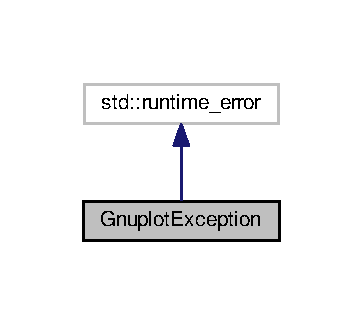
\includegraphics[width=174pt]{class_gnuplot_exception__inherit__graph}
\end{center}
\end{figure}


Collaboration diagram for Gnuplot\+Exception\+:
\nopagebreak
\begin{figure}[H]
\begin{center}
\leavevmode
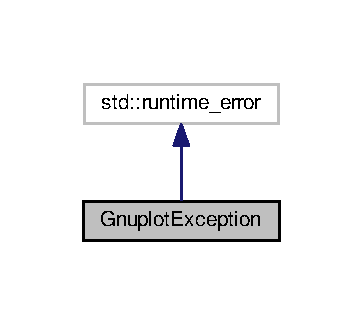
\includegraphics[width=174pt]{class_gnuplot_exception__coll__graph}
\end{center}
\end{figure}
\subsection*{Public Member Functions}
\begin{DoxyCompactItemize}
\item 
\mbox{\Hypertarget{class_gnuplot_exception_a8b324a9ef4d3f75079d41ecd61c62d44}\label{class_gnuplot_exception_a8b324a9ef4d3f75079d41ecd61c62d44}} 
{\bfseries Gnuplot\+Exception} (const std\+::string \&msg)
\end{DoxyCompactItemize}


\subsection{Detailed Description}
A C++ interface to gnuplot. 

The interface uses pipes and so won\textquotesingle{}t run on a system that doesn\textquotesingle{}t have P\+O\+S\+IX pipe support Tested on Windows (Min\+GW and Visual C++) and Linux (G\+CC)

Version history\+: 0. C interface by N. Devillard (27/01/03)
\begin{DoxyEnumerate}
\item C++ interface\+: direct translation from the C interface by Rajarshi Guha (07/03/03)
\item corrections for Win32 compatibility by V. Chyzhdzenka (20/05/03)
\item some member functions added, corrections for Win32 and Linux compatibility by M. Burgis (10/03/08)
\item Move function definition into gnuplot\+\_\+i.\+cpp by X. B\+R\+O\+Q\+U\+E\+RE (25/10/11)
\end{DoxyEnumerate}

Requirements\+:
\begin{DoxyItemize}
\item gnuplot has to be installed (\href{http://www.gnuplot.info/download.html}{\tt http\+://www.\+gnuplot.\+info/download.\+html})
\item for Windows\+: set Path-\/\+Variable for \hyperlink{class_gnuplot}{Gnuplot} path (e.\+g. C\+:/program files/gnuplot/bin) or set \hyperlink{class_gnuplot}{Gnuplot} path with\+: \hyperlink{class_gnuplot_a67cae885c26ced821e335d98986f1967}{Gnuplot\+::set\+\_\+\+G\+N\+U\+Plot\+Path(const std\+::string \&path)}; 
\end{DoxyItemize}

The documentation for this class was generated from the following file\+:\begin{DoxyCompactItemize}
\item 
includes/gnuplot\+\_\+i.\+hpp\end{DoxyCompactItemize}

\hypertarget{class_i_m_a_dual}{}\section{I\+M\+A\+Dual$<$ T $>$ Class Template Reference}
\label{class_i_m_a_dual}\index{I\+M\+A\+Dual$<$ T $>$@{I\+M\+A\+Dual$<$ T $>$}}


Inheritance diagram for I\+M\+A\+Dual$<$ T $>$\+:\nopagebreak
\begin{figure}[H]
\begin{center}
\leavevmode
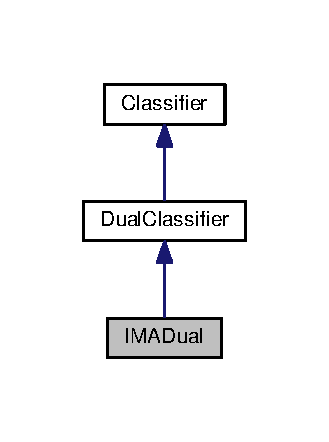
\includegraphics[width=158pt]{class_i_m_a_dual__inherit__graph}
\end{center}
\end{figure}


Collaboration diagram for I\+M\+A\+Dual$<$ T $>$\+:
\nopagebreak
\begin{figure}[H]
\begin{center}
\leavevmode
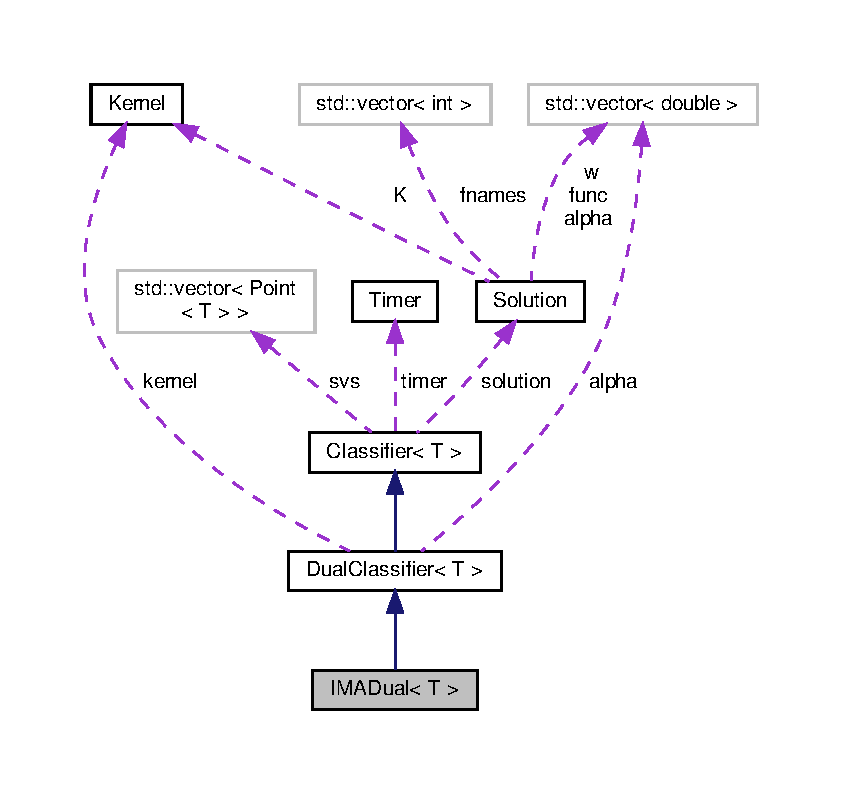
\includegraphics[width=350pt]{class_i_m_a_dual__coll__graph}
\end{center}
\end{figure}
\subsection*{Public Member Functions}
\begin{DoxyCompactItemize}
\item 
\mbox{\Hypertarget{class_i_m_a_dual_a22a5cf72fe88fd8bb846cf1b5758d61c}\label{class_i_m_a_dual_a22a5cf72fe88fd8bb846cf1b5758d61c}} 
{\bfseries I\+M\+A\+Dual} (std\+::shared\+\_\+ptr$<$ \hyperlink{class_data}{Data}$<$ T $>$ $>$ \hyperlink{class_classifier_a0000b47a2e0784ada4c52d7046c4adb8}{samples}=nullptr, \hyperlink{class_kernel}{Kernel} $\ast$k=nullptr, double \hyperlink{class_classifier_a7b1c4ef87631bd9e46682e5bc4315111}{rate}=1, \hyperlink{class_solution}{Solution} $\ast$initial\+\_\+solution=nullptr)
\item 
bool \hyperlink{class_i_m_a_dual_aff820af6454ceeef4d23af48476d7218}{train} () override
\begin{DoxyCompactList}\small\item\em Function that execute the training phase of a classification algorithm. \end{DoxyCompactList}\item 
double \hyperlink{class_i_m_a_dual_af67dfc75554d055cfdf761ee940243d7}{evaluate} (\hyperlink{class_point}{Point}$<$ T $>$ p) override
\begin{DoxyCompactList}\small\item\em Returns the class of a feature point based on the trained classifier. \end{DoxyCompactList}\end{DoxyCompactItemize}
\subsection*{Additional Inherited Members}


\subsection{Member Function Documentation}
\mbox{\Hypertarget{class_i_m_a_dual_af67dfc75554d055cfdf761ee940243d7}\label{class_i_m_a_dual_af67dfc75554d055cfdf761ee940243d7}} 
\index{I\+M\+A\+Dual@{I\+M\+A\+Dual}!evaluate@{evaluate}}
\index{evaluate@{evaluate}!I\+M\+A\+Dual@{I\+M\+A\+Dual}}
\subsubsection{\texorpdfstring{evaluate()}{evaluate()}}
{\footnotesize\ttfamily template$<$typename T $>$ \\
double \hyperlink{class_i_m_a_dual}{I\+M\+A\+Dual}$<$ T $>$\+::evaluate (\begin{DoxyParamCaption}\item[{\hyperlink{class_point}{Point}$<$ T $>$}]{p }\end{DoxyParamCaption})\hspace{0.3cm}{\ttfamily [override]}, {\ttfamily [virtual]}}



Returns the class of a feature point based on the trained classifier. 


\begin{DoxyParams}{Parameters}
{\em Point$<$} & T $>$ x (???) Features point to be evaluated. \\
\hline
\end{DoxyParams}
\begin{DoxyReturn}{Returns}
int 
\end{DoxyReturn}


Implements \hyperlink{class_classifier_ab3b9544a8d9c3cbde8d5865c7e9be0fb}{Classifier$<$ T $>$}.

\mbox{\Hypertarget{class_i_m_a_dual_aff820af6454ceeef4d23af48476d7218}\label{class_i_m_a_dual_aff820af6454ceeef4d23af48476d7218}} 
\index{I\+M\+A\+Dual@{I\+M\+A\+Dual}!train@{train}}
\index{train@{train}!I\+M\+A\+Dual@{I\+M\+A\+Dual}}
\subsubsection{\texorpdfstring{train()}{train()}}
{\footnotesize\ttfamily template$<$typename T $>$ \\
bool \hyperlink{class_i_m_a_dual}{I\+M\+A\+Dual}$<$ T $>$\+::train (\begin{DoxyParamCaption}{ }\end{DoxyParamCaption})\hspace{0.3cm}{\ttfamily [override]}, {\ttfamily [virtual]}}



Function that execute the training phase of a classification algorithm. 

\begin{DoxyReturn}{Returns}
void 
\end{DoxyReturn}


Implements \hyperlink{class_classifier_a120849bfdfa3ba7a0388b32b2d76bf4f}{Classifier$<$ T $>$}.



The documentation for this class was generated from the following files\+:\begin{DoxyCompactItemize}
\item 
includes/I\+M\+A.\+hpp\item 
src/I\+M\+A.\+cpp\end{DoxyCompactItemize}

\hypertarget{class_i_m_ap}{}\section{I\+M\+Ap$<$ T $>$ Class Template Reference}
\label{class_i_m_ap}\index{I\+M\+Ap$<$ T $>$@{I\+M\+Ap$<$ T $>$}}


Wrapper for the implementation of the Incremental Margin Algorithm primal.  




{\ttfamily \#include $<$I\+M\+A.\+hpp$>$}



Inheritance diagram for I\+M\+Ap$<$ T $>$\+:
\nopagebreak
\begin{figure}[H]
\begin{center}
\leavevmode
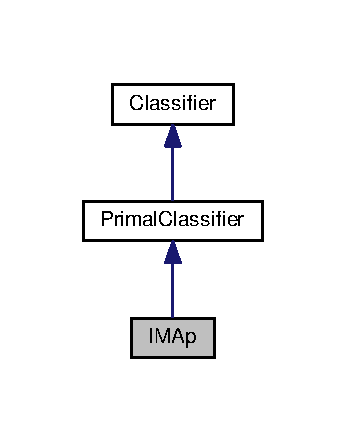
\includegraphics[width=197pt]{class_i_m_ap__inherit__graph}
\end{center}
\end{figure}


Collaboration diagram for I\+M\+Ap$<$ T $>$\+:
\nopagebreak
\begin{figure}[H]
\begin{center}
\leavevmode
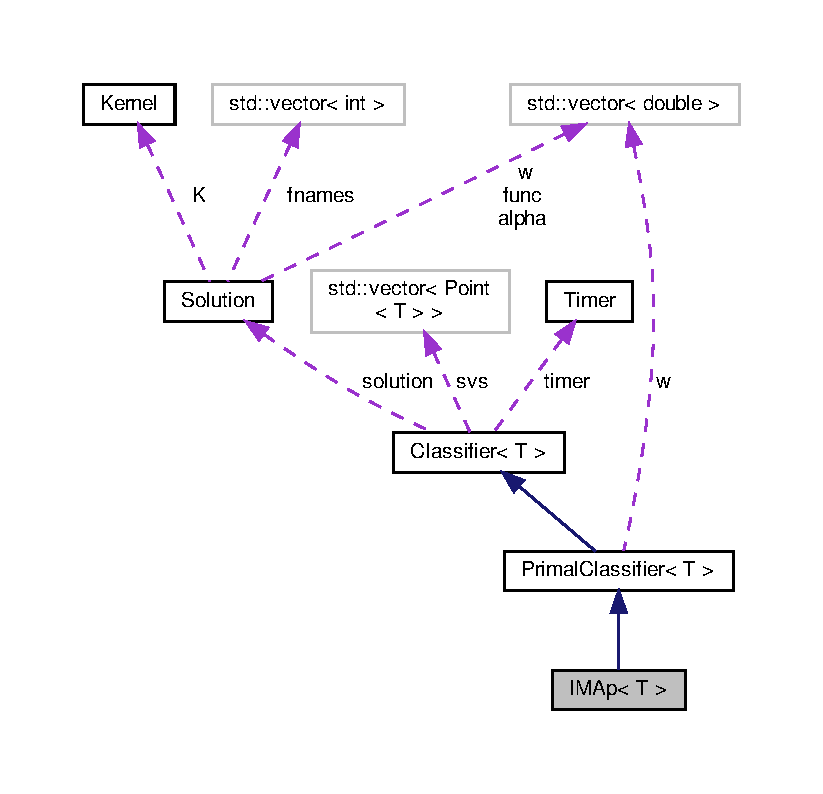
\includegraphics[width=350pt]{class_i_m_ap__coll__graph}
\end{center}
\end{figure}
\subsection*{Public Member Functions}
\begin{DoxyCompactItemize}
\item 
{\bfseries I\+M\+Ap} (std\+::shared\+\_\+ptr$<$ \hyperlink{class_data}{Data}$<$ T $>$ $>$ \hyperlink{class_classifier_a0000b47a2e0784ada4c52d7046c4adb8}{samples}=nullptr, double margin=0.\+0, \hyperlink{class_solution}{Solution} $\ast$initial\+\_\+solution=nullptr)\hypertarget{class_i_m_ap_a54d31e0bcbb062d224a40fdb3a9fcdcd}{}\label{class_i_m_ap_a54d31e0bcbb062d224a40fdb3a9fcdcd}

\item 
bool \hyperlink{class_i_m_ap_aa8bf6b0d21a76d388fe81ee516b627e4}{train} () override
\begin{DoxyCompactList}\small\item\em Function that execute the training phase of a classification algorithm. \end{DoxyCompactList}\item 
double \hyperlink{class_i_m_ap_a41b0739cdc486e3f21e7927f1ad429a8}{evaluate} (\hyperlink{class_point}{Point}$<$ T $>$ p) override
\begin{DoxyCompactList}\small\item\em Returns the class of a feature point based on the trained classifier. \end{DoxyCompactList}\item 
std\+::vector$<$ int $>$ \hyperlink{class_i_m_ap_a87adda768f1c48c0e4fcdf66f3145ae9}{get\+Support\+Vectors} ()
\begin{DoxyCompactList}\small\item\em Get the indexes of the support vectors. \end{DoxyCompactList}\end{DoxyCompactItemize}
\subsection*{Additional Inherited Members}


\subsection{Detailed Description}
\subsubsection*{template$<$typename T$>$\\*
class I\+M\+Ap$<$ T $>$}

Wrapper for the implementation of the Incremental Margin Algorithm primal. 

\subsection{Member Function Documentation}
\index{I\+M\+Ap@{I\+M\+Ap}!evaluate@{evaluate}}
\index{evaluate@{evaluate}!I\+M\+Ap@{I\+M\+Ap}}
\subsubsection[{\texorpdfstring{evaluate(\+Point$<$ T $>$ p) override}{evaluate(Point< T > p) override}}]{\setlength{\rightskip}{0pt plus 5cm}template$<$typename T $>$ double {\bf I\+M\+Ap}$<$ T $>$\+::evaluate (
\begin{DoxyParamCaption}
\item[{{\bf Point}$<$ T $>$}]{p}
\end{DoxyParamCaption}
)\hspace{0.3cm}{\ttfamily [override]}, {\ttfamily [virtual]}}\hypertarget{class_i_m_ap_a41b0739cdc486e3f21e7927f1ad429a8}{}\label{class_i_m_ap_a41b0739cdc486e3f21e7927f1ad429a8}


Returns the class of a feature point based on the trained classifier. 


\begin{DoxyParams}{Parameters}
{\em Point$<$} & T $>$ x (???) Features point to be evaluated. \\
\hline
\end{DoxyParams}
\begin{DoxyReturn}{Returns}
int 
\end{DoxyReturn}


Implements \hyperlink{class_classifier_ab3b9544a8d9c3cbde8d5865c7e9be0fb}{Classifier$<$ T $>$}.

\index{I\+M\+Ap@{I\+M\+Ap}!get\+Support\+Vectors@{get\+Support\+Vectors}}
\index{get\+Support\+Vectors@{get\+Support\+Vectors}!I\+M\+Ap@{I\+M\+Ap}}
\subsubsection[{\texorpdfstring{get\+Support\+Vectors()}{getSupportVectors()}}]{\setlength{\rightskip}{0pt plus 5cm}template$<$typename T $>$ std\+::vector$<$int$>$ {\bf I\+M\+Ap}$<$ T $>$\+::get\+Support\+Vectors (
\begin{DoxyParamCaption}
{}
\end{DoxyParamCaption}
)\hspace{0.3cm}{\ttfamily [inline]}}\hypertarget{class_i_m_ap_a87adda768f1c48c0e4fcdf66f3145ae9}{}\label{class_i_m_ap_a87adda768f1c48c0e4fcdf66f3145ae9}


Get the indexes of the support vectors. 

\begin{DoxyReturn}{Returns}
std\+::vector$<$int$>$ 
\end{DoxyReturn}
\index{I\+M\+Ap@{I\+M\+Ap}!train@{train}}
\index{train@{train}!I\+M\+Ap@{I\+M\+Ap}}
\subsubsection[{\texorpdfstring{train() override}{train() override}}]{\setlength{\rightskip}{0pt plus 5cm}template$<$typename T $>$ bool {\bf I\+M\+Ap}$<$ T $>$\+::train (
\begin{DoxyParamCaption}
{}
\end{DoxyParamCaption}
)\hspace{0.3cm}{\ttfamily [override]}, {\ttfamily [virtual]}}\hypertarget{class_i_m_ap_aa8bf6b0d21a76d388fe81ee516b627e4}{}\label{class_i_m_ap_aa8bf6b0d21a76d388fe81ee516b627e4}


Function that execute the training phase of a classification algorithm. 

\begin{DoxyReturn}{Returns}
void 
\end{DoxyReturn}


Implements \hyperlink{class_classifier_a120849bfdfa3ba7a0388b32b2d76bf4f}{Classifier$<$ T $>$}.



The documentation for this class was generated from the following files\+:\begin{DoxyCompactItemize}
\item 
includes/\hyperlink{_i_m_a_8hpp}{I\+M\+A.\+hpp}\item 
src/I\+M\+A.\+cpp\end{DoxyCompactItemize}

\hypertarget{class_i_m_ap_fixed_margin}{}\section{I\+M\+Ap\+Fixed\+Margin$<$ T $>$ Class Template Reference}
\label{class_i_m_ap_fixed_margin}\index{I\+M\+Ap\+Fixed\+Margin$<$ T $>$@{I\+M\+Ap\+Fixed\+Margin$<$ T $>$}}


Wrapper for the implementation of the Incremental Margin Algorithm primal with fixed margin.  




{\ttfamily \#include $<$I\+M\+A.\+hpp$>$}



Inheritance diagram for I\+M\+Ap\+Fixed\+Margin$<$ T $>$\+:
\nopagebreak
\begin{figure}[H]
\begin{center}
\leavevmode
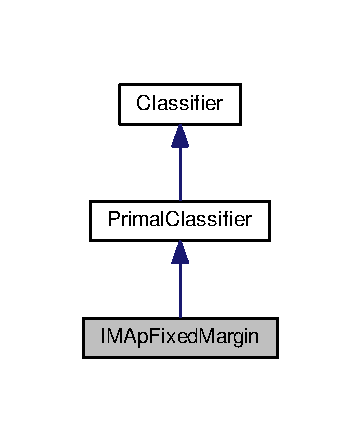
\includegraphics[width=204pt]{class_i_m_ap_fixed_margin__inherit__graph}
\end{center}
\end{figure}


Collaboration diagram for I\+M\+Ap\+Fixed\+Margin$<$ T $>$\+:
\nopagebreak
\begin{figure}[H]
\begin{center}
\leavevmode
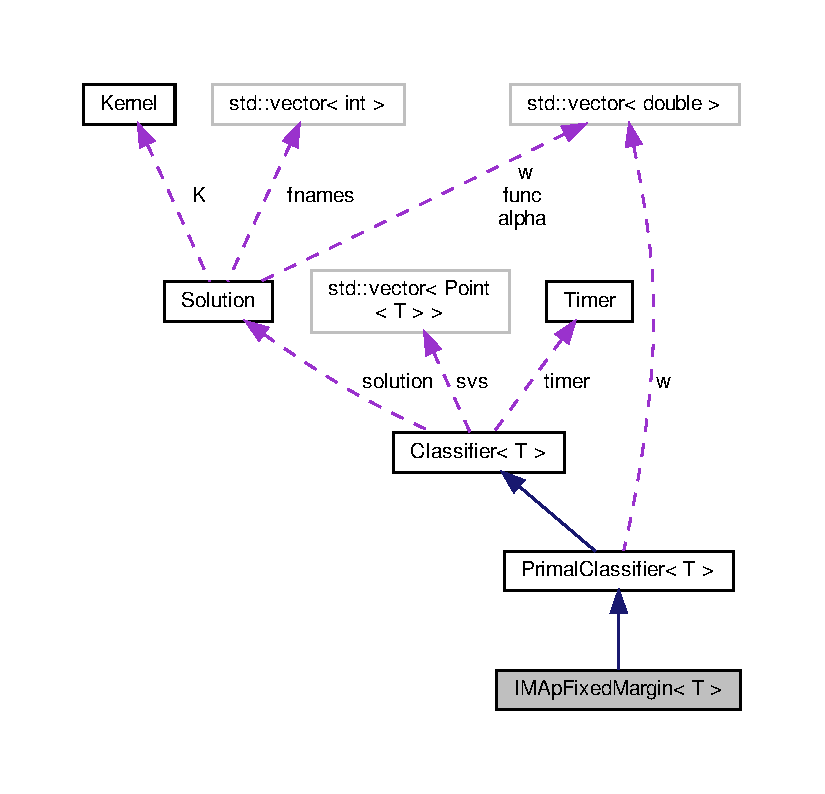
\includegraphics[width=350pt]{class_i_m_ap_fixed_margin__coll__graph}
\end{center}
\end{figure}
\subsection*{Public Member Functions}
\begin{DoxyCompactItemize}
\item 
{\bfseries I\+M\+Ap\+Fixed\+Margin} (std\+::shared\+\_\+ptr$<$ \hyperlink{class_data}{Data}$<$ T $>$ $>$ \hyperlink{class_classifier_a0000b47a2e0784ada4c52d7046c4adb8}{samples}=nullptr, double gamma=0, \hyperlink{class_solution}{Solution} $\ast$initial\+\_\+solution=nullptr)\hypertarget{class_i_m_ap_fixed_margin_a90724da378b06629c891dea9fa49e379}{}\label{class_i_m_ap_fixed_margin_a90724da378b06629c891dea9fa49e379}

\item 
bool \hyperlink{class_i_m_ap_fixed_margin_a4d99742be5fe5a21b8ae6f99547a98c8}{train} () override
\begin{DoxyCompactList}\small\item\em Function that execute the training phase of a classification algorithm. \end{DoxyCompactList}\item 
double \hyperlink{class_i_m_ap_fixed_margin_a909eb58c78c20780494598b478f8846f}{evaluate} (\hyperlink{class_point}{Point}$<$ T $>$ p) override
\begin{DoxyCompactList}\small\item\em Returns the class of a feature point based on the trained classifier. \end{DoxyCompactList}\item 
int $\ast$ {\bfseries get\+Flag\+Not1a\+Dim} ()\hypertarget{class_i_m_ap_fixed_margin_ac928b3c55da2171adce3231223f85d42}{}\label{class_i_m_ap_fixed_margin_ac928b3c55da2171adce3231223f85d42}

\item 
unsigned long $\ast$ {\bfseries gett\+Max} ()\hypertarget{class_i_m_ap_fixed_margin_a90bd97bde25c511399400a85a5f786e2}{}\label{class_i_m_ap_fixed_margin_a90bd97bde25c511399400a85a5f786e2}

\end{DoxyCompactItemize}
\subsection*{Additional Inherited Members}


\subsection{Detailed Description}
\subsubsection*{template$<$typename T$>$\\*
class I\+M\+Ap\+Fixed\+Margin$<$ T $>$}

Wrapper for the implementation of the Incremental Margin Algorithm primal with fixed margin. 

\subsection{Member Function Documentation}
\index{I\+M\+Ap\+Fixed\+Margin@{I\+M\+Ap\+Fixed\+Margin}!evaluate@{evaluate}}
\index{evaluate@{evaluate}!I\+M\+Ap\+Fixed\+Margin@{I\+M\+Ap\+Fixed\+Margin}}
\subsubsection[{\texorpdfstring{evaluate(\+Point$<$ T $>$ p) override}{evaluate(Point< T > p) override}}]{\setlength{\rightskip}{0pt plus 5cm}template$<$typename T $>$ double {\bf I\+M\+Ap\+Fixed\+Margin}$<$ T $>$\+::evaluate (
\begin{DoxyParamCaption}
\item[{{\bf Point}$<$ T $>$}]{p}
\end{DoxyParamCaption}
)\hspace{0.3cm}{\ttfamily [override]}, {\ttfamily [virtual]}}\hypertarget{class_i_m_ap_fixed_margin_a909eb58c78c20780494598b478f8846f}{}\label{class_i_m_ap_fixed_margin_a909eb58c78c20780494598b478f8846f}


Returns the class of a feature point based on the trained classifier. 


\begin{DoxyParams}{Parameters}
{\em Point$<$} & T $>$ x (???) Features point to be evaluated. \\
\hline
\end{DoxyParams}
\begin{DoxyReturn}{Returns}
int 
\end{DoxyReturn}


Implements \hyperlink{class_classifier_ab3b9544a8d9c3cbde8d5865c7e9be0fb}{Classifier$<$ T $>$}.

\index{I\+M\+Ap\+Fixed\+Margin@{I\+M\+Ap\+Fixed\+Margin}!train@{train}}
\index{train@{train}!I\+M\+Ap\+Fixed\+Margin@{I\+M\+Ap\+Fixed\+Margin}}
\subsubsection[{\texorpdfstring{train() override}{train() override}}]{\setlength{\rightskip}{0pt plus 5cm}template$<$typename T $>$ bool {\bf I\+M\+Ap\+Fixed\+Margin}$<$ T $>$\+::train (
\begin{DoxyParamCaption}
{}
\end{DoxyParamCaption}
)\hspace{0.3cm}{\ttfamily [override]}, {\ttfamily [virtual]}}\hypertarget{class_i_m_ap_fixed_margin_a4d99742be5fe5a21b8ae6f99547a98c8}{}\label{class_i_m_ap_fixed_margin_a4d99742be5fe5a21b8ae6f99547a98c8}


Function that execute the training phase of a classification algorithm. 

\begin{DoxyReturn}{Returns}
void 
\end{DoxyReturn}


Implements \hyperlink{class_classifier_a120849bfdfa3ba7a0388b32b2d76bf4f}{Classifier$<$ T $>$}.



The documentation for this class was generated from the following files\+:\begin{DoxyCompactItemize}
\item 
includes/\hyperlink{_i_m_a_8hpp}{I\+M\+A.\+hpp}\item 
src/I\+M\+A.\+cpp\end{DoxyCompactItemize}

\hypertarget{class_kernel}{}\section{Kernel Class Reference}
\label{class_kernel}\index{Kernel@{Kernel}}


Class for the kernel computations.  




{\ttfamily \#include $<$Kernel.\+hpp$>$}

\subsection*{Public Member Functions}
\begin{DoxyCompactItemize}
\item 
\mbox{\Hypertarget{class_kernel_ae60e072c58cdc16842a239bdd0761590}\label{class_kernel_ae60e072c58cdc16842a239bdd0761590}} 
\hyperlink{class_kernel_ae60e072c58cdc16842a239bdd0761590}{Kernel} (int type=0, double param=0)
\begin{DoxyCompactList}\small\item\em Class constructor. \end{DoxyCompactList}\item 
\hyperlink{class_kernel_adf23c1567adb8ddb5757931587320871}{Kernel} (d\+Matrix kernel\+\_\+matrix)
\begin{DoxyCompactList}\small\item\em Class constructor. \end{DoxyCompactList}\item 
void \hyperlink{class_kernel_ad01e209470accf44ea240078f39fb127}{set\+Type} (int type)
\begin{DoxyCompactList}\small\item\em set\+Type Set the kernel type used in the kernel computations. \end{DoxyCompactList}\item 
void \hyperlink{class_kernel_a4fe711ebdbc168be1733fbb8aea6cf92}{set\+Param} (int param)
\begin{DoxyCompactList}\small\item\em set\+Param Set the kernel parameter used in the kernel computations. \end{DoxyCompactList}\item 
int \hyperlink{class_kernel_a5a2cb0fce0eda6c67a2325f6c8958da8}{get\+Type} ()
\begin{DoxyCompactList}\small\item\em get\+Type Returns the kernel type used in the kernel computations. \end{DoxyCompactList}\item 
double \hyperlink{class_kernel_a838e2cc5018fa702e59c52a3bf8ef813}{get\+Param} ()
\begin{DoxyCompactList}\small\item\em get\+Param Returns the kernel parameter used in the kernel computations. \end{DoxyCompactList}\item 
void \hyperlink{class_kernel_a3801cee0d86f25f1500d202f43a84b65}{set\+Kernel\+Matrix} (d\+Matrix K)
\begin{DoxyCompactList}\small\item\em set\+Kernel\+Matrix Set a pre computed kernel matrix. \end{DoxyCompactList}\item 
d\+Matrix \hyperlink{class_kernel_a5e398c63fee5f0e30b6dfb735c75e41a}{get\+Kernel\+Matrix} ()
\begin{DoxyCompactList}\small\item\em get\+Kernel\+Matrix Get the kernel matrix. \end{DoxyCompactList}\item 
void \hyperlink{class_kernel_a5dfd3a6b535745eadd9e17dc086d87c6}{compute} (\hyperlink{class_data}{Data} samples)
\begin{DoxyCompactList}\small\item\em compute Compute the kernel matrix with the given type and parameter. \end{DoxyCompactList}\item 
double \hyperlink{class_kernel_aa07703cd76124769325d942582b16b5f}{function} (std\+::shared\+\_\+ptr$<$ \hyperlink{class_point}{Point} $>$ one, std\+::shared\+\_\+ptr$<$ \hyperlink{class_point}{Point} $>$ two, int dim)
\begin{DoxyCompactList}\small\item\em function Compute the kernel function between two points. \end{DoxyCompactList}\item 
double \hyperlink{class_kernel_a1f548d2e5477ae0ee3dd3bc7f23e6920}{norm} (\hyperlink{class_data}{Data} data)
\begin{DoxyCompactList}\small\item\em norm Computes norm in dual variables. \end{DoxyCompactList}\end{DoxyCompactItemize}


\subsection{Detailed Description}
Class for the kernel computations. 

\subsection{Constructor \& Destructor Documentation}
\mbox{\Hypertarget{class_kernel_adf23c1567adb8ddb5757931587320871}\label{class_kernel_adf23c1567adb8ddb5757931587320871}} 
\index{Kernel@{Kernel}!Kernel@{Kernel}}
\index{Kernel@{Kernel}!Kernel@{Kernel}}
\subsubsection{\texorpdfstring{Kernel()}{Kernel()}}
{\footnotesize\ttfamily Kernel\+::\+Kernel (\begin{DoxyParamCaption}\item[{d\+Matrix}]{kernel\+\_\+matrix }\end{DoxyParamCaption})}



Class constructor. 


\begin{DoxyParams}{Parameters}
{\em K} & \hyperlink{class_kernel}{Kernel} matrix to be set in initialization. \\
\hline
\end{DoxyParams}


\subsection{Member Function Documentation}
\mbox{\Hypertarget{class_kernel_a5dfd3a6b535745eadd9e17dc086d87c6}\label{class_kernel_a5dfd3a6b535745eadd9e17dc086d87c6}} 
\index{Kernel@{Kernel}!compute@{compute}}
\index{compute@{compute}!Kernel@{Kernel}}
\subsubsection{\texorpdfstring{compute()}{compute()}}
{\footnotesize\ttfamily void Kernel\+::compute (\begin{DoxyParamCaption}\item[{\hyperlink{class_data}{Data}}]{samples }\end{DoxyParamCaption})}



compute Compute the kernel matrix with the given type and parameter. 


\begin{DoxyParams}{Parameters}
{\em samples} & \hyperlink{class_data}{Data} used to compute the kernel matrix. \\
\hline
\end{DoxyParams}
\mbox{\Hypertarget{class_kernel_aa07703cd76124769325d942582b16b5f}\label{class_kernel_aa07703cd76124769325d942582b16b5f}} 
\index{Kernel@{Kernel}!function@{function}}
\index{function@{function}!Kernel@{Kernel}}
\subsubsection{\texorpdfstring{function()}{function()}}
{\footnotesize\ttfamily double Kernel\+::function (\begin{DoxyParamCaption}\item[{std\+::shared\+\_\+ptr$<$ \hyperlink{class_point}{Point} $>$}]{one,  }\item[{std\+::shared\+\_\+ptr$<$ \hyperlink{class_point}{Point} $>$}]{two,  }\item[{int}]{dim }\end{DoxyParamCaption})}



function Compute the kernel function between two points. 


\begin{DoxyParams}{Parameters}
{\em one} & first point. \\
\hline
{\em two} & second point. \\
\hline
{\em dim} & Dimension of the points. \\
\hline
\end{DoxyParams}
\begin{DoxyReturn}{Returns}
double 
\end{DoxyReturn}
\mbox{\Hypertarget{class_kernel_a5e398c63fee5f0e30b6dfb735c75e41a}\label{class_kernel_a5e398c63fee5f0e30b6dfb735c75e41a}} 
\index{Kernel@{Kernel}!get\+Kernel\+Matrix@{get\+Kernel\+Matrix}}
\index{get\+Kernel\+Matrix@{get\+Kernel\+Matrix}!Kernel@{Kernel}}
\subsubsection{\texorpdfstring{get\+Kernel\+Matrix()}{getKernelMatrix()}}
{\footnotesize\ttfamily d\+Matrix Kernel\+::get\+Kernel\+Matrix (\begin{DoxyParamCaption}{ }\end{DoxyParamCaption})}



get\+Kernel\+Matrix Get the kernel matrix. 

\begin{DoxyReturn}{Returns}
std\+::vector$<$std\+::vector$<$double$>$ $>$ 
\end{DoxyReturn}
\mbox{\Hypertarget{class_kernel_a838e2cc5018fa702e59c52a3bf8ef813}\label{class_kernel_a838e2cc5018fa702e59c52a3bf8ef813}} 
\index{Kernel@{Kernel}!get\+Param@{get\+Param}}
\index{get\+Param@{get\+Param}!Kernel@{Kernel}}
\subsubsection{\texorpdfstring{get\+Param()}{getParam()}}
{\footnotesize\ttfamily double Kernel\+::get\+Param (\begin{DoxyParamCaption}{ }\end{DoxyParamCaption})}



get\+Param Returns the kernel parameter used in the kernel computations. 

\begin{DoxyReturn}{Returns}
double 
\end{DoxyReturn}
\mbox{\Hypertarget{class_kernel_a5a2cb0fce0eda6c67a2325f6c8958da8}\label{class_kernel_a5a2cb0fce0eda6c67a2325f6c8958da8}} 
\index{Kernel@{Kernel}!get\+Type@{get\+Type}}
\index{get\+Type@{get\+Type}!Kernel@{Kernel}}
\subsubsection{\texorpdfstring{get\+Type()}{getType()}}
{\footnotesize\ttfamily int Kernel\+::get\+Type (\begin{DoxyParamCaption}{ }\end{DoxyParamCaption})}



get\+Type Returns the kernel type used in the kernel computations. 

\begin{DoxyReturn}{Returns}
int. 
\end{DoxyReturn}
\mbox{\Hypertarget{class_kernel_a1f548d2e5477ae0ee3dd3bc7f23e6920}\label{class_kernel_a1f548d2e5477ae0ee3dd3bc7f23e6920}} 
\index{Kernel@{Kernel}!norm@{norm}}
\index{norm@{norm}!Kernel@{Kernel}}
\subsubsection{\texorpdfstring{norm()}{norm()}}
{\footnotesize\ttfamily double Kernel\+::norm (\begin{DoxyParamCaption}\item[{\hyperlink{class_data}{Data}}]{data }\end{DoxyParamCaption})}



norm Computes norm in dual variables. 


\begin{DoxyParams}{Parameters}
{\em data} & Dataset to compute norm. \\
\hline
\end{DoxyParams}
\begin{DoxyReturn}{Returns}
double 
\end{DoxyReturn}
\mbox{\Hypertarget{class_kernel_a3801cee0d86f25f1500d202f43a84b65}\label{class_kernel_a3801cee0d86f25f1500d202f43a84b65}} 
\index{Kernel@{Kernel}!set\+Kernel\+Matrix@{set\+Kernel\+Matrix}}
\index{set\+Kernel\+Matrix@{set\+Kernel\+Matrix}!Kernel@{Kernel}}
\subsubsection{\texorpdfstring{set\+Kernel\+Matrix()}{setKernelMatrix()}}
{\footnotesize\ttfamily void Kernel\+::set\+Kernel\+Matrix (\begin{DoxyParamCaption}\item[{d\+Matrix}]{K }\end{DoxyParamCaption})}



set\+Kernel\+Matrix Set a pre computed kernel matrix. 


\begin{DoxyParams}{Parameters}
{\em K} & \hyperlink{class_kernel}{Kernel} matrix to be set. \\
\hline
\end{DoxyParams}
\mbox{\Hypertarget{class_kernel_a4fe711ebdbc168be1733fbb8aea6cf92}\label{class_kernel_a4fe711ebdbc168be1733fbb8aea6cf92}} 
\index{Kernel@{Kernel}!set\+Param@{set\+Param}}
\index{set\+Param@{set\+Param}!Kernel@{Kernel}}
\subsubsection{\texorpdfstring{set\+Param()}{setParam()}}
{\footnotesize\ttfamily void Kernel\+::set\+Param (\begin{DoxyParamCaption}\item[{int}]{param }\end{DoxyParamCaption})}



set\+Param Set the kernel parameter used in the kernel computations. 


\begin{DoxyParams}{Parameters}
{\em param} & parameter to be set. \\
\hline
\end{DoxyParams}
\mbox{\Hypertarget{class_kernel_ad01e209470accf44ea240078f39fb127}\label{class_kernel_ad01e209470accf44ea240078f39fb127}} 
\index{Kernel@{Kernel}!set\+Type@{set\+Type}}
\index{set\+Type@{set\+Type}!Kernel@{Kernel}}
\subsubsection{\texorpdfstring{set\+Type()}{setType()}}
{\footnotesize\ttfamily void Kernel\+::set\+Type (\begin{DoxyParamCaption}\item[{int}]{type }\end{DoxyParamCaption})}



set\+Type Set the kernel type used in the kernel computations. 


\begin{DoxyParams}{Parameters}
{\em type} & \hyperlink{class_kernel}{Kernel} type. \\
\hline
\end{DoxyParams}


The documentation for this class was generated from the following files\+:\begin{DoxyCompactItemize}
\item 
includes/Kernel.\+hpp\item 
src/Kernel.\+cpp\end{DoxyCompactItemize}

\hypertarget{class_perceptron_dual}{}\section{Perceptron\+Dual Class Reference}
\label{class_perceptron_dual}\index{Perceptron\+Dual@{Perceptron\+Dual}}


Wrapper for the implementation of the Perceptron dual algorithm.  




{\ttfamily \#include $<$Perceptron.\+hpp$>$}



Inheritance diagram for Perceptron\+Dual\+:\nopagebreak
\begin{figure}[H]
\begin{center}
\leavevmode
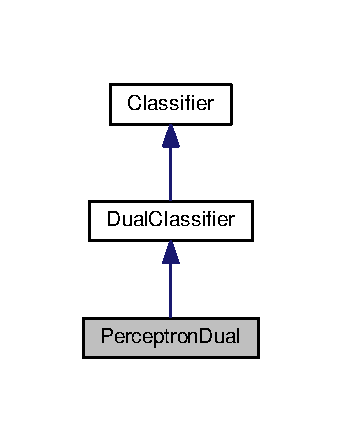
\includegraphics[width=164pt]{class_perceptron_dual__inherit__graph}
\end{center}
\end{figure}


Collaboration diagram for Perceptron\+Dual\+:\nopagebreak
\begin{figure}[H]
\begin{center}
\leavevmode
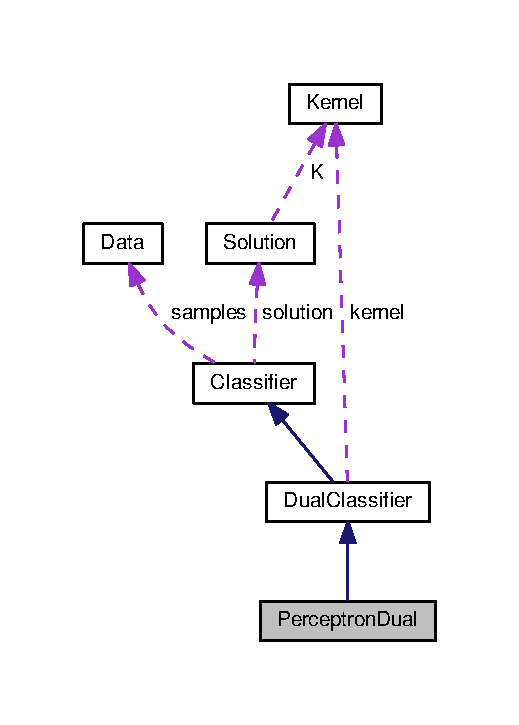
\includegraphics[width=242pt]{class_perceptron_dual__coll__graph}
\end{center}
\end{figure}
\subsection*{Public Member Functions}
\begin{DoxyCompactItemize}
\item 
\mbox{\Hypertarget{class_perceptron_dual_a7f1955774c5758e55232b88c2d8a048a}\label{class_perceptron_dual_a7f1955774c5758e55232b88c2d8a048a}} 
{\bfseries Perceptron\+Dual} (std\+::shared\+\_\+ptr$<$ \hyperlink{class_data}{Data} $>$ \hyperlink{class_classifier_aad6a4fcea8f44339d7a6302f530852ca}{samples}=nullptr, double \hyperlink{class_classifier_af9867e5919742de1303dd971a9a1c19a}{rate}=0.\+5, \hyperlink{class_kernel}{Kernel} $\ast$K=nullptr, \hyperlink{class_solution}{Solution} $\ast$initial\+\_\+solution=nullptr)
\item 
bool \hyperlink{class_perceptron_dual_a67acd9361cba43bbe2d682c4acd4ecaf}{train} () override
\begin{DoxyCompactList}\small\item\em Function that execute the training phase of a classification algorithm. \end{DoxyCompactList}\item 
double \hyperlink{class_perceptron_dual_af45407197f22fd513296f7a80e7683d9}{evaluate} (\hyperlink{class_point}{Point} p) override
\begin{DoxyCompactList}\small\item\em Returns the class of a feature point based on the trained classifier. \end{DoxyCompactList}\end{DoxyCompactItemize}
\subsection*{Additional Inherited Members}


\subsection{Detailed Description}
Wrapper for the implementation of the Perceptron dual algorithm. 

\subsection{Member Function Documentation}
\mbox{\Hypertarget{class_perceptron_dual_af45407197f22fd513296f7a80e7683d9}\label{class_perceptron_dual_af45407197f22fd513296f7a80e7683d9}} 
\index{Perceptron\+Dual@{Perceptron\+Dual}!evaluate@{evaluate}}
\index{evaluate@{evaluate}!Perceptron\+Dual@{Perceptron\+Dual}}
\subsubsection{\texorpdfstring{evaluate()}{evaluate()}}
{\footnotesize\ttfamily double Perceptron\+Dual\+::evaluate (\begin{DoxyParamCaption}\item[{\hyperlink{class_point}{Point}}]{p }\end{DoxyParamCaption})\hspace{0.3cm}{\ttfamily [override]}, {\ttfamily [virtual]}}



Returns the class of a feature point based on the trained classifier. 


\begin{DoxyParams}{Parameters}
{\em \hyperlink{class_point}{Point}} & x (???) Features point to be evaluated. \\
\hline
\end{DoxyParams}
\begin{DoxyReturn}{Returns}
int 
\end{DoxyReturn}


Implements \hyperlink{class_classifier_ae8e9554823b85ddc2dcad2955da811d9}{Classifier}.

\mbox{\Hypertarget{class_perceptron_dual_a67acd9361cba43bbe2d682c4acd4ecaf}\label{class_perceptron_dual_a67acd9361cba43bbe2d682c4acd4ecaf}} 
\index{Perceptron\+Dual@{Perceptron\+Dual}!train@{train}}
\index{train@{train}!Perceptron\+Dual@{Perceptron\+Dual}}
\subsubsection{\texorpdfstring{train()}{train()}}
{\footnotesize\ttfamily bool Perceptron\+Dual\+::train (\begin{DoxyParamCaption}{ }\end{DoxyParamCaption})\hspace{0.3cm}{\ttfamily [override]}, {\ttfamily [virtual]}}



Function that execute the training phase of a classification algorithm. 

\begin{DoxyReturn}{Returns}
void 
\end{DoxyReturn}


Implements \hyperlink{class_classifier_a2306a5de27555ab093593ac9642bc7d9}{Classifier}.



The documentation for this class was generated from the following files\+:\begin{DoxyCompactItemize}
\item 
includes/\hyperlink{_perceptron_8hpp}{Perceptron.\+hpp}\item 
src/Perceptron.\+cpp\end{DoxyCompactItemize}

\hypertarget{class_perceptron_fixed_margin_dual}{}\section{Perceptron\+Fixed\+Margin\+Dual Class Reference}
\label{class_perceptron_fixed_margin_dual}\index{Perceptron\+Fixed\+Margin\+Dual@{Perceptron\+Fixed\+Margin\+Dual}}


Wrapper for the implementation of the Perceptron dual with fixed margin algorithm.  




{\ttfamily \#include $<$Perceptron.\+hpp$>$}



Inheritance diagram for Perceptron\+Fixed\+Margin\+Dual\+:\nopagebreak
\begin{figure}[H]
\begin{center}
\leavevmode
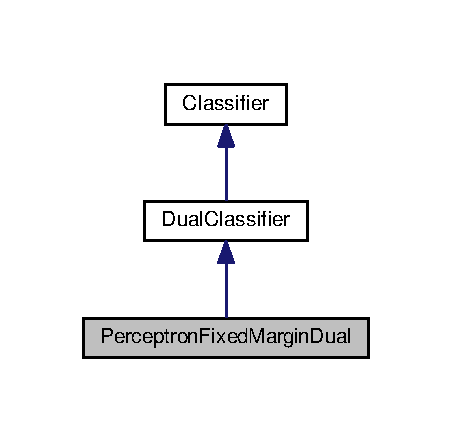
\includegraphics[width=217pt]{class_perceptron_fixed_margin_dual__inherit__graph}
\end{center}
\end{figure}


Collaboration diagram for Perceptron\+Fixed\+Margin\+Dual\+:\nopagebreak
\begin{figure}[H]
\begin{center}
\leavevmode
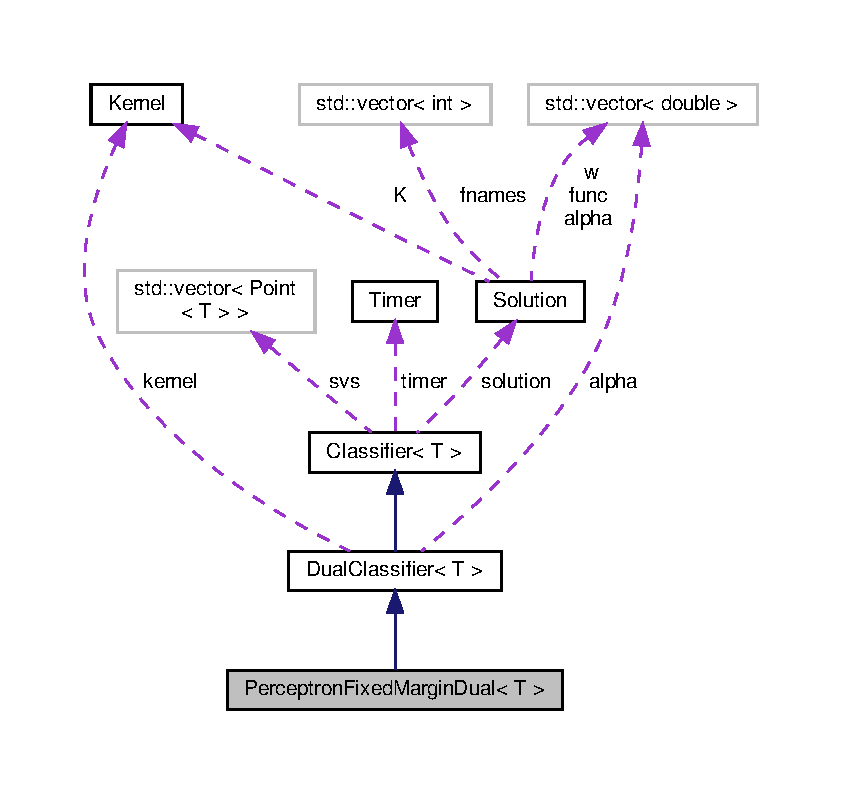
\includegraphics[width=276pt]{class_perceptron_fixed_margin_dual__coll__graph}
\end{center}
\end{figure}
\subsection*{Public Member Functions}
\begin{DoxyCompactItemize}
\item 
\mbox{\Hypertarget{class_perceptron_fixed_margin_dual_ac58bf42eac090bba4221e761fbe7fd0c}\label{class_perceptron_fixed_margin_dual_ac58bf42eac090bba4221e761fbe7fd0c}} 
{\bfseries Perceptron\+Fixed\+Margin\+Dual} (\hyperlink{class_data}{Data} $\ast$\hyperlink{class_classifier_a515c225d0da93df02ca79f9f87811d17}{samples}=N\+U\+LL, double gamma=1.\+0, double \hyperlink{class_classifier_af9867e5919742de1303dd971a9a1c19a}{rate}=0.\+5, \hyperlink{class_kernel}{Kernel} $\ast$K=N\+U\+LL, \hyperlink{class_solution}{Solution} $\ast$initial\+\_\+solution=N\+U\+LL)
\item 
bool \hyperlink{class_perceptron_fixed_margin_dual_aa095c90a3d04f70e1cf2e38e2afa769b}{train} ()
\begin{DoxyCompactList}\small\item\em Function that execute the training phase of a classification algorithm. \end{DoxyCompactList}\item 
double \hyperlink{class_perceptron_fixed_margin_dual_a1370fdbc95bf728f82a83f219be32d23}{evaluate} (\hyperlink{class_point}{Point} p)
\begin{DoxyCompactList}\small\item\em Returns the class of a feature point based on the trained classifier. \end{DoxyCompactList}\end{DoxyCompactItemize}
\subsection*{Additional Inherited Members}


\subsection{Detailed Description}
Wrapper for the implementation of the Perceptron dual with fixed margin algorithm. 

\subsection{Member Function Documentation}
\mbox{\Hypertarget{class_perceptron_fixed_margin_dual_a1370fdbc95bf728f82a83f219be32d23}\label{class_perceptron_fixed_margin_dual_a1370fdbc95bf728f82a83f219be32d23}} 
\index{Perceptron\+Fixed\+Margin\+Dual@{Perceptron\+Fixed\+Margin\+Dual}!evaluate@{evaluate}}
\index{evaluate@{evaluate}!Perceptron\+Fixed\+Margin\+Dual@{Perceptron\+Fixed\+Margin\+Dual}}
\subsubsection{\texorpdfstring{evaluate()}{evaluate()}}
{\footnotesize\ttfamily double Perceptron\+Fixed\+Margin\+Dual\+::evaluate (\begin{DoxyParamCaption}\item[{\hyperlink{class_point}{Point}}]{p }\end{DoxyParamCaption})\hspace{0.3cm}{\ttfamily [virtual]}}



Returns the class of a feature point based on the trained classifier. 


\begin{DoxyParams}{Parameters}
{\em \hyperlink{class_point}{Point}} & x (???) Features point to be evaluated. \\
\hline
\end{DoxyParams}
\begin{DoxyReturn}{Returns}
int 
\end{DoxyReturn}


Implements \hyperlink{class_classifier_ae8e9554823b85ddc2dcad2955da811d9}{Classifier}.

\mbox{\Hypertarget{class_perceptron_fixed_margin_dual_aa095c90a3d04f70e1cf2e38e2afa769b}\label{class_perceptron_fixed_margin_dual_aa095c90a3d04f70e1cf2e38e2afa769b}} 
\index{Perceptron\+Fixed\+Margin\+Dual@{Perceptron\+Fixed\+Margin\+Dual}!train@{train}}
\index{train@{train}!Perceptron\+Fixed\+Margin\+Dual@{Perceptron\+Fixed\+Margin\+Dual}}
\subsubsection{\texorpdfstring{train()}{train()}}
{\footnotesize\ttfamily bool Perceptron\+Fixed\+Margin\+Dual\+::train (\begin{DoxyParamCaption}{ }\end{DoxyParamCaption})\hspace{0.3cm}{\ttfamily [virtual]}}



Function that execute the training phase of a classification algorithm. 

\begin{DoxyReturn}{Returns}
void 
\end{DoxyReturn}


Implements \hyperlink{class_classifier_a2306a5de27555ab093593ac9642bc7d9}{Classifier}.



The documentation for this class was generated from the following files\+:\begin{DoxyCompactItemize}
\item 
includes/\hyperlink{_perceptron_8hpp}{Perceptron.\+hpp}\item 
src/Perceptron.\+cpp\end{DoxyCompactItemize}

\hypertarget{class_perceptron_fixed_margin_primal}{}\section{Perceptron\+Fixed\+Margin\+Primal Class Reference}
\label{class_perceptron_fixed_margin_primal}\index{Perceptron\+Fixed\+Margin\+Primal@{Perceptron\+Fixed\+Margin\+Primal}}


Wrapper for the implementation of the Perceptron primal with fixed margin algorithm.  




{\ttfamily \#include $<$Perceptron.\+hpp$>$}



Inheritance diagram for Perceptron\+Fixed\+Margin\+Primal\+:\nopagebreak
\begin{figure}[H]
\begin{center}
\leavevmode
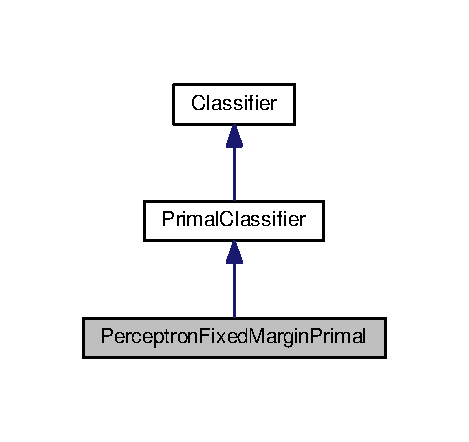
\includegraphics[width=225pt]{class_perceptron_fixed_margin_primal__inherit__graph}
\end{center}
\end{figure}


Collaboration diagram for Perceptron\+Fixed\+Margin\+Primal\+:\nopagebreak
\begin{figure}[H]
\begin{center}
\leavevmode
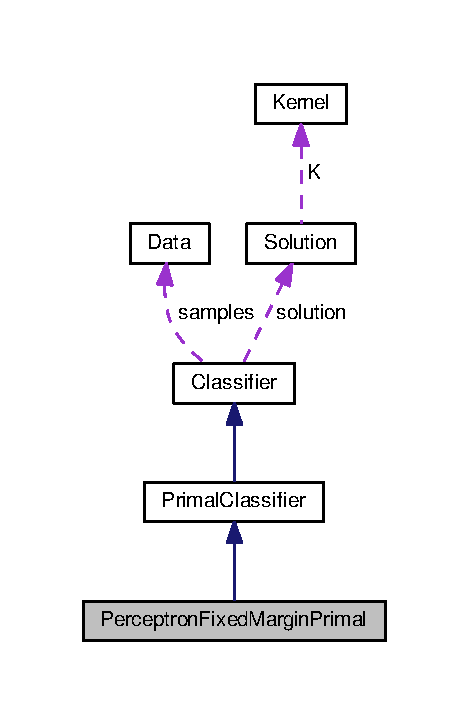
\includegraphics[width=225pt]{class_perceptron_fixed_margin_primal__coll__graph}
\end{center}
\end{figure}
\subsection*{Public Member Functions}
\begin{DoxyCompactItemize}
\item 
\mbox{\Hypertarget{class_perceptron_fixed_margin_primal_a0a0e3e5d302d640f7a66701e7166304d}\label{class_perceptron_fixed_margin_primal_a0a0e3e5d302d640f7a66701e7166304d}} 
{\bfseries Perceptron\+Fixed\+Margin\+Primal} (std\+::shared\+\_\+ptr$<$ \hyperlink{class_data}{Data} $>$ \hyperlink{class_classifier_aad6a4fcea8f44339d7a6302f530852ca}{samples}=nullptr, double gamma=1.\+0, double \hyperlink{class_primal_classifier_a746ad2ff93fb77d82ae389f90dbdc89e}{q}=2, double \hyperlink{class_classifier_af9867e5919742de1303dd971a9a1c19a}{rate}=0.\+5, \hyperlink{class_solution}{Solution} $\ast$initial\+\_\+solution=nullptr)
\item 
bool \hyperlink{class_perceptron_fixed_margin_primal_ad013cf0293dd8cda3ac751216b5a7f89}{train} () override
\begin{DoxyCompactList}\small\item\em Function that execute the training phase of a classification algorithm. \end{DoxyCompactList}\item 
double \hyperlink{class_perceptron_fixed_margin_primal_aa24b3bd358a438797c62fa13ef7b8872}{evaluate} (\hyperlink{class_point}{Point} p) override
\begin{DoxyCompactList}\small\item\em Returns the class of a feature point based on the trained classifier. \end{DoxyCompactList}\end{DoxyCompactItemize}
\subsection*{Additional Inherited Members}


\subsection{Detailed Description}
Wrapper for the implementation of the Perceptron primal with fixed margin algorithm. 

\subsection{Member Function Documentation}
\mbox{\Hypertarget{class_perceptron_fixed_margin_primal_aa24b3bd358a438797c62fa13ef7b8872}\label{class_perceptron_fixed_margin_primal_aa24b3bd358a438797c62fa13ef7b8872}} 
\index{Perceptron\+Fixed\+Margin\+Primal@{Perceptron\+Fixed\+Margin\+Primal}!evaluate@{evaluate}}
\index{evaluate@{evaluate}!Perceptron\+Fixed\+Margin\+Primal@{Perceptron\+Fixed\+Margin\+Primal}}
\subsubsection{\texorpdfstring{evaluate()}{evaluate()}}
{\footnotesize\ttfamily double Perceptron\+Fixed\+Margin\+Primal\+::evaluate (\begin{DoxyParamCaption}\item[{\hyperlink{class_point}{Point}}]{p }\end{DoxyParamCaption})\hspace{0.3cm}{\ttfamily [override]}, {\ttfamily [virtual]}}



Returns the class of a feature point based on the trained classifier. 


\begin{DoxyParams}{Parameters}
{\em \hyperlink{class_point}{Point}} & x (???) Features point to be evaluated. \\
\hline
\end{DoxyParams}
\begin{DoxyReturn}{Returns}
int 
\end{DoxyReturn}


Implements \hyperlink{class_classifier_ae8e9554823b85ddc2dcad2955da811d9}{Classifier}.

\mbox{\Hypertarget{class_perceptron_fixed_margin_primal_ad013cf0293dd8cda3ac751216b5a7f89}\label{class_perceptron_fixed_margin_primal_ad013cf0293dd8cda3ac751216b5a7f89}} 
\index{Perceptron\+Fixed\+Margin\+Primal@{Perceptron\+Fixed\+Margin\+Primal}!train@{train}}
\index{train@{train}!Perceptron\+Fixed\+Margin\+Primal@{Perceptron\+Fixed\+Margin\+Primal}}
\subsubsection{\texorpdfstring{train()}{train()}}
{\footnotesize\ttfamily bool Perceptron\+Fixed\+Margin\+Primal\+::train (\begin{DoxyParamCaption}{ }\end{DoxyParamCaption})\hspace{0.3cm}{\ttfamily [override]}, {\ttfamily [virtual]}}



Function that execute the training phase of a classification algorithm. 

\begin{DoxyReturn}{Returns}
void 
\end{DoxyReturn}


Implements \hyperlink{class_classifier_a2306a5de27555ab093593ac9642bc7d9}{Classifier}.



The documentation for this class was generated from the following files\+:\begin{DoxyCompactItemize}
\item 
includes/\hyperlink{_perceptron_8hpp}{Perceptron.\+hpp}\item 
src/Perceptron.\+cpp\end{DoxyCompactItemize}

\hypertarget{class_perceptron_primal}{}\section{Perceptron\+Primal Class Reference}
\label{class_perceptron_primal}\index{Perceptron\+Primal@{Perceptron\+Primal}}


Wrapper for the implementation of the Perceptron primal algorithm.  




{\ttfamily \#include $<$Perceptron.\+hpp$>$}



Inheritance diagram for Perceptron\+Primal\+:\nopagebreak
\begin{figure}[H]
\begin{center}
\leavevmode
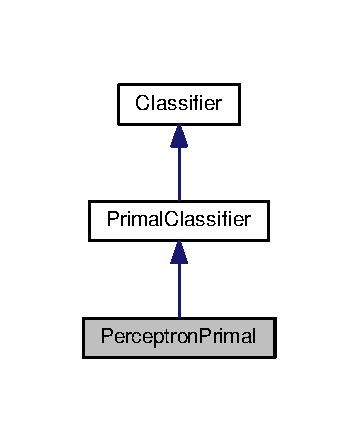
\includegraphics[width=172pt]{class_perceptron_primal__inherit__graph}
\end{center}
\end{figure}


Collaboration diagram for Perceptron\+Primal\+:\nopagebreak
\begin{figure}[H]
\begin{center}
\leavevmode
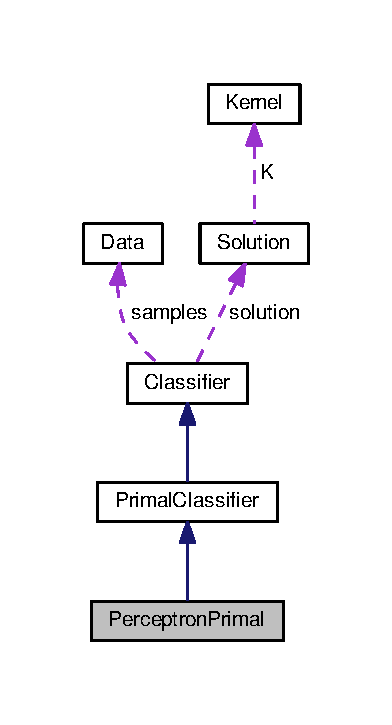
\includegraphics[width=188pt]{class_perceptron_primal__coll__graph}
\end{center}
\end{figure}
\subsection*{Public Member Functions}
\begin{DoxyCompactItemize}
\item 
\mbox{\Hypertarget{class_perceptron_primal_a3c182ca6be41096ac89aebcb45761660}\label{class_perceptron_primal_a3c182ca6be41096ac89aebcb45761660}} 
{\bfseries Perceptron\+Primal} (\hyperlink{class_data}{Data} $\ast$\hyperlink{class_classifier_a515c225d0da93df02ca79f9f87811d17}{samples}=N\+U\+LL, double \hyperlink{class_primal_classifier_a746ad2ff93fb77d82ae389f90dbdc89e}{q}=2, double \hyperlink{class_classifier_af9867e5919742de1303dd971a9a1c19a}{rate}=0.\+5, \hyperlink{class_solution}{Solution} $\ast$initial\+\_\+solution=N\+U\+LL)
\item 
bool \hyperlink{class_perceptron_primal_a17f817a72fc7d61d1686ea77f7f9e84d}{train} ()
\begin{DoxyCompactList}\small\item\em Function that execute the training phase of a classification algorithm. \end{DoxyCompactList}\item 
double \hyperlink{class_perceptron_primal_ac8ce9ceffe2b35b5386e5367fb419b3b}{evaluate} (\hyperlink{class_point}{Point} p)
\begin{DoxyCompactList}\small\item\em Returns the class of a feature point based on the trained classifier. \end{DoxyCompactList}\end{DoxyCompactItemize}
\subsection*{Additional Inherited Members}


\subsection{Detailed Description}
Wrapper for the implementation of the Perceptron primal algorithm. 

\subsection{Member Function Documentation}
\mbox{\Hypertarget{class_perceptron_primal_ac8ce9ceffe2b35b5386e5367fb419b3b}\label{class_perceptron_primal_ac8ce9ceffe2b35b5386e5367fb419b3b}} 
\index{Perceptron\+Primal@{Perceptron\+Primal}!evaluate@{evaluate}}
\index{evaluate@{evaluate}!Perceptron\+Primal@{Perceptron\+Primal}}
\subsubsection{\texorpdfstring{evaluate()}{evaluate()}}
{\footnotesize\ttfamily double Perceptron\+Primal\+::evaluate (\begin{DoxyParamCaption}\item[{\hyperlink{class_point}{Point}}]{p }\end{DoxyParamCaption})\hspace{0.3cm}{\ttfamily [virtual]}}



Returns the class of a feature point based on the trained classifier. 


\begin{DoxyParams}{Parameters}
{\em \hyperlink{class_point}{Point}} & x (???) Features point to be evaluated. \\
\hline
\end{DoxyParams}
\begin{DoxyReturn}{Returns}
int 
\end{DoxyReturn}


Implements \hyperlink{class_classifier_ae8e9554823b85ddc2dcad2955da811d9}{Classifier}.

\mbox{\Hypertarget{class_perceptron_primal_a17f817a72fc7d61d1686ea77f7f9e84d}\label{class_perceptron_primal_a17f817a72fc7d61d1686ea77f7f9e84d}} 
\index{Perceptron\+Primal@{Perceptron\+Primal}!train@{train}}
\index{train@{train}!Perceptron\+Primal@{Perceptron\+Primal}}
\subsubsection{\texorpdfstring{train()}{train()}}
{\footnotesize\ttfamily bool Perceptron\+Primal\+::train (\begin{DoxyParamCaption}{ }\end{DoxyParamCaption})\hspace{0.3cm}{\ttfamily [virtual]}}



Function that execute the training phase of a classification algorithm. 

\begin{DoxyReturn}{Returns}
void 
\end{DoxyReturn}


Implements \hyperlink{class_classifier_a2306a5de27555ab093593ac9642bc7d9}{Classifier}.



The documentation for this class was generated from the following files\+:\begin{DoxyCompactItemize}
\item 
includes/\hyperlink{_perceptron_8hpp}{Perceptron.\+hpp}\item 
src/Perceptron.\+cpp\end{DoxyCompactItemize}

\hypertarget{class_point}{}\section{Point Class Reference}
\label{class_point}\index{Point@{Point}}


Class of a \hyperlink{class_point}{Point} of doubles in a space of n dimensions.  




{\ttfamily \#include $<$Point.\+hpp$>$}

\subsection*{Public Member Functions}
\begin{DoxyCompactItemize}
\item 
\mbox{\Hypertarget{class_point_a82e69bcefbcbc72eac5c1acd88784aef}\label{class_point_a82e69bcefbcbc72eac5c1acd88784aef}} 
{\bfseries Point} (int dim)
\item 
double \hyperlink{class_point_a9d8da6733d7e4110a62e8d0f82676761}{dot} (std\+::vector$<$ double $>$ p)
\begin{DoxyCompactList}\small\item\em Computes the dot product with a vector. \end{DoxyCompactList}\item 
double \hyperlink{class_point_aab64e3f0a9eecba00a1607eb4c7768c3}{norm} (int p=2)
\begin{DoxyCompactList}\small\item\em Returns the p-\/norm of the point. \end{DoxyCompactList}\end{DoxyCompactItemize}
\subsection*{Public Attributes}
\begin{DoxyCompactItemize}
\item 
\mbox{\Hypertarget{class_point_a1e22056737f10e31025b353c86e3b9e3}\label{class_point_a1e22056737f10e31025b353c86e3b9e3}} 
std\+::vector$<$ double $>$ \hyperlink{class_point_a1e22056737f10e31025b353c86e3b9e3}{x}
\begin{DoxyCompactList}\small\item\em Features values. \end{DoxyCompactList}\item 
\mbox{\Hypertarget{class_point_afa38be143ae800e6ad69ce8ed4df62d8}\label{class_point_afa38be143ae800e6ad69ce8ed4df62d8}} 
double \hyperlink{class_point_afa38be143ae800e6ad69ce8ed4df62d8}{y} = 0
\begin{DoxyCompactList}\small\item\em \hyperlink{class_point}{Point} classification. \end{DoxyCompactList}\item 
\mbox{\Hypertarget{class_point_a8595ba929b962c97293ab35a0c60b434}\label{class_point_a8595ba929b962c97293ab35a0c60b434}} 
double {\bfseries alpha} = 0.\+0
\item 
\mbox{\Hypertarget{class_point_a3ccd2080027d6845744bd044280da9e7}\label{class_point_a3ccd2080027d6845744bd044280da9e7}} 
int \hyperlink{class_point_a3ccd2080027d6845744bd044280da9e7}{id} = 0
\begin{DoxyCompactList}\small\item\em \hyperlink{class_point}{Point} identification. \end{DoxyCompactList}\end{DoxyCompactItemize}
\subsection*{Friends}
\begin{DoxyCompactItemize}
\item 
\mbox{\Hypertarget{class_point_a18e1e2eb3b3b27719f367688e8611b45}\label{class_point_a18e1e2eb3b3b27719f367688e8611b45}} 
std\+::ostream \& {\bfseries operator$<$$<$} (std\+::ostream \&output, const \hyperlink{class_point}{Point} \&p)
\end{DoxyCompactItemize}


\subsection{Detailed Description}
Class of a \hyperlink{class_point}{Point} of doubles in a space of n dimensions. 

\subsection{Member Function Documentation}
\mbox{\Hypertarget{class_point_a9d8da6733d7e4110a62e8d0f82676761}\label{class_point_a9d8da6733d7e4110a62e8d0f82676761}} 
\index{Point@{Point}!dot@{dot}}
\index{dot@{dot}!Point@{Point}}
\subsubsection{\texorpdfstring{dot()}{dot()}}
{\footnotesize\ttfamily double Point\+::dot (\begin{DoxyParamCaption}\item[{std\+::vector$<$ double $>$}]{p }\end{DoxyParamCaption})}



Computes the dot product with a vector. 


\begin{DoxyParams}{Parameters}
{\em p} & (???) \\
\hline
\end{DoxyParams}
\begin{DoxyReturn}{Returns}
double 
\end{DoxyReturn}
\mbox{\Hypertarget{class_point_aab64e3f0a9eecba00a1607eb4c7768c3}\label{class_point_aab64e3f0a9eecba00a1607eb4c7768c3}} 
\index{Point@{Point}!norm@{norm}}
\index{norm@{norm}!Point@{Point}}
\subsubsection{\texorpdfstring{norm()}{norm()}}
{\footnotesize\ttfamily double Point\+::norm (\begin{DoxyParamCaption}\item[{int}]{p = {\ttfamily 2} }\end{DoxyParamCaption})}



Returns the p-\/norm of the point. 


\begin{DoxyParams}{Parameters}
{\em p} & (???) p of the norm (euclidean norm is the default). \\
\hline
\end{DoxyParams}
\begin{DoxyReturn}{Returns}
double 
\end{DoxyReturn}


The documentation for this class was generated from the following files\+:\begin{DoxyCompactItemize}
\item 
includes/Point.\+hpp\item 
src/\hyperlink{_point_8cpp}{Point.\+cpp}\end{DoxyCompactItemize}

\hypertarget{class_primal_classifier}{}\section{Primal\+Classifier$<$ T $>$ Class Template Reference}
\label{class_primal_classifier}\index{Primal\+Classifier$<$ T $>$@{Primal\+Classifier$<$ T $>$}}


Inheritance diagram for Primal\+Classifier$<$ T $>$\+:
% FIG 0


Collaboration diagram for Primal\+Classifier$<$ T $>$\+:
% FIG 1
\subsection*{Public Member Functions}
\begin{DoxyCompactItemize}
\item 
std\+::string \mbox{\hyperlink{class_primal_classifier_a637fc3cb89994277e902758c7fc3f763}{classifier\+Type}} ()
\begin{DoxyCompactList}\small\item\em Returns the type of the classifier. \end{DoxyCompactList}\item 
void \mbox{\hyperlink{class_primal_classifier_a7e6953c01b190e6ef968b75bd578ad7d}{setq\+Norm}} (double \mbox{\hyperlink{class_primal_classifier_ae30c00c25bce4b1623baa54b5e2812b4}{q}})
\begin{DoxyCompactList}\small\item\em setq\+Norm Set the q norm used by the classifier. (Euclidean norm is the default) \end{DoxyCompactList}\item 
void \mbox{\hyperlink{class_primal_classifier_ad0c3b7577b6c11da7394105dd2002f1d}{setp\+Norm}} (double p)
\begin{DoxyCompactList}\small\item\em setp\+Norm Set the p norm used by the classifier. (Euclidean norm is the default) \end{DoxyCompactList}\item 
void \mbox{\hyperlink{class_primal_classifier_a7e5c459cb4a377c794502cd9831ee095}{set\+Flexible}} (double \mbox{\hyperlink{class_primal_classifier_a5d41554dc1158ede39d387fecf73c96e}{flexible}})
\begin{DoxyCompactList}\small\item\em Set flexibity of the classifier. \end{DoxyCompactList}\item 
void \mbox{\hyperlink{class_primal_classifier_a049f4814d38b456c80c40cee5595502b}{set\+Alpha\+Aprox}} (double \mbox{\hyperlink{class_primal_classifier_a2668546ac4a39e10f72cbd2e865c41a7}{alpha\+\_\+aprox}})
\begin{DoxyCompactList}\small\item\em Set the percentage of the aproximation. \end{DoxyCompactList}\end{DoxyCompactItemize}
\subsection*{Protected Attributes}
\begin{DoxyCompactItemize}
\item 
\mbox{\Hypertarget{class_primal_classifier_a6191919f25a037b6a61d00ebda18f41e}\label{class_primal_classifier_a6191919f25a037b6a61d00ebda18f41e}} 
std\+::vector$<$ double $>$ \mbox{\hyperlink{class_primal_classifier_a6191919f25a037b6a61d00ebda18f41e}{w}}
\begin{DoxyCompactList}\small\item\em Weights vector. \end{DoxyCompactList}\item 
\mbox{\Hypertarget{class_primal_classifier_ae30c00c25bce4b1623baa54b5e2812b4}\label{class_primal_classifier_ae30c00c25bce4b1623baa54b5e2812b4}} 
double \mbox{\hyperlink{class_primal_classifier_ae30c00c25bce4b1623baa54b5e2812b4}{q}} = 2
\begin{DoxyCompactList}\small\item\em Norm used in the classification. (Euclidean Norm is the default) \end{DoxyCompactList}\item 
\mbox{\Hypertarget{class_primal_classifier_ac5b59dafe749376fb067ceda690f405d}\label{class_primal_classifier_ac5b59dafe749376fb067ceda690f405d}} 
double {\bfseries p} = 2
\item 
\mbox{\Hypertarget{class_primal_classifier_a5d41554dc1158ede39d387fecf73c96e}\label{class_primal_classifier_a5d41554dc1158ede39d387fecf73c96e}} 
double \mbox{\hyperlink{class_primal_classifier_a5d41554dc1158ede39d387fecf73c96e}{flexible}} = 0.\+0
\begin{DoxyCompactList}\small\item\em Flexibility. \end{DoxyCompactList}\item 
\mbox{\Hypertarget{class_primal_classifier_a2668546ac4a39e10f72cbd2e865c41a7}\label{class_primal_classifier_a2668546ac4a39e10f72cbd2e865c41a7}} 
double \mbox{\hyperlink{class_primal_classifier_a2668546ac4a39e10f72cbd2e865c41a7}{alpha\+\_\+aprox}} = 0.\+0
\begin{DoxyCompactList}\small\item\em Percentage of aproximation of the result. \end{DoxyCompactList}\end{DoxyCompactItemize}


\subsection{Member Function Documentation}
\mbox{\Hypertarget{class_primal_classifier_a637fc3cb89994277e902758c7fc3f763}\label{class_primal_classifier_a637fc3cb89994277e902758c7fc3f763}} 
\index{Primal\+Classifier@{Primal\+Classifier}!classifier\+Type@{classifier\+Type}}
\index{classifier\+Type@{classifier\+Type}!Primal\+Classifier@{Primal\+Classifier}}
\subsubsection{\texorpdfstring{classifier\+Type()}{classifierType()}}
{\footnotesize\ttfamily template$<$typename T $>$ \\
std\+::string \mbox{\hyperlink{class_primal_classifier}{Primal\+Classifier}}$<$ T $>$\+::classifier\+Type (\begin{DoxyParamCaption}{ }\end{DoxyParamCaption})\hspace{0.3cm}{\ttfamily [inline]}, {\ttfamily [virtual]}}



Returns the type of the classifier. 

\begin{DoxyReturn}{Returns}
std\+::string 
\end{DoxyReturn}


Implements \mbox{\hyperlink{class_classifier_ab40f42f957ec50939bd9a6b0cd5d1786}{Classifier$<$ T $>$}}.

\mbox{\Hypertarget{class_primal_classifier_a049f4814d38b456c80c40cee5595502b}\label{class_primal_classifier_a049f4814d38b456c80c40cee5595502b}} 
\index{Primal\+Classifier@{Primal\+Classifier}!set\+Alpha\+Aprox@{set\+Alpha\+Aprox}}
\index{set\+Alpha\+Aprox@{set\+Alpha\+Aprox}!Primal\+Classifier@{Primal\+Classifier}}
\subsubsection{\texorpdfstring{set\+Alpha\+Aprox()}{setAlphaAprox()}}
{\footnotesize\ttfamily template$<$typename T $>$ \\
void \mbox{\hyperlink{class_primal_classifier}{Primal\+Classifier}}$<$ T $>$\+::set\+Alpha\+Aprox (\begin{DoxyParamCaption}\item[{double}]{alpha\+\_\+aprox }\end{DoxyParamCaption})\hspace{0.3cm}{\ttfamily [inline]}}



Set the percentage of the aproximation. 


\begin{DoxyParams}{Parameters}
{\em alpha\+\_\+aprox} & Aproximation. \\
\hline
\end{DoxyParams}
\mbox{\Hypertarget{class_primal_classifier_a7e5c459cb4a377c794502cd9831ee095}\label{class_primal_classifier_a7e5c459cb4a377c794502cd9831ee095}} 
\index{Primal\+Classifier@{Primal\+Classifier}!set\+Flexible@{set\+Flexible}}
\index{set\+Flexible@{set\+Flexible}!Primal\+Classifier@{Primal\+Classifier}}
\subsubsection{\texorpdfstring{set\+Flexible()}{setFlexible()}}
{\footnotesize\ttfamily template$<$typename T $>$ \\
void \mbox{\hyperlink{class_primal_classifier}{Primal\+Classifier}}$<$ T $>$\+::set\+Flexible (\begin{DoxyParamCaption}\item[{double}]{flexible }\end{DoxyParamCaption})\hspace{0.3cm}{\ttfamily [inline]}}



Set flexibity of the classifier. 


\begin{DoxyParams}{Parameters}
{\em flexible} & flexibility. \\
\hline
\end{DoxyParams}
\mbox{\Hypertarget{class_primal_classifier_ad0c3b7577b6c11da7394105dd2002f1d}\label{class_primal_classifier_ad0c3b7577b6c11da7394105dd2002f1d}} 
\index{Primal\+Classifier@{Primal\+Classifier}!setp\+Norm@{setp\+Norm}}
\index{setp\+Norm@{setp\+Norm}!Primal\+Classifier@{Primal\+Classifier}}
\subsubsection{\texorpdfstring{setp\+Norm()}{setpNorm()}}
{\footnotesize\ttfamily template$<$typename T $>$ \\
void \mbox{\hyperlink{class_primal_classifier}{Primal\+Classifier}}$<$ T $>$\+::setp\+Norm (\begin{DoxyParamCaption}\item[{double}]{p }\end{DoxyParamCaption})\hspace{0.3cm}{\ttfamily [inline]}}



setp\+Norm Set the p norm used by the classifier. (Euclidean norm is the default) 


\begin{DoxyParams}{Parameters}
{\em p} & Norm that will be used by the classifier. \\
\hline
\end{DoxyParams}
\mbox{\Hypertarget{class_primal_classifier_a7e6953c01b190e6ef968b75bd578ad7d}\label{class_primal_classifier_a7e6953c01b190e6ef968b75bd578ad7d}} 
\index{Primal\+Classifier@{Primal\+Classifier}!setq\+Norm@{setq\+Norm}}
\index{setq\+Norm@{setq\+Norm}!Primal\+Classifier@{Primal\+Classifier}}
\subsubsection{\texorpdfstring{setq\+Norm()}{setqNorm()}}
{\footnotesize\ttfamily template$<$typename T $>$ \\
void \mbox{\hyperlink{class_primal_classifier}{Primal\+Classifier}}$<$ T $>$\+::setq\+Norm (\begin{DoxyParamCaption}\item[{double}]{q }\end{DoxyParamCaption})\hspace{0.3cm}{\ttfamily [inline]}}



setq\+Norm Set the q norm used by the classifier. (Euclidean norm is the default) 


\begin{DoxyParams}{Parameters}
{\em q} & Norm that will be used by the classifier. \\
\hline
\end{DoxyParams}


The documentation for this class was generated from the following file\+:\begin{DoxyCompactItemize}
\item 
includes/\mbox{\hyperlink{_primal_classifier_8hpp}{Primal\+Classifier.\+hpp}}\end{DoxyCompactItemize}

\hypertarget{class_solution}{}\section{Solution Class Reference}
\label{class_solution}\index{Solution@{Solution}}


Inheritance diagram for Solution\+:\nopagebreak
\begin{figure}[H]
\begin{center}
\leavevmode
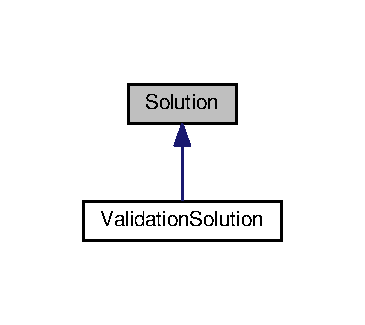
\includegraphics[width=175pt]{class_solution__inherit__graph}
\end{center}
\end{figure}
\subsection*{Public Attributes}
\begin{DoxyCompactItemize}
\item 
\mbox{\Hypertarget{class_solution_a736054c66aab1014bba4a71de293ad2f}\label{class_solution_a736054c66aab1014bba4a71de293ad2f}} 
std\+::vector$<$ double $>$ \hyperlink{class_solution_a736054c66aab1014bba4a71de293ad2f}{w}
\begin{DoxyCompactList}\small\item\em Weights vector. \end{DoxyCompactList}\item 
\mbox{\Hypertarget{class_solution_ac0a589a77d238aecf14c91f55d1b8daa}\label{class_solution_ac0a589a77d238aecf14c91f55d1b8daa}} 
double \hyperlink{class_solution_ac0a589a77d238aecf14c91f55d1b8daa}{bias} = 0
\begin{DoxyCompactList}\small\item\em Bias of the solution. \end{DoxyCompactList}\item 
\mbox{\Hypertarget{class_solution_a86d40d16bfa9e7dbe476a62008431987}\label{class_solution_a86d40d16bfa9e7dbe476a62008431987}} 
std\+::vector$<$ int $>$ \hyperlink{class_solution_a86d40d16bfa9e7dbe476a62008431987}{fnames}
\begin{DoxyCompactList}\small\item\em Features names of the resulting solution. \end{DoxyCompactList}\item 
\mbox{\Hypertarget{class_solution_a3580af26a22d86e44df701f654165e0f}\label{class_solution_a3580af26a22d86e44df701f654165e0f}} 
double \hyperlink{class_solution_a3580af26a22d86e44df701f654165e0f}{margin} = 0
\begin{DoxyCompactList}\small\item\em Margin generated from the classifier that generated the solution. \end{DoxyCompactList}\item 
\mbox{\Hypertarget{class_solution_acbc0610c1c2e2d7bb5c39af33b7eb99c}\label{class_solution_acbc0610c1c2e2d7bb5c39af33b7eb99c}} 
double \hyperlink{class_solution_acbc0610c1c2e2d7bb5c39af33b7eb99c}{norm} = 0
\begin{DoxyCompactList}\small\item\em Norm of the solution. \end{DoxyCompactList}\end{DoxyCompactItemize}


The documentation for this class was generated from the following file\+:\begin{DoxyCompactItemize}
\item 
includes/Solution.\+hpp\end{DoxyCompactItemize}

\hypertarget{class_statistics}{}\section{Statistics Class Reference}
\label{class_statistics}\index{Statistics@{Statistics}}


Class with methods for statistical computations.  




{\ttfamily \#include $<$Statistics.\+hpp$>$}



Collaboration diagram for Statistics\+:\nopagebreak
\begin{figure}[H]
\begin{center}
\leavevmode
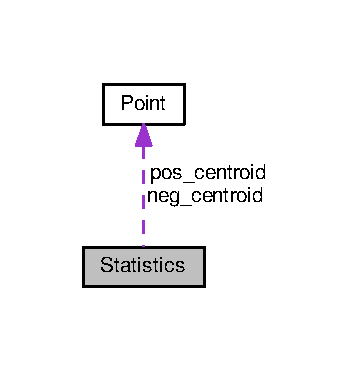
\includegraphics[width=168pt]{class_statistics__coll__graph}
\end{center}
\end{figure}
\subsection*{Static Public Member Functions}
\begin{DoxyCompactItemize}
\item 
static double \hyperlink{class_statistics_a4c1ba6a34efe8686419edd83e7c6d579}{stdev} (std\+::vector$<$ double $>$ p)
\begin{DoxyCompactList}\small\item\em Compute the standard deviation of a vector. \end{DoxyCompactList}\item 
static double \hyperlink{class_statistics_ad56432dac5366707268de10e58f7972a}{mean} (std\+::vector$<$ double $>$ p)
\begin{DoxyCompactList}\small\item\em Compute the mean (average) of a vector. \end{DoxyCompactList}\end{DoxyCompactItemize}
\subsection*{Public Attributes}
\begin{DoxyCompactItemize}
\item 
\mbox{\Hypertarget{class_statistics_a51adeaf4b7f078a4dfd373082fd1f7e1}\label{class_statistics_a51adeaf4b7f078a4dfd373082fd1f7e1}} 
\hyperlink{class_point}{Point} \hyperlink{class_statistics_a51adeaf4b7f078a4dfd373082fd1f7e1}{pos\+\_\+centroid}
\begin{DoxyCompactList}\small\item\em Centroid of the positive points. \end{DoxyCompactList}\item 
\mbox{\Hypertarget{class_statistics_ab7a104abc574d7d0e063f97ccc5f52e0}\label{class_statistics_ab7a104abc574d7d0e063f97ccc5f52e0}} 
\hyperlink{class_point}{Point} \hyperlink{class_statistics_ab7a104abc574d7d0e063f97ccc5f52e0}{neg\+\_\+centroid}
\begin{DoxyCompactList}\small\item\em Centroid of the negative points. \end{DoxyCompactList}\item 
\mbox{\Hypertarget{class_statistics_a95918ee9568c41b665ba3920f3255829}\label{class_statistics_a95918ee9568c41b665ba3920f3255829}} 
int \hyperlink{class_statistics_a95918ee9568c41b665ba3920f3255829}{n\+\_\+pos} = 0
\begin{DoxyCompactList}\small\item\em Number of positive points. \end{DoxyCompactList}\item 
\mbox{\Hypertarget{class_statistics_a221eee7599d594bc55f69608c82bb242}\label{class_statistics_a221eee7599d594bc55f69608c82bb242}} 
int \hyperlink{class_statistics_a221eee7599d594bc55f69608c82bb242}{n\+\_\+neg} = 0
\begin{DoxyCompactList}\small\item\em Number of negative points. \end{DoxyCompactList}\end{DoxyCompactItemize}


\subsection{Detailed Description}
Class with methods for statistical computations. 

\subsection{Member Function Documentation}
\mbox{\Hypertarget{class_statistics_ad56432dac5366707268de10e58f7972a}\label{class_statistics_ad56432dac5366707268de10e58f7972a}} 
\index{Statistics@{Statistics}!mean@{mean}}
\index{mean@{mean}!Statistics@{Statistics}}
\subsubsection{\texorpdfstring{mean()}{mean()}}
{\footnotesize\ttfamily static double Statistics\+::mean (\begin{DoxyParamCaption}\item[{std\+::vector$<$ double $>$}]{p }\end{DoxyParamCaption})\hspace{0.3cm}{\ttfamily [static]}}



Compute the mean (average) of a vector. 


\begin{DoxyParams}{Parameters}
{\em p} & (???) \hyperlink{class_point}{Point} to compute the mean. \\
\hline
\end{DoxyParams}
\begin{DoxyReturn}{Returns}
double 
\end{DoxyReturn}
\mbox{\Hypertarget{class_statistics_a4c1ba6a34efe8686419edd83e7c6d579}\label{class_statistics_a4c1ba6a34efe8686419edd83e7c6d579}} 
\index{Statistics@{Statistics}!stdev@{stdev}}
\index{stdev@{stdev}!Statistics@{Statistics}}
\subsubsection{\texorpdfstring{stdev()}{stdev()}}
{\footnotesize\ttfamily static double Statistics\+::stdev (\begin{DoxyParamCaption}\item[{std\+::vector$<$ double $>$}]{p }\end{DoxyParamCaption})\hspace{0.3cm}{\ttfamily [static]}}



Compute the standard deviation of a vector. 


\begin{DoxyParams}{Parameters}
{\em p} & (???) \hyperlink{class_point}{Point} to compute stdev. \\
\hline
\end{DoxyParams}
\begin{DoxyReturn}{Returns}
double 
\end{DoxyReturn}


The documentation for this class was generated from the following file\+:\begin{DoxyCompactItemize}
\item 
/home/mateus558/\+Dropbox/\+Aprendizado de Máquinas/\+Classification\+\_\+\+Algorithms\+\_\+\+System/includes/Statistics.\+hpp\end{DoxyCompactItemize}

\hypertarget{class_timer}{}\section{Timer Class Reference}
\label{class_timer}\index{Timer@{Timer}}


Wrapper for the implementation of a simple timer.  




{\ttfamily \#include $<$Timer.\+hpp$>$}

\subsection*{Public Member Functions}
\begin{DoxyCompactItemize}
\item 
\hyperlink{class_timer_a5f16e8da27d2a5a5242dead46de05d97}{Timer} ()\hypertarget{class_timer_a5f16e8da27d2a5a5242dead46de05d97}{}\label{class_timer_a5f16e8da27d2a5a5242dead46de05d97}

\begin{DoxyCompactList}\small\item\em Contructor already initiate the timer to the current time. \end{DoxyCompactList}\item 
void \hyperlink{class_timer_ae7c0c1e7d12de4b8a6e7c64e451cdd2a}{Reset} ()\hypertarget{class_timer_ae7c0c1e7d12de4b8a6e7c64e451cdd2a}{}\label{class_timer_ae7c0c1e7d12de4b8a6e7c64e451cdd2a}

\begin{DoxyCompactList}\small\item\em Set the timer to the current time. \end{DoxyCompactList}\item 
double \hyperlink{class_timer_a8bb6cb4f5813c7a3aea3c37f8bcbf0ea}{Elapsed} () const 
\begin{DoxyCompactList}\small\item\em Returns the elapsed time. \end{DoxyCompactList}\end{DoxyCompactItemize}


\subsection{Detailed Description}
Wrapper for the implementation of a simple timer. 

\subsection{Member Function Documentation}
\index{Timer@{Timer}!Elapsed@{Elapsed}}
\index{Elapsed@{Elapsed}!Timer@{Timer}}
\subsubsection[{\texorpdfstring{Elapsed() const }{Elapsed() const }}]{\setlength{\rightskip}{0pt plus 5cm}double Timer\+::\+Elapsed (
\begin{DoxyParamCaption}
{}
\end{DoxyParamCaption}
) const\hspace{0.3cm}{\ttfamily [inline]}}\hypertarget{class_timer_a8bb6cb4f5813c7a3aea3c37f8bcbf0ea}{}\label{class_timer_a8bb6cb4f5813c7a3aea3c37f8bcbf0ea}


Returns the elapsed time. 

\begin{DoxyReturn}{Returns}
double 
\end{DoxyReturn}


The documentation for this class was generated from the following file\+:\begin{DoxyCompactItemize}
\item 
includes/\hyperlink{_timer_8hpp}{Timer.\+hpp}\end{DoxyCompactItemize}

\hypertarget{class_validation}{}\section{Validation$<$ T $>$ Class Template Reference}
\label{class_validation}\index{Validation$<$ T $>$@{Validation$<$ T $>$}}


Class of methods for the validation of ML algorithms.  




{\ttfamily \#include $<$Validation.\+hpp$>$}

\subsection*{Classes}
\begin{DoxyCompactItemize}
\item 
struct \hyperlink{struct_validation_1_1_cross_validation}{Cross\+Validation}
\end{DoxyCompactItemize}
\subsection*{Public Member Functions}
\begin{DoxyCompactItemize}
\item 
\mbox{\Hypertarget{class_validation_a26fec6a8582bded0583a4754cdba0009}\label{class_validation_a26fec6a8582bded0583a4754cdba0009}} 
void {\bfseries set\+Seed} (unsigned int seed)
\item 
\mbox{\Hypertarget{class_validation_a8421390022d90bebecf761d23533c72e}\label{class_validation_a8421390022d90bebecf761d23533c72e}} 
\hyperlink{class_validation_a8421390022d90bebecf761d23533c72e}{Validation} ()
\begin{DoxyCompactList}\small\item\em Default constructor. \end{DoxyCompactList}\item 
\hyperlink{class_validation_a91399f8b544cb22de02b85618ef5b0cc}{Validation} (std\+::shared\+\_\+ptr$<$ \hyperlink{class_data}{Data}$<$ T $>$ $>$ sample=std\+::make\+\_\+shared$<$ \hyperlink{class_data}{Data}$<$ T $>$ $>$(), \hyperlink{class_classifier}{Classifier}$<$ T $>$ $\ast$classifier=nullptr, unsigned int seed=666)
\begin{DoxyCompactList}\small\item\em Constructor initializing the sample and classifier used. \end{DoxyCompactList}\item 
void \hyperlink{class_validation_a1e9580697a164d4bfbe721f2f1589c57}{part\+Train\+Test} (int fold)
\begin{DoxyCompactList}\small\item\em Executes the Stratified K-\/fold algorithm. \end{DoxyCompactList}\item 
double \hyperlink{class_validation_a1a5825e2dd051a72aaffd423a0df55f1}{k\+Fold} (int fold, int seed)
\begin{DoxyCompactList}\small\item\em Executes the k. \end{DoxyCompactList}\item 
double \hyperlink{class_validation_a94a4eef1571e6e2665d7e8d5df7b20c6}{validation} (int fold, int qtde)
\begin{DoxyCompactList}\small\item\em Executes the validation with several executions of the k fold algorithm. \end{DoxyCompactList}\item 
std\+::shared\+\_\+ptr$<$ \hyperlink{class_data}{Data}$<$ T $>$ $>$ \hyperlink{class_validation_a2370445658f5e86e39e8c18fc8b971d0}{get\+Test\+Sample} ()
\begin{DoxyCompactList}\small\item\em Get the train sample used in the validation of the model. \end{DoxyCompactList}\item 
std\+::shared\+\_\+ptr$<$ \hyperlink{class_data}{Data}$<$ T $>$ $>$ \hyperlink{class_validation_a11cf518681b25799f231ce973ad45095}{get\+Train\+Sample} ()
\begin{DoxyCompactList}\small\item\em Get the train sample used in the validation of the model. \end{DoxyCompactList}\item 
void \hyperlink{class_validation_adddf2e9eb960b7636e6615ecbd9783bb}{set\+Verbose} (int verbose)
\begin{DoxyCompactList}\small\item\em Set the verbose. \end{DoxyCompactList}\end{DoxyCompactItemize}


\subsection{Detailed Description}
\subsubsection*{template$<$typename T$>$\newline
class Validation$<$ T $>$}

Class of methods for the validation of ML algorithms. 

\subsection{Constructor \& Destructor Documentation}
\mbox{\Hypertarget{class_validation_a91399f8b544cb22de02b85618ef5b0cc}\label{class_validation_a91399f8b544cb22de02b85618ef5b0cc}} 
\index{Validation@{Validation}!Validation@{Validation}}
\index{Validation@{Validation}!Validation@{Validation}}
\subsubsection{\texorpdfstring{Validation()}{Validation()}}
{\footnotesize\ttfamily template$<$typename T $>$ \\
\hyperlink{class_validation}{Validation}$<$ T $>$\+::\hyperlink{class_validation}{Validation} (\begin{DoxyParamCaption}\item[{std\+::shared\+\_\+ptr$<$ \hyperlink{class_data}{Data}$<$ T $>$ $>$}]{sample = {\ttfamily std\+:\+:make\+\_\+shared$<$\hyperlink{class_data}{Data}$<$~T~$>$~$>$()},  }\item[{\hyperlink{class_classifier}{Classifier}$<$ T $>$ $\ast$}]{classifier = {\ttfamily nullptr},  }\item[{unsigned int}]{seed = {\ttfamily 666} }\end{DoxyParamCaption})\hspace{0.3cm}{\ttfamily [explicit]}}



Constructor initializing the sample and classifier used. 


\begin{DoxyParams}{Parameters}
{\em sample} & Sample to be used in the validation. \\
\hline
{\em classifier} & Model to be validated. \\
\hline
{\em seed} & Seed to feed the pseudo random number generator. \\
\hline
\end{DoxyParams}


\subsection{Member Function Documentation}
\mbox{\Hypertarget{class_validation_a2370445658f5e86e39e8c18fc8b971d0}\label{class_validation_a2370445658f5e86e39e8c18fc8b971d0}} 
\index{Validation@{Validation}!get\+Test\+Sample@{get\+Test\+Sample}}
\index{get\+Test\+Sample@{get\+Test\+Sample}!Validation@{Validation}}
\subsubsection{\texorpdfstring{get\+Test\+Sample()}{getTestSample()}}
{\footnotesize\ttfamily template$<$typename T $>$ \\
std\+::shared\+\_\+ptr$<$ \hyperlink{class_data}{Data}$<$ T $>$ $>$ \hyperlink{class_validation}{Validation}$<$ T $>$\+::get\+Test\+Sample (\begin{DoxyParamCaption}{ }\end{DoxyParamCaption})}



Get the train sample used in the validation of the model. 

\begin{DoxyReturn}{Returns}
\hyperlink{class_data}{Data} 
\end{DoxyReturn}
\mbox{\Hypertarget{class_validation_a11cf518681b25799f231ce973ad45095}\label{class_validation_a11cf518681b25799f231ce973ad45095}} 
\index{Validation@{Validation}!get\+Train\+Sample@{get\+Train\+Sample}}
\index{get\+Train\+Sample@{get\+Train\+Sample}!Validation@{Validation}}
\subsubsection{\texorpdfstring{get\+Train\+Sample()}{getTrainSample()}}
{\footnotesize\ttfamily template$<$typename T $>$ \\
std\+::shared\+\_\+ptr$<$ \hyperlink{class_data}{Data}$<$ T $>$ $>$ \hyperlink{class_validation}{Validation}$<$ T $>$\+::get\+Train\+Sample (\begin{DoxyParamCaption}{ }\end{DoxyParamCaption})}



Get the train sample used in the validation of the model. 

\begin{DoxyReturn}{Returns}
\hyperlink{class_data}{Data} 
\end{DoxyReturn}
\mbox{\Hypertarget{class_validation_a1a5825e2dd051a72aaffd423a0df55f1}\label{class_validation_a1a5825e2dd051a72aaffd423a0df55f1}} 
\index{Validation@{Validation}!k\+Fold@{k\+Fold}}
\index{k\+Fold@{k\+Fold}!Validation@{Validation}}
\subsubsection{\texorpdfstring{k\+Fold()}{kFold()}}
{\footnotesize\ttfamily template$<$typename T $>$ \\
double \hyperlink{class_validation}{Validation}$<$ T $>$\+::k\+Fold (\begin{DoxyParamCaption}\item[{int}]{fold,  }\item[{int}]{seed }\end{DoxyParamCaption})}



Executes the k. 


\begin{DoxyParams}{Parameters}
{\em fold} & Number of folds. \\
\hline
{\em seed} & Seed to feed the pseudo random number generator. \\
\hline
\end{DoxyParams}
\mbox{\Hypertarget{class_validation_a1e9580697a164d4bfbe721f2f1589c57}\label{class_validation_a1e9580697a164d4bfbe721f2f1589c57}} 
\index{Validation@{Validation}!part\+Train\+Test@{part\+Train\+Test}}
\index{part\+Train\+Test@{part\+Train\+Test}!Validation@{Validation}}
\subsubsection{\texorpdfstring{part\+Train\+Test()}{partTrainTest()}}
{\footnotesize\ttfamily template$<$typename T $>$ \\
void \hyperlink{class_validation}{Validation}$<$ T $>$\+::part\+Train\+Test (\begin{DoxyParamCaption}\item[{int}]{fold }\end{DoxyParamCaption})}



Executes the Stratified K-\/fold algorithm. 


\begin{DoxyParams}{Parameters}
{\em fold} & Number of folds. \\
\hline
\end{DoxyParams}
\mbox{\Hypertarget{class_validation_adddf2e9eb960b7636e6615ecbd9783bb}\label{class_validation_adddf2e9eb960b7636e6615ecbd9783bb}} 
\index{Validation@{Validation}!set\+Verbose@{set\+Verbose}}
\index{set\+Verbose@{set\+Verbose}!Validation@{Validation}}
\subsubsection{\texorpdfstring{set\+Verbose()}{setVerbose()}}
{\footnotesize\ttfamily template$<$typename T $>$ \\
void \hyperlink{class_validation}{Validation}$<$ T $>$\+::set\+Verbose (\begin{DoxyParamCaption}\item[{int}]{verbose }\end{DoxyParamCaption})\hspace{0.3cm}{\ttfamily [inline]}}



Set the verbose. 


\begin{DoxyParams}{Parameters}
{\em verbose} & Verbose level. \\
\hline
\end{DoxyParams}
\mbox{\Hypertarget{class_validation_a94a4eef1571e6e2665d7e8d5df7b20c6}\label{class_validation_a94a4eef1571e6e2665d7e8d5df7b20c6}} 
\index{Validation@{Validation}!validation@{validation}}
\index{validation@{validation}!Validation@{Validation}}
\subsubsection{\texorpdfstring{validation()}{validation()}}
{\footnotesize\ttfamily template$<$typename T $>$ \\
double \hyperlink{class_validation}{Validation}$<$ T $>$\+::validation (\begin{DoxyParamCaption}\item[{int}]{fold,  }\item[{int}]{qtde }\end{DoxyParamCaption})}



Executes the validation with several executions of the k fold algorithm. 


\begin{DoxyParams}{Parameters}
{\em fold} & Number of folds. \\
\hline
{\em qtde} & Number of executions. \\
\hline
\end{DoxyParams}
\begin{DoxyReturn}{Returns}
double \hyperlink{class_validation}{Validation} error. 
\end{DoxyReturn}


The documentation for this class was generated from the following files\+:\begin{DoxyCompactItemize}
\item 
includes/Validation.\+hpp\item 
src/Validation.\+cpp\end{DoxyCompactItemize}

\hypertarget{class_validation_solution}{}\section{Validation\+Solution Class Reference}
\label{class_validation_solution}\index{Validation\+Solution@{Validation\+Solution}}


\hyperlink{class_solution}{Solution} for the validation of a ML method.  




{\ttfamily \#include $<$Validation\+Solution.\+hpp$>$}



Inheritance diagram for Validation\+Solution\+:\nopagebreak
\begin{figure}[H]
\begin{center}
\leavevmode
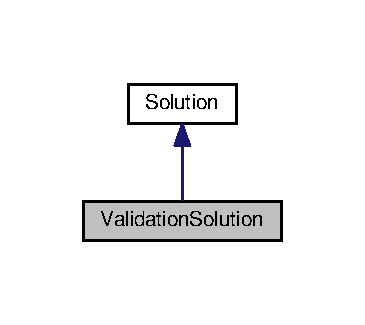
\includegraphics[width=175pt]{class_validation_solution__inherit__graph}
\end{center}
\end{figure}


Collaboration diagram for Validation\+Solution\+:\nopagebreak
\begin{figure}[H]
\begin{center}
\leavevmode
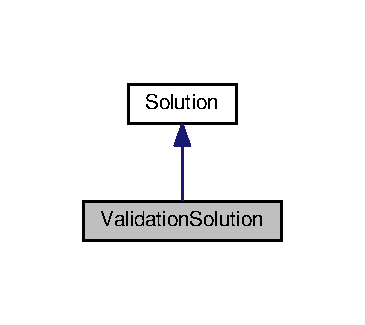
\includegraphics[width=175pt]{class_validation_solution__coll__graph}
\end{center}
\end{figure}


\subsection{Detailed Description}
\hyperlink{class_solution}{Solution} for the validation of a ML method. 

The documentation for this class was generated from the following file\+:\begin{DoxyCompactItemize}
\item 
includes/Validation\+Solution.\+hpp\end{DoxyCompactItemize}

\hypertarget{class_visualisation}{}\section{Visualisation Class Reference}
\label{class_visualisation}\index{Visualisation@{Visualisation}}


Class for visualize data using gnuplot.  




{\ttfamily \#include $<$Visualisation.\+hpp$>$}

\subsection*{Public Member Functions}
\begin{DoxyCompactItemize}
\item 
\mbox{\Hypertarget{class_visualisation_a7633f9b6b5350f8d6b6dd3e0aada0927}\label{class_visualisation_a7633f9b6b5350f8d6b6dd3e0aada0927}} 
{\bfseries Visualisation} (\hyperlink{class_data}{Data} $\ast$sample)
\item 
void \hyperlink{class_visualisation_a124977561c36f63108795e849ad0f100}{set\+Sample} (\hyperlink{class_data}{Data} sample)
\begin{DoxyCompactList}\small\item\em Set sample to be visualized. \end{DoxyCompactList}\item 
void \hyperlink{class_visualisation_ac217fcae4984edeb003bfcd208a253de}{set\+Title} (std\+::string title)
\begin{DoxyCompactList}\small\item\em Set plot title. \end{DoxyCompactList}\item 
void \hyperlink{class_visualisation_a2d29fee9180bcb2fd5cb6fc78253ac5b}{set\+Style} (std\+::string style)
\begin{DoxyCompactList}\small\item\em Set plot style. (points, lines, etc.) \end{DoxyCompactList}\item 
void \hyperlink{class_visualisation_a7569c77520391e6adf7e285410f4b358}{plot2D} (int x, int y)
\begin{DoxyCompactList}\small\item\em Plot the selected features in 2D. \end{DoxyCompactList}\item 
void \hyperlink{class_visualisation_a39cf83c146a4c92a32782bfdf6168594}{plot3D} (int x, int y, int z)
\begin{DoxyCompactList}\small\item\em Plot the selected features in 3D. \end{DoxyCompactList}\item 
void \hyperlink{class_visualisation_a39b7bd29878bfc2d21fc4219803fd99d}{plot2\+Dwith\+Hyperplane} (int x, int y, \hyperlink{class_solution}{Solution} w)
\begin{DoxyCompactList}\small\item\em Plot the data in 2D with separated by the hyperplane in the solution. \end{DoxyCompactList}\item 
void \hyperlink{class_visualisation_a3318af0b08322183e0dbe8d4891b580d}{plot3\+Dwith\+Hyperplane} (int x, int y, int z, \hyperlink{class_solution}{Solution} w)
\begin{DoxyCompactList}\small\item\em Plot the data in 2D with separated by the hyperplane in the solution. \end{DoxyCompactList}\end{DoxyCompactItemize}


\subsection{Detailed Description}
Class for visualize data using gnuplot. 

\subsection{Member Function Documentation}
\mbox{\Hypertarget{class_visualisation_a7569c77520391e6adf7e285410f4b358}\label{class_visualisation_a7569c77520391e6adf7e285410f4b358}} 
\index{Visualisation@{Visualisation}!plot2D@{plot2D}}
\index{plot2D@{plot2D}!Visualisation@{Visualisation}}
\subsubsection{\texorpdfstring{plot2\+D()}{plot2D()}}
{\footnotesize\ttfamily void Visualisation\+::plot2D (\begin{DoxyParamCaption}\item[{int}]{x,  }\item[{int}]{y }\end{DoxyParamCaption})}



Plot the selected features in 2D. 


\begin{DoxyParams}{Parameters}
{\em x} & (???) Feature to be used in the x-\/axis. \\
\hline
{\em y} & (???) Feature to be used in the y-\/axis. \\
\hline
\end{DoxyParams}
\begin{DoxyReturn}{Returns}
void 
\end{DoxyReturn}
\mbox{\Hypertarget{class_visualisation_a39b7bd29878bfc2d21fc4219803fd99d}\label{class_visualisation_a39b7bd29878bfc2d21fc4219803fd99d}} 
\index{Visualisation@{Visualisation}!plot2\+Dwith\+Hyperplane@{plot2\+Dwith\+Hyperplane}}
\index{plot2\+Dwith\+Hyperplane@{plot2\+Dwith\+Hyperplane}!Visualisation@{Visualisation}}
\subsubsection{\texorpdfstring{plot2\+Dwith\+Hyperplane()}{plot2DwithHyperplane()}}
{\footnotesize\ttfamily void Visualisation\+::plot2\+Dwith\+Hyperplane (\begin{DoxyParamCaption}\item[{int}]{x,  }\item[{int}]{y,  }\item[{\hyperlink{class_solution}{Solution}}]{w }\end{DoxyParamCaption})}



Plot the data in 2D with separated by the hyperplane in the solution. 


\begin{DoxyParams}{Parameters}
{\em x} & (???) Feature to be used in the x-\/axis. \\
\hline
{\em y} & (???) Feature to be used in the y-\/axis. \\
\hline
\end{DoxyParams}
\begin{DoxyReturn}{Returns}
void 
\end{DoxyReturn}
\mbox{\Hypertarget{class_visualisation_a39cf83c146a4c92a32782bfdf6168594}\label{class_visualisation_a39cf83c146a4c92a32782bfdf6168594}} 
\index{Visualisation@{Visualisation}!plot3D@{plot3D}}
\index{plot3D@{plot3D}!Visualisation@{Visualisation}}
\subsubsection{\texorpdfstring{plot3\+D()}{plot3D()}}
{\footnotesize\ttfamily void Visualisation\+::plot3D (\begin{DoxyParamCaption}\item[{int}]{x,  }\item[{int}]{y,  }\item[{int}]{z }\end{DoxyParamCaption})}



Plot the selected features in 3D. 


\begin{DoxyParams}{Parameters}
{\em x} & (???) Feature to be used in the x-\/axis. \\
\hline
{\em y} & (???) Feature to be used in the y-\/axis. \\
\hline
{\em z} & (???) Feature to be used in the z-\/axis. \\
\hline
\end{DoxyParams}
\begin{DoxyReturn}{Returns}
void 
\end{DoxyReturn}
\mbox{\Hypertarget{class_visualisation_a3318af0b08322183e0dbe8d4891b580d}\label{class_visualisation_a3318af0b08322183e0dbe8d4891b580d}} 
\index{Visualisation@{Visualisation}!plot3\+Dwith\+Hyperplane@{plot3\+Dwith\+Hyperplane}}
\index{plot3\+Dwith\+Hyperplane@{plot3\+Dwith\+Hyperplane}!Visualisation@{Visualisation}}
\subsubsection{\texorpdfstring{plot3\+Dwith\+Hyperplane()}{plot3DwithHyperplane()}}
{\footnotesize\ttfamily void Visualisation\+::plot3\+Dwith\+Hyperplane (\begin{DoxyParamCaption}\item[{int}]{x,  }\item[{int}]{y,  }\item[{int}]{z,  }\item[{\hyperlink{class_solution}{Solution}}]{w }\end{DoxyParamCaption})}



Plot the data in 2D with separated by the hyperplane in the solution. 


\begin{DoxyParams}{Parameters}
{\em x} & (???) Feature to be used in the x-\/axis. \\
\hline
{\em y} & (???) Feature to be used in the y-\/axis. \\
\hline
{\em z} & (???) Feature to be used in the z-\/axis. \\
\hline
\end{DoxyParams}
\begin{DoxyReturn}{Returns}
void 
\end{DoxyReturn}
\mbox{\Hypertarget{class_visualisation_a124977561c36f63108795e849ad0f100}\label{class_visualisation_a124977561c36f63108795e849ad0f100}} 
\index{Visualisation@{Visualisation}!set\+Sample@{set\+Sample}}
\index{set\+Sample@{set\+Sample}!Visualisation@{Visualisation}}
\subsubsection{\texorpdfstring{set\+Sample()}{setSample()}}
{\footnotesize\ttfamily void Visualisation\+::set\+Sample (\begin{DoxyParamCaption}\item[{\hyperlink{class_data}{Data}}]{sample }\end{DoxyParamCaption})}



Set sample to be visualized. 


\begin{DoxyParams}{Parameters}
{\em sample} & (???) \hyperlink{class_data}{Data} to set for visualization. \\
\hline
\end{DoxyParams}
\begin{DoxyReturn}{Returns}
void 
\end{DoxyReturn}
\mbox{\Hypertarget{class_visualisation_a2d29fee9180bcb2fd5cb6fc78253ac5b}\label{class_visualisation_a2d29fee9180bcb2fd5cb6fc78253ac5b}} 
\index{Visualisation@{Visualisation}!set\+Style@{set\+Style}}
\index{set\+Style@{set\+Style}!Visualisation@{Visualisation}}
\subsubsection{\texorpdfstring{set\+Style()}{setStyle()}}
{\footnotesize\ttfamily void Visualisation\+::set\+Style (\begin{DoxyParamCaption}\item[{std\+::string}]{style }\end{DoxyParamCaption})}



Set plot style. (points, lines, etc.) 


\begin{DoxyParams}{Parameters}
{\em style} & (???) Style to be set. \\
\hline
\end{DoxyParams}
\begin{DoxyReturn}{Returns}
void 
\end{DoxyReturn}
\mbox{\Hypertarget{class_visualisation_ac217fcae4984edeb003bfcd208a253de}\label{class_visualisation_ac217fcae4984edeb003bfcd208a253de}} 
\index{Visualisation@{Visualisation}!set\+Title@{set\+Title}}
\index{set\+Title@{set\+Title}!Visualisation@{Visualisation}}
\subsubsection{\texorpdfstring{set\+Title()}{setTitle()}}
{\footnotesize\ttfamily void Visualisation\+::set\+Title (\begin{DoxyParamCaption}\item[{std\+::string}]{title }\end{DoxyParamCaption})}



Set plot title. 


\begin{DoxyParams}{Parameters}
{\em title} & (???) Plot title. \\
\hline
\end{DoxyParams}
\begin{DoxyReturn}{Returns}
void 
\end{DoxyReturn}


The documentation for this class was generated from the following files\+:\begin{DoxyCompactItemize}
\item 
includes/Visualisation.\+hpp\item 
src/Visualisation.\+cpp\end{DoxyCompactItemize}

\chapter{File Documentation}
\hypertarget{_data_8hpp}{}\section{includes/\+Data.hpp File Reference}
\label{_data_8hpp}\index{includes/\+Data.\+hpp@{includes/\+Data.\+hpp}}
{\ttfamily \#include $<$vector$>$}\newline
{\ttfamily \#include $<$string$>$}\newline
{\ttfamily \#include $<$numeric$>$}\newline
{\ttfamily \#include $<$algorithm$>$}\newline
{\ttfamily \#include $<$sstream$>$}\newline
{\ttfamily \#include $<$iostream$>$}\newline
{\ttfamily \#include $<$fstream$>$}\newline
{\ttfamily \#include $<$memory$>$}\newline
{\ttfamily \#include \char`\"{}Point.\+hpp\char`\"{}}\newline
{\ttfamily \#include \char`\"{}Statistics.\+hpp\char`\"{}}\newline
{\ttfamily \#include \char`\"{}Utils.\+hpp\char`\"{}}\newline
Include dependency graph for Data.\+hpp\+:\nopagebreak
\begin{figure}[H]
\begin{center}
\leavevmode
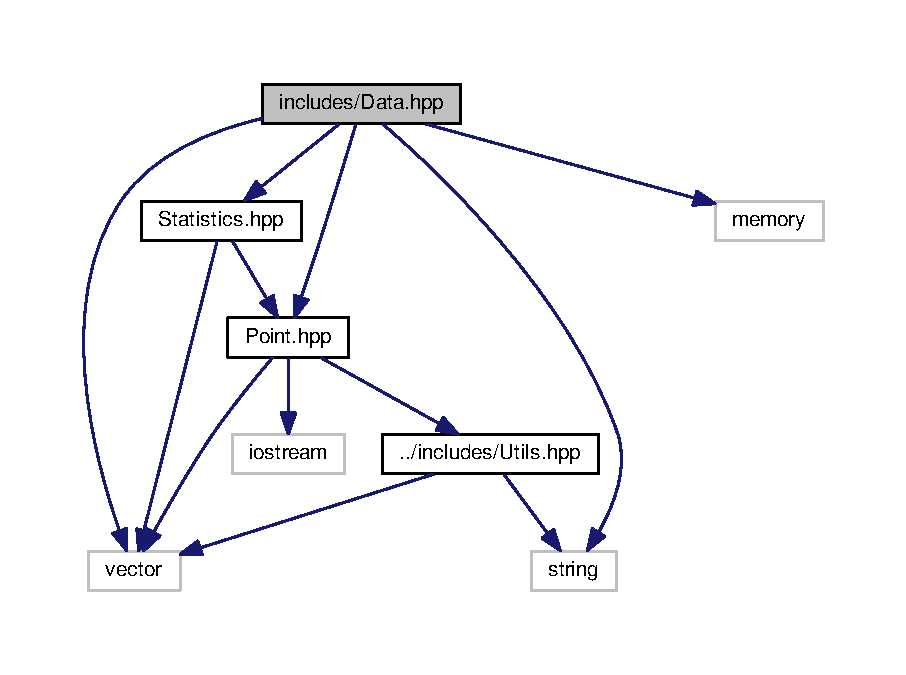
\includegraphics[width=350pt]{_data_8hpp__incl}
\end{center}
\end{figure}
This graph shows which files directly or indirectly include this file\+:\nopagebreak
\begin{figure}[H]
\begin{center}
\leavevmode
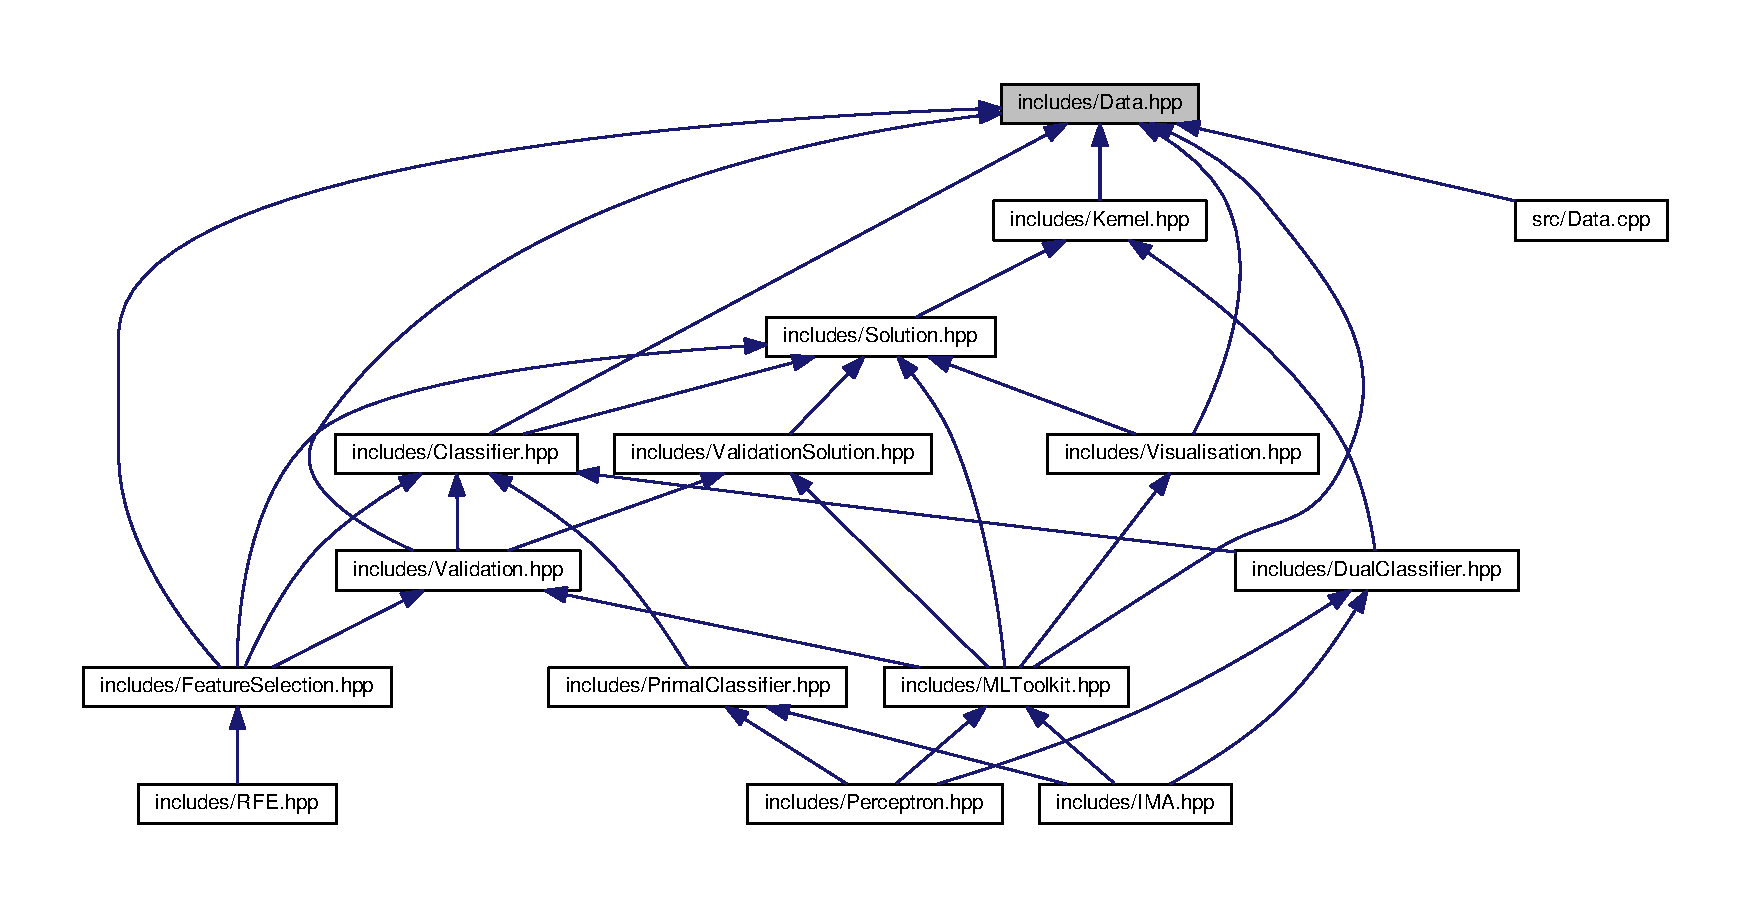
\includegraphics[width=350pt]{_data_8hpp__dep__incl}
\end{center}
\end{figure}
\subsection*{Data Structures}
\begin{DoxyCompactItemize}
\item 
class \hyperlink{class_data}{Data$<$ T $>$}
\begin{DoxyCompactList}\small\item\em Wrapper for the dataset data. \end{DoxyCompactList}\end{DoxyCompactItemize}
\subsection*{Enumerations}
\begin{DoxyCompactItemize}
\item 
\mbox{\Hypertarget{_data_8hpp_a1d1cfd8ffb84e947f82999c682b666a7}\label{_data_8hpp_a1d1cfd8ffb84e947f82999c682b666a7}} 
enum {\bfseries Type} \{ \newline
{\bfseries T\+Y\+P\+E\+\_\+\+I\+N\+V\+A\+L\+ID} = -\/1, 
{\bfseries T\+Y\+P\+E\+\_\+\+D\+A\+TA} = 0, 
{\bfseries T\+Y\+P\+E\+\_\+\+C\+SV} = 1, 
{\bfseries T\+Y\+P\+E\+\_\+\+A\+R\+FF} = 2, 
\newline
{\bfseries T\+Y\+P\+E\+\_\+\+T\+XT} = 3
 \}
\end{DoxyCompactItemize}
\subsection*{Functions}
\begin{DoxyCompactItemize}
\item 
\mbox{\Hypertarget{_data_8hpp_a4e6c3141b57fb6582acc4dac8f62a891}\label{_data_8hpp_a4e6c3141b57fb6582acc4dac8f62a891}} 
{\footnotesize template$<$typename T $>$ }\\ostream \& {\bfseries operator$<$$<$} (ostream \&output, const \hyperlink{class_data}{Data}$<$ T $>$ \&data)
\end{DoxyCompactItemize}


\subsection{Detailed Description}
\hyperlink{class_data}{Data} manipulation class

\begin{DoxyAuthor}{Author}
Mateus Coutinho Marim 
\end{DoxyAuthor}

\hypertarget{_perceptron_8hpp}{}\section{includes/\+Perceptron.hpp File Reference}
\label{_perceptron_8hpp}\index{includes/\+Perceptron.\+hpp@{includes/\+Perceptron.\+hpp}}
{\ttfamily \#include \char`\"{}Primal\+Classifier.\+hpp\char`\"{}}\newline
{\ttfamily \#include \char`\"{}Dual\+Classifier.\+hpp\char`\"{}}\newline
{\ttfamily \#include \char`\"{}M\+L\+Toolkit.\+hpp\char`\"{}}\newline
Include dependency graph for Perceptron.\+hpp\+:
% FIG 0
\subsection*{Data Structures}
\begin{DoxyCompactItemize}
\item 
class \mbox{\hyperlink{class_perceptron_primal}{Perceptron\+Primal$<$ T $>$}}
\begin{DoxyCompactList}\small\item\em Wrapper for the implementation of the Perceptron primal algorithm. \end{DoxyCompactList}\item 
class \mbox{\hyperlink{class_perceptron_fixed_margin_primal}{Perceptron\+Fixed\+Margin\+Primal$<$ T $>$}}
\begin{DoxyCompactList}\small\item\em Wrapper for the implementation of the Perceptron primal with fixed margin algorithm. \end{DoxyCompactList}\item 
class \mbox{\hyperlink{class_perceptron_dual}{Perceptron\+Dual$<$ T $>$}}
\begin{DoxyCompactList}\small\item\em Wrapper for the implementation of the Perceptron dual algorithm. \end{DoxyCompactList}\item 
class \mbox{\hyperlink{class_perceptron_fixed_margin_dual}{Perceptron\+Fixed\+Margin\+Dual$<$ T $>$}}
\begin{DoxyCompactList}\small\item\em Wrapper for the implementation of the Perceptron dual with fixed margin algorithm. \end{DoxyCompactList}\end{DoxyCompactItemize}


\subsection{Detailed Description}
Perceptron algorithm implementations

\begin{DoxyAuthor}{Author}
Mateus Coutinho Marim 
\end{DoxyAuthor}

\hypertarget{_random_8hpp}{}\section{includes/\+Random.hpp File Reference}
\label{_random_8hpp}\index{includes/\+Random.\+hpp@{includes/\+Random.\+hpp}}
{\ttfamily \#include $<$random$>$}\newline
{\ttfamily \#include $<$functional$>$}\newline
Include dependency graph for Random.\+hpp\+:\nopagebreak
\begin{figure}[H]
\begin{center}
\leavevmode
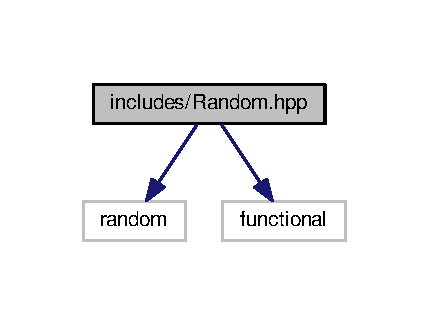
\includegraphics[width=206pt]{_random_8hpp__incl}
\end{center}
\end{figure}
\subsection*{Functions}
\begin{DoxyCompactItemize}
\item 
\mbox{\Hypertarget{_random_8hpp_ad8b845768c2e5f049eb7ae06955bdd77}\label{_random_8hpp_ad8b845768c2e5f049eb7ae06955bdd77}} 
auto {\bfseries Random\+::init} (unsigned int seed=666)
\item 
\mbox{\Hypertarget{_random_8hpp_a0fecb2ca9c3ca82f87c35ceed7146ffe}\label{_random_8hpp_a0fecb2ca9c3ca82f87c35ceed7146ffe}} 
int {\bfseries Random\+::int\+In\+Range} (int low, int high)
\item 
\mbox{\Hypertarget{_random_8hpp_ac99d2b48fd9c53d096da24b17227c0a3}\label{_random_8hpp_ac99d2b48fd9c53d096da24b17227c0a3}} 
float {\bfseries Random\+::float\+In\+Range} (float low, float high)
\item 
\mbox{\Hypertarget{_random_8hpp_a928dacbcc057819706ba38bc20046035}\label{_random_8hpp_a928dacbcc057819706ba38bc20046035}} 
auto {\bfseries Random\+::get\+Seed} ()
\end{DoxyCompactItemize}
\subsection*{Variables}
\begin{DoxyCompactItemize}
\item 
\mbox{\Hypertarget{_random_8hpp_aacd664e02f96dd6df8a91ad18d47139e}\label{_random_8hpp_aacd664e02f96dd6df8a91ad18d47139e}} 
std\+::mt19937 {\bfseries Random\+::m\+\_\+gen}
\item 
\mbox{\Hypertarget{_random_8hpp_afb7dc062df38f99a2e878bfef6109d4c}\label{_random_8hpp_afb7dc062df38f99a2e878bfef6109d4c}} 
unsigned int {\bfseries Random\+::m\+\_\+seed}
\end{DoxyCompactItemize}


\subsection{Detailed Description}
Random namespace

\begin{DoxyAuthor}{Author}
Mateus Coutinho Marim 
\end{DoxyAuthor}

\hypertarget{_timer_8hpp}{}\section{includes/\+Timer.hpp File Reference}
\label{_timer_8hpp}\index{includes/\+Timer.\+hpp@{includes/\+Timer.\+hpp}}
{\ttfamily \#include $<$chrono$>$}\newline
Include dependency graph for Timer.\+hpp\+:\nopagebreak
\begin{figure}[H]
\begin{center}
\leavevmode
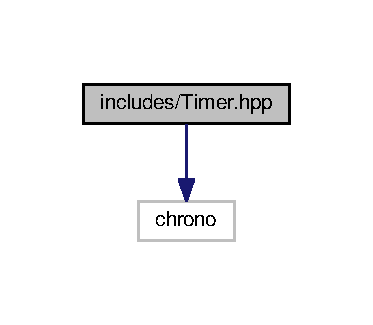
\includegraphics[width=179pt]{_timer_8hpp__incl}
\end{center}
\end{figure}
This graph shows which files directly or indirectly include this file\+:\nopagebreak
\begin{figure}[H]
\begin{center}
\leavevmode
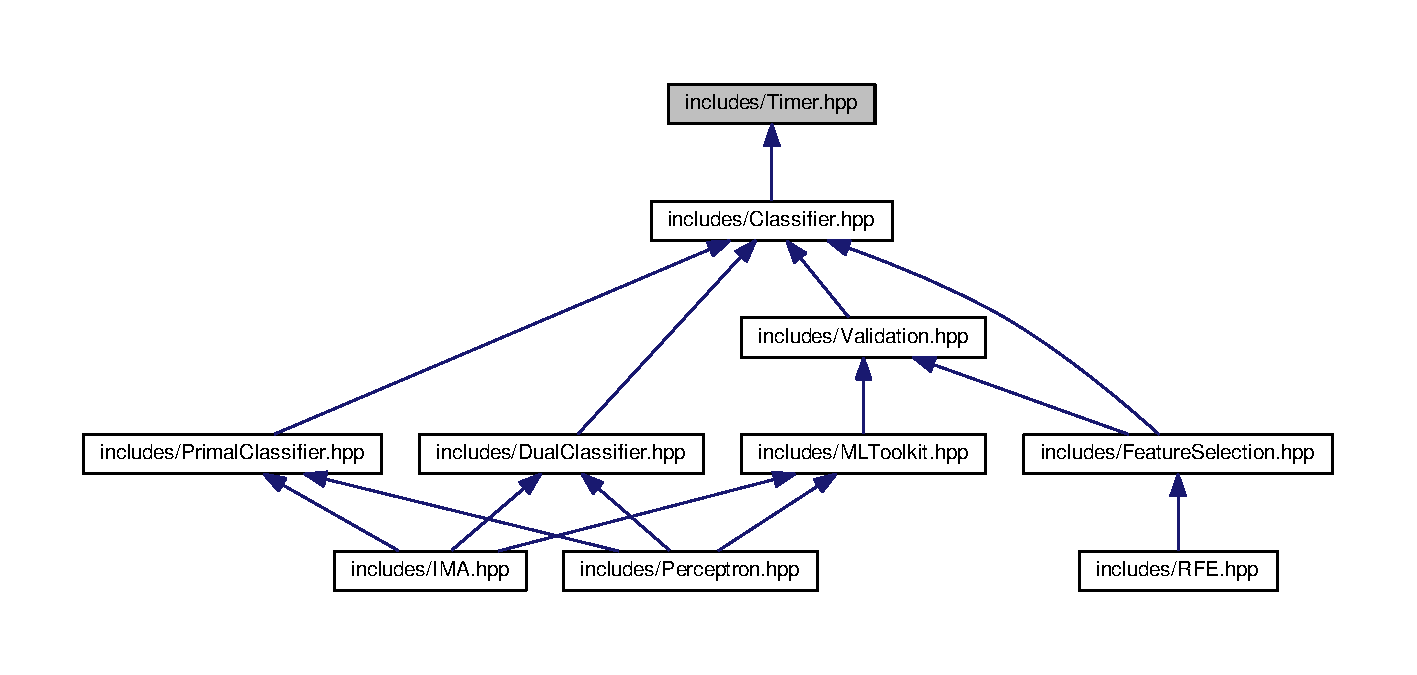
\includegraphics[width=350pt]{_timer_8hpp__dep__incl}
\end{center}
\end{figure}
\subsection*{Data Structures}
\begin{DoxyCompactItemize}
\item 
class \hyperlink{class_timer}{Timer}
\end{DoxyCompactItemize}


\subsection{Detailed Description}
\hyperlink{class_timer}{Timer} class

\begin{DoxyAuthor}{Author}
Mateus Coutinho Marim 
\end{DoxyAuthor}

\hypertarget{_utils_8hpp}{}\section{includes/\+Utils.hpp File Reference}
\label{_utils_8hpp}\index{includes/\+Utils.\+hpp@{includes/\+Utils.\+hpp}}
{\ttfamily \#include $<$string$>$}\newline
{\ttfamily \#include $<$vector$>$}\newline
Include dependency graph for Utils.\+hpp\+:\nopagebreak
\begin{figure}[H]
\begin{center}
\leavevmode
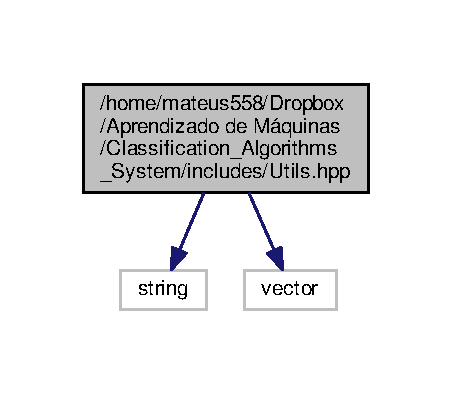
\includegraphics[width=184pt]{_utils_8hpp__incl}
\end{center}
\end{figure}
This graph shows which files directly or indirectly include this file\+:
\nopagebreak
\begin{figure}[H]
\begin{center}
\leavevmode
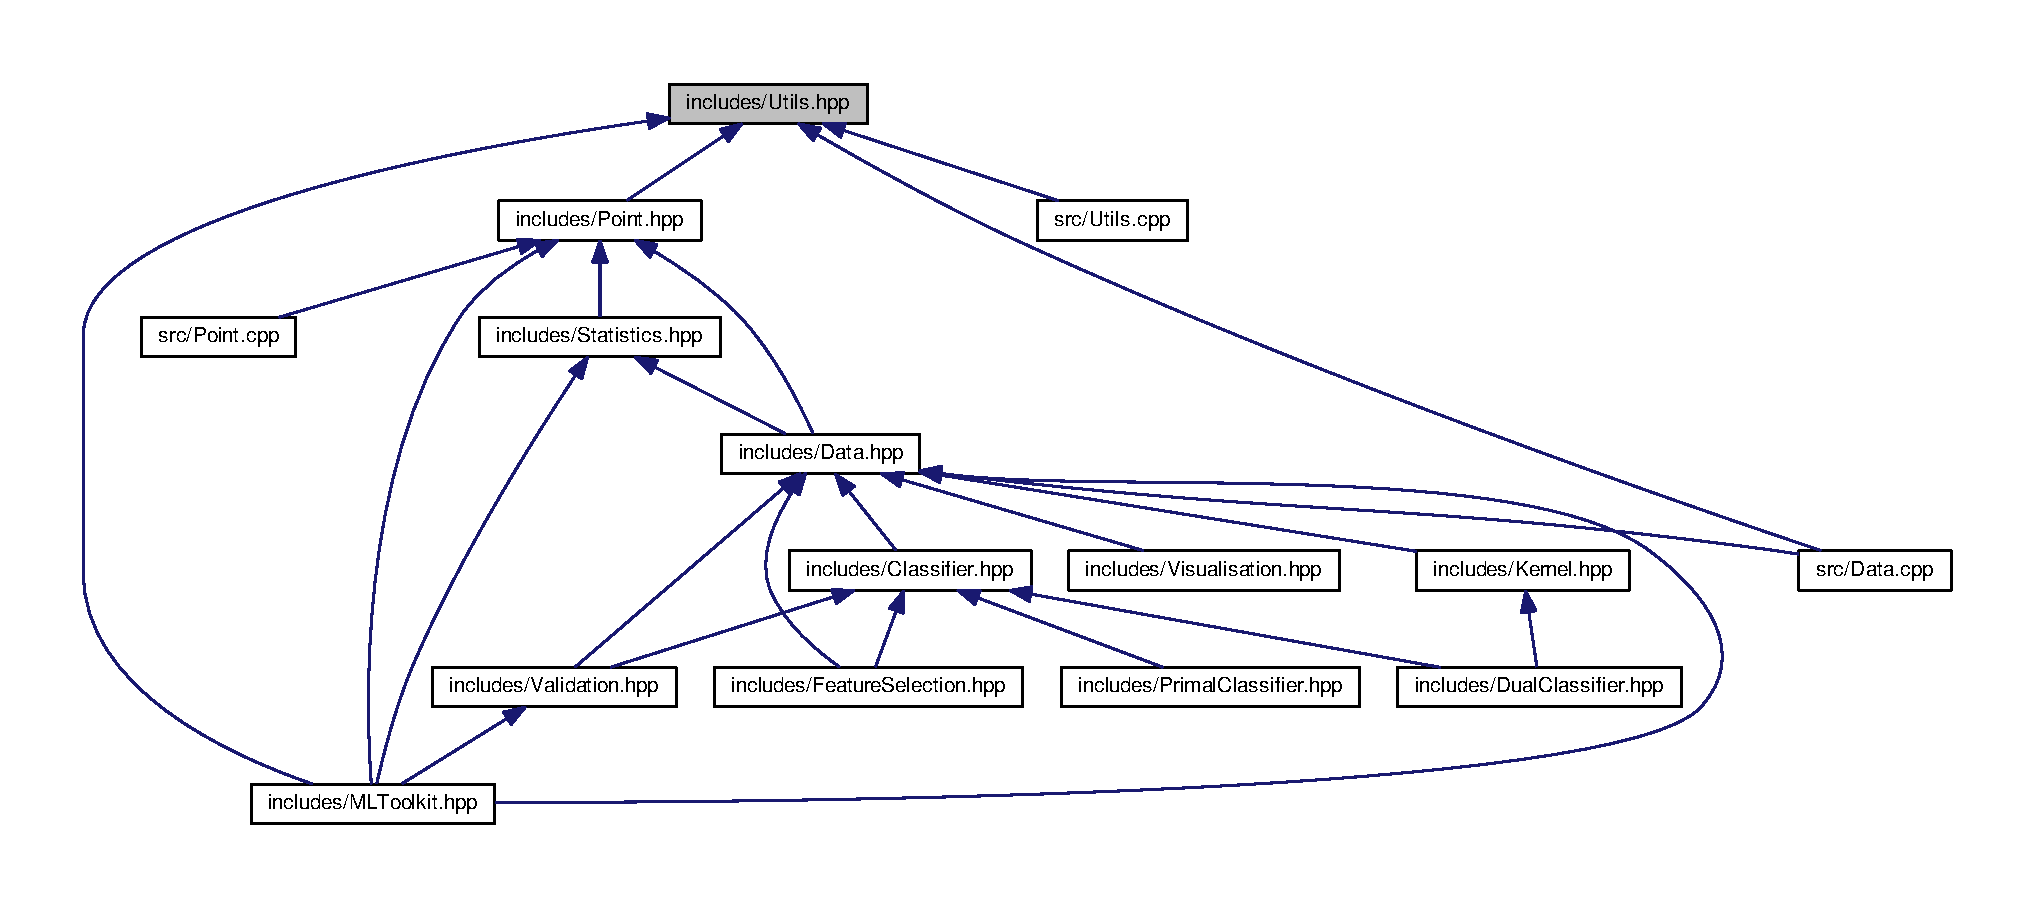
\includegraphics[width=350pt]{_utils_8hpp__dep__incl}
\end{center}
\end{figure}
\subsection*{Macros}
\begin{DoxyCompactItemize}
\item 
\mbox{\Hypertarget{_utils_8hpp_a12c2040f25d8e3a7b9e1c2024c618cb6}\label{_utils_8hpp_a12c2040f25d8e3a7b9e1c2024c618cb6}} 
\#define {\bfseries I\+NF}~1\+E8
\end{DoxyCompactItemize}
\subsection*{Typedefs}
\begin{DoxyCompactItemize}
\item 
\mbox{\Hypertarget{_utils_8hpp_a5b939e9afe8dd07c1182ecede20c61b1}\label{_utils_8hpp_a5b939e9afe8dd07c1182ecede20c61b1}} 
typedef std\+::vector$<$ std\+::vector$<$ double $>$ $>$ {\bfseries d\+Matrix}
\end{DoxyCompactItemize}
\subsection*{Enumerations}
\begin{DoxyCompactItemize}
\item 
\mbox{\Hypertarget{_utils_8hpp_ad4bb8dabdbf8ad75e34220cc666b59ca}\label{_utils_8hpp_ad4bb8dabdbf8ad75e34220cc666b59ca}} 
enum {\bfseries Norm\+Type} \{ {\bfseries N\+O\+R\+M\+\_\+\+L\+I\+NF} = 0, 
{\bfseries N\+O\+R\+M\+\_\+\+L1} = 1, 
{\bfseries N\+O\+R\+M\+\_\+\+L2} = 2
 \}
\end{DoxyCompactItemize}
\subsection*{Functions}
\begin{DoxyCompactItemize}
\item 
bool \hyperlink{_utils_8hpp_ad5057d992c7e88f80c37a28044320e45}{is\+\_\+number} (std\+::string str)
\begin{DoxyCompactList}\small\item\em Verify if the string is a number. \end{DoxyCompactList}\item 
int \hyperlink{_utils_8hpp_a8f8f36f1e1b6c6900fac56c148f754eb}{stoin} (std\+::string str)
\begin{DoxyCompactList}\small\item\em Converts the string to an integer. \end{DoxyCompactList}\item 
double \hyperlink{_utils_8hpp_a0187e008853de2faa4269af7602af7d5}{stodn} (std\+::string str)
\begin{DoxyCompactList}\small\item\em Converts the string to a double. \end{DoxyCompactList}\item 
double \hyperlink{_utils_8hpp_a79ab62c544d771819865bec0eb8e5360}{max\+Abs\+Element} (std\+::vector$<$ double $>$ x)
\begin{DoxyCompactList}\small\item\em Returns the max absolute element. \end{DoxyCompactList}\end{DoxyCompactItemize}


\subsection{Detailed Description}
Utils functions

\begin{DoxyAuthor}{Author}
Mateus Coutinho Marim 
\end{DoxyAuthor}


\subsection{Function Documentation}
\mbox{\Hypertarget{_utils_8hpp_ad5057d992c7e88f80c37a28044320e45}\label{_utils_8hpp_ad5057d992c7e88f80c37a28044320e45}} 
\index{Utils.\+hpp@{Utils.\+hpp}!is\+\_\+number@{is\+\_\+number}}
\index{is\+\_\+number@{is\+\_\+number}!Utils.\+hpp@{Utils.\+hpp}}
\subsubsection{\texorpdfstring{is\+\_\+number()}{is\_number()}}
{\footnotesize\ttfamily bool is\+\_\+number (\begin{DoxyParamCaption}\item[{std\+::string}]{str }\end{DoxyParamCaption})}



Verify if the string is a number. 


\begin{DoxyParams}{Parameters}
{\em str} & String to be tested. \\
\hline
\end{DoxyParams}
\begin{DoxyReturn}{Returns}
bool 
\end{DoxyReturn}
\mbox{\Hypertarget{_utils_8hpp_a79ab62c544d771819865bec0eb8e5360}\label{_utils_8hpp_a79ab62c544d771819865bec0eb8e5360}} 
\index{Utils.\+hpp@{Utils.\+hpp}!max\+Abs\+Element@{max\+Abs\+Element}}
\index{max\+Abs\+Element@{max\+Abs\+Element}!Utils.\+hpp@{Utils.\+hpp}}
\subsubsection{\texorpdfstring{max\+Abs\+Element()}{maxAbsElement()}}
{\footnotesize\ttfamily double max\+Abs\+Element (\begin{DoxyParamCaption}\item[{std\+::vector$<$ double $>$}]{x }\end{DoxyParamCaption})}



Returns the max absolute element. 


\begin{DoxyParams}{Parameters}
{\em x} & The vector used to obtain the max element. \\
\hline
\end{DoxyParams}
\begin{DoxyReturn}{Returns}
The max absolute element found. 
\end{DoxyReturn}
\mbox{\Hypertarget{_utils_8hpp_a0187e008853de2faa4269af7602af7d5}\label{_utils_8hpp_a0187e008853de2faa4269af7602af7d5}} 
\index{Utils.\+hpp@{Utils.\+hpp}!stodn@{stodn}}
\index{stodn@{stodn}!Utils.\+hpp@{Utils.\+hpp}}
\subsubsection{\texorpdfstring{stodn()}{stodn()}}
{\footnotesize\ttfamily double stodn (\begin{DoxyParamCaption}\item[{std\+::string}]{str }\end{DoxyParamCaption})}



Converts the string to a double. 


\begin{DoxyParams}{Parameters}
{\em str} & The string to be converted. \\
\hline
\end{DoxyParams}
\begin{DoxyReturn}{Returns}
The double resulted from the conversion. 
\end{DoxyReturn}
\mbox{\Hypertarget{_utils_8hpp_a8f8f36f1e1b6c6900fac56c148f754eb}\label{_utils_8hpp_a8f8f36f1e1b6c6900fac56c148f754eb}} 
\index{Utils.\+hpp@{Utils.\+hpp}!stoin@{stoin}}
\index{stoin@{stoin}!Utils.\+hpp@{Utils.\+hpp}}
\subsubsection{\texorpdfstring{stoin()}{stoin()}}
{\footnotesize\ttfamily int stoin (\begin{DoxyParamCaption}\item[{std\+::string}]{str }\end{DoxyParamCaption})}



Converts the string to an integer. 


\begin{DoxyParams}{Parameters}
{\em str} & String to be converted. \\
\hline
\end{DoxyParams}
\begin{DoxyReturn}{Returns}
The integer resulted from the conversion. 
\end{DoxyReturn}

\hypertarget{_data_8cpp}{}\section{/home/mateus558/\+Dropbox/\+Aprendizado de Máquinas/\+Classification\+\_\+\+Algorithms\+\_\+\+System/src/\+Data.cpp File Reference}
\label{_data_8cpp}\index{/home/mateus558/\+Dropbox/\+Aprendizado de Máquinas/\+Classification\+\_\+\+Algorithms\+\_\+\+System/src/\+Data.\+cpp@{/home/mateus558/\+Dropbox/\+Aprendizado de Máquinas/\+Classification\+\_\+\+Algorithms\+\_\+\+System/src/\+Data.\+cpp}}


Implementation of the \hyperlink{class_data}{Data} class methods.  


{\ttfamily \#include $<$iostream$>$}\newline
{\ttfamily \#include $<$vector$>$}\newline
{\ttfamily \#include $<$algorithm$>$}\newline
{\ttfamily \#include $<$numeric$>$}\newline
{\ttfamily \#include $<$sstream$>$}\newline
{\ttfamily \#include $<$iterator$>$}\newline
{\ttfamily \#include $<$fstream$>$}\newline
{\ttfamily \#include $<$ctime$>$}\newline
{\ttfamily \#include $<$cmath$>$}\newline
{\ttfamily \#include $<$cstdio$>$}\newline
{\ttfamily \#include \char`\"{}../includes/\+Data.\+hpp\char`\"{}}\newline
{\ttfamily \#include \char`\"{}../includes/\+Utils.\+hpp\char`\"{}}\newline
Include dependency graph for Data.\+cpp\+:\nopagebreak
\begin{figure}[H]
\begin{center}
\leavevmode
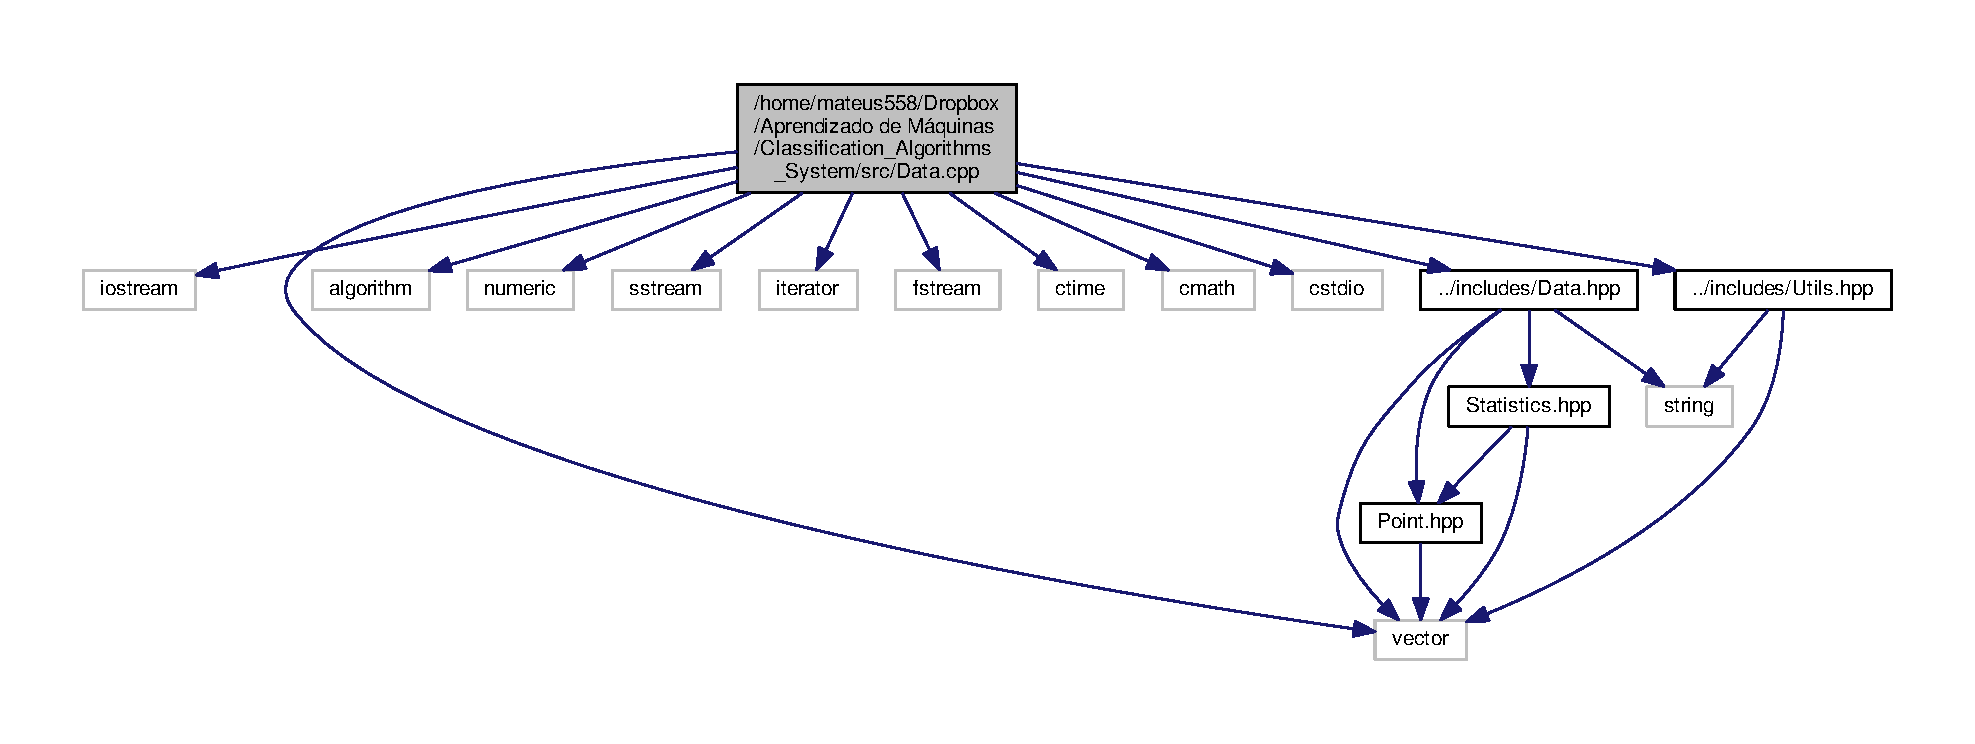
\includegraphics[width=350pt]{_data_8cpp__incl}
\end{center}
\end{figure}


\subsection{Detailed Description}
Implementation of the \hyperlink{class_data}{Data} class methods. 


\hypertarget{_point_8cpp}{}\section{src/\+Point.cpp File Reference}
\label{_point_8cpp}\index{src/\+Point.\+cpp@{src/\+Point.\+cpp}}


Implementation of the \hyperlink{class_point}{Point} class methods.  


{\ttfamily \#include $<$iostream$>$}\newline
{\ttfamily \#include $<$cmath$>$}\newline
{\ttfamily \#include \char`\"{}../includes/\+Point.\+hpp\char`\"{}}\newline
{\ttfamily \#include \char`\"{}../includes/\+Utils.\+hpp\char`\"{}}\newline
Include dependency graph for Point.\+cpp\+:
\nopagebreak
\begin{figure}[H]
\begin{center}
\leavevmode
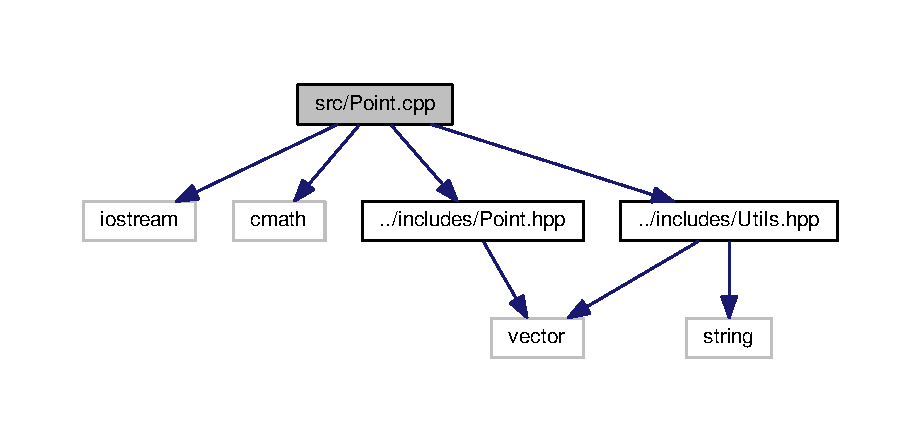
\includegraphics[width=350pt]{_point_8cpp__incl}
\end{center}
\end{figure}


\subsection{Detailed Description}
Implementation of the \hyperlink{class_point}{Point} class methods. 


\hypertarget{_utils_8cpp}{}\section{src/\+Utils.cpp File Reference}
\label{_utils_8cpp}\index{src/\+Utils.\+cpp@{src/\+Utils.\+cpp}}


Implementation of methods for general use in the system.  


{\ttfamily \#include $<$cmath$>$}\\*
{\ttfamily \#include $<$cstring$>$}\\*
{\ttfamily \#include $<$sstream$>$}\\*
{\ttfamily \#include \char`\"{}../includes/\+Utils.\+hpp\char`\"{}}\\*
Include dependency graph for Utils.\+cpp\+:
\nopagebreak
\begin{figure}[H]
\begin{center}
\leavevmode
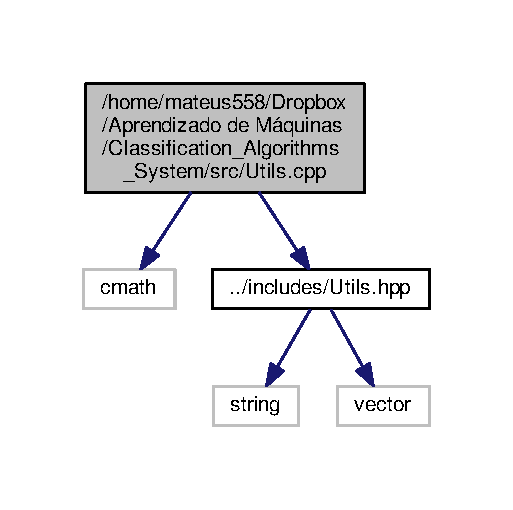
\includegraphics[width=350pt]{_utils_8cpp__incl}
\end{center}
\end{figure}
\subsection*{Macros}
\begin{DoxyCompactItemize}
\item 
\#define {\bfseries P\+R\+E\+C\+I\+S\+I\+ON}~1\+E-\/9\hypertarget{_utils_8cpp_a9c7b069fee3c8184e14a7de8e5da2dc6}{}\label{_utils_8cpp_a9c7b069fee3c8184e14a7de8e5da2dc6}

\item 
\#define {\bfseries M\+A\+X\+\_\+\+N\+U\+M\+B\+E\+R\+\_\+\+S\+T\+R\+I\+N\+G\+\_\+\+S\+I\+ZE}~32\hypertarget{_utils_8cpp_a7873e5175e32a7777d5f4761791b0126}{}\label{_utils_8cpp_a7873e5175e32a7777d5f4761791b0126}

\end{DoxyCompactItemize}
\subsection*{Functions}
\begin{DoxyCompactItemize}
\item 
bool \hyperlink{_utils_8cpp_a023a5c6fa42981cbd7b582ee1b214e7b}{is\+\_\+number} (string str)
\begin{DoxyCompactList}\small\item\em Verify if the string is a number. \end{DoxyCompactList}\item 
int \hyperlink{_utils_8cpp_a32f98cacc8ec2ab7033423e3a85572da}{stoin} (string str)
\begin{DoxyCompactList}\small\item\em Converts the string to an integer. \end{DoxyCompactList}\item 
double {\bfseries atof} (char s\mbox{[}$\,$\mbox{]})\hypertarget{_utils_8cpp_a0255102cc0c35b55cddf49a42e760695}{}\label{_utils_8cpp_a0255102cc0c35b55cddf49a42e760695}

\item 
double \hyperlink{_utils_8cpp_a5a71f54c5a674098cd327eb73ef77149}{stodn} (string str)
\begin{DoxyCompactList}\small\item\em Converts the string to a double. \end{DoxyCompactList}\item 
string \hyperlink{_utils_8cpp_a26f5a4cacb0634afa02adbeebd3f023c}{itos} (int n)
\begin{DoxyCompactList}\small\item\em itos Integer to string conversion. \end{DoxyCompactList}\item 
void {\bfseries reverse} (char $\ast$str, int len)\hypertarget{_utils_8cpp_aad7fea725cb4b198ace1aa3df5051244}{}\label{_utils_8cpp_aad7fea725cb4b198ace1aa3df5051244}

\item 
int {\bfseries int\+To\+Str} (int x, char str\mbox{[}$\,$\mbox{]}, int d)\hypertarget{_utils_8cpp_a631933fa325410873e33addc6c4bb24a}{}\label{_utils_8cpp_a631933fa325410873e33addc6c4bb24a}

\item 
string \hyperlink{_utils_8cpp_a275d36ee09955d83c3c2433d10088a04}{dtoa} (double n)
\begin{DoxyCompactList}\small\item\em dtoa Double to string conversion. \end{DoxyCompactList}\item 
{\footnotesize template$<$typename Out $>$ }\\void {\bfseries split} (const std\+::string \&s, char delim, Out result)\hypertarget{_utils_8cpp_a03529396588a5d4dac36c432989fdfaa}{}\label{_utils_8cpp_a03529396588a5d4dac36c432989fdfaa}

\item 
std\+::vector$<$ std\+::string $>$ {\bfseries split} (const std\+::string \&s, char delim)\hypertarget{_utils_8cpp_ae924c9b43cd7b086945003c09c294d2b}{}\label{_utils_8cpp_ae924c9b43cd7b086945003c09c294d2b}

\end{DoxyCompactItemize}


\subsection{Detailed Description}
Implementation of methods for general use in the system. 

Utils functions \begin{DoxyAuthor}{Author}
Mateus Coutinho Marim 
\end{DoxyAuthor}


\subsection{Function Documentation}
\index{Utils.\+cpp@{Utils.\+cpp}!dtoa@{dtoa}}
\index{dtoa@{dtoa}!Utils.\+cpp@{Utils.\+cpp}}
\subsubsection[{\texorpdfstring{dtoa(double n)}{dtoa(double n)}}]{\setlength{\rightskip}{0pt plus 5cm}string dtoa (
\begin{DoxyParamCaption}
\item[{double}]{n}
\end{DoxyParamCaption}
)}\hypertarget{_utils_8cpp_a275d36ee09955d83c3c2433d10088a04}{}\label{_utils_8cpp_a275d36ee09955d83c3c2433d10088a04}


dtoa Double to string conversion. 


\begin{DoxyParams}{Parameters}
{\em n} & Double to be converted. \\
\hline
\end{DoxyParams}
\begin{DoxyReturn}{Returns}
string 
\end{DoxyReturn}
\index{Utils.\+cpp@{Utils.\+cpp}!is\+\_\+number@{is\+\_\+number}}
\index{is\+\_\+number@{is\+\_\+number}!Utils.\+cpp@{Utils.\+cpp}}
\subsubsection[{\texorpdfstring{is\+\_\+number(string str)}{is_number(string str)}}]{\setlength{\rightskip}{0pt plus 5cm}bool is\+\_\+number (
\begin{DoxyParamCaption}
\item[{std\+::string}]{str}
\end{DoxyParamCaption}
)}\hypertarget{_utils_8cpp_a023a5c6fa42981cbd7b582ee1b214e7b}{}\label{_utils_8cpp_a023a5c6fa42981cbd7b582ee1b214e7b}


Verify if the string is a number. 


\begin{DoxyParams}{Parameters}
{\em str} & String to be tested. \\
\hline
\end{DoxyParams}
\begin{DoxyReturn}{Returns}
bool 
\end{DoxyReturn}
\index{Utils.\+cpp@{Utils.\+cpp}!itos@{itos}}
\index{itos@{itos}!Utils.\+cpp@{Utils.\+cpp}}
\subsubsection[{\texorpdfstring{itos(int n)}{itos(int n)}}]{\setlength{\rightskip}{0pt plus 5cm}string itos (
\begin{DoxyParamCaption}
\item[{int}]{n}
\end{DoxyParamCaption}
)}\hypertarget{_utils_8cpp_a26f5a4cacb0634afa02adbeebd3f023c}{}\label{_utils_8cpp_a26f5a4cacb0634afa02adbeebd3f023c}


itos Integer to string conversion. 


\begin{DoxyParams}{Parameters}
{\em n} & Integer to be converted. \\
\hline
\end{DoxyParams}
\begin{DoxyReturn}{Returns}
string 
\end{DoxyReturn}
\index{Utils.\+cpp@{Utils.\+cpp}!stodn@{stodn}}
\index{stodn@{stodn}!Utils.\+cpp@{Utils.\+cpp}}
\subsubsection[{\texorpdfstring{stodn(string str)}{stodn(string str)}}]{\setlength{\rightskip}{0pt plus 5cm}double stodn (
\begin{DoxyParamCaption}
\item[{std\+::string}]{str}
\end{DoxyParamCaption}
)}\hypertarget{_utils_8cpp_a5a71f54c5a674098cd327eb73ef77149}{}\label{_utils_8cpp_a5a71f54c5a674098cd327eb73ef77149}


Converts the string to a double. 


\begin{DoxyParams}{Parameters}
{\em str} & The string to be converted. \\
\hline
\end{DoxyParams}
\begin{DoxyReturn}{Returns}
The double resulted from the conversion. 
\end{DoxyReturn}
\index{Utils.\+cpp@{Utils.\+cpp}!stoin@{stoin}}
\index{stoin@{stoin}!Utils.\+cpp@{Utils.\+cpp}}
\subsubsection[{\texorpdfstring{stoin(string str)}{stoin(string str)}}]{\setlength{\rightskip}{0pt plus 5cm}int stoin (
\begin{DoxyParamCaption}
\item[{std\+::string}]{str}
\end{DoxyParamCaption}
)}\hypertarget{_utils_8cpp_a32f98cacc8ec2ab7033423e3a85572da}{}\label{_utils_8cpp_a32f98cacc8ec2ab7033423e3a85572da}


Converts the string to an integer. 


\begin{DoxyParams}{Parameters}
{\em str} & String to be converted. \\
\hline
\end{DoxyParams}
\begin{DoxyReturn}{Returns}
The integer resulted from the conversion. 
\end{DoxyReturn}

%--- End generated contents ---

% Index
\backmatter
\newpage
\phantomsection
\clearemptydoublepage
\addcontentsline{toc}{chapter}{Index}
\printindex

\end{document}
